%%%%%%%%%%%%%%%%%%%%%%%%%%%%%%%%%%%%%%%%%%%%%%%%%%%%%%%%%%%%%%%%%%% 
%                                                                 %
%                            ROOT FILE                            %
%                                                                 %
%%%%%%%%%%%%%%%%%%%%%%%%%%%%%%%%%%%%%%%%%%%%%%%%%%%%%%%%%%%%%%%%%%% 
%
%  Run LaTeX or pdfLaTeX on this file to produce your thesis.
%  To produce the abstract title page followed by the abstract,
%  see the file abstitle-phd.tex or abstitle-mas.tex.
%
%%%%%%%%%%%j %%%%%%%%%%%%%%%%%%%%%%%%%%%%%%%%%%%%%%%%%%%%%%%%%%%%%%%%

\documentclass[chap]{thesis}

% ------------------------
% You MUST attribute any previously published work (even if it's your own writing)
% Attribution of previously published work
% Use the after title and before the first sentence of the chapter.
% Example: \blfootnote{This work perviously appeared as: \bibentry{mypaper2015}
\makeatletter
\def\blfootnote{\xdef\@thefnmark{}\@footnotetext}
\makeatother
\usepackage{bibentry}
\nobibliography*

% If you have an attribution before your first in-text citation, 
% you should use \nobibentry to ensure in-text citations start at [1]
\newcommand{\ignore}[1]{}
\newcommand{\nobibentry}[1]{{\let\nocite\ignore\bibentry{#1}}}
% ------------------------


% insert watermark on first page to indicate this document is the dissertation proposal.
%\usepackage[firstpage]{draftwatermark}
\usepackage[colorlinks,citecolor=black,linkcolor=black]{hyperref}
\usepackage{amsmath}
\usepackage{rotating}
\usepackage[autostyle]{csquotes}
\usepackage{enumitem}
%\usepackage{adjustbox}


\newcommand{\lmodality}[1]{%
  \ensuremath{\mathbf{#1}}}
\newcommand{\defmodality}[2]{%
  \newcommand{#1}{\lmodality{#2}}}
\defmodality{\common}{C}
\defmodality{\knows}{K}
\defmodality{\believes}{B}
\defmodality{\perceives}{P}
\defmodality{\desires}{D}
\defmodality{\intends}{I}
\defmodality{\says}{S}

\newcommand{\lsymbol}[1]{%
  \ensuremath{\mathit{#1}}}
\newcommand{\defsymbol}[2]{%
  \newcommand{#1}{\lsymbol{#2}}}
\defsymbol{\action}{action}
\defsymbol{\initially}{initially}
\defsymbol{\holds}{holds}
\defsymbol{\happens}{happens}
\defsymbol{\clipped}{clipped}
\defsymbol{\initiates}{initiates}
\defsymbol{\terminates}{terminates}
\defsymbol{\prior}{prior}
\defsymbol{\interval}{interval}

\defsymbol{\guilty}{guilty}
\defsymbol{\Doctorshopping}{Doctorshopping}
\defsymbol{\getrx}{getrx}
\defsymbol{\tells}{tells}
\defsymbol{\duration}{duration}
\defsymbol{\tone}{t1}
\defsymbol{\ttwo}{t2}
\defsymbol{\tthree}{t3}
\defsymbol{\done}{d1}
\defsymbol{\dtwo}{d2}
\defsymbol{\dthree}{d3}
\defsymbol{\Blue}{Blue}
\defsymbol{\Lexapro}{Lexapro}
\defsymbol{\DrWhite}{DrWhite}
\defsymbol{\DrBlack}{DrBlack}
\defsymbol{\Wednesday}{Wednesday}
\defsymbol{\Friday}{Friday}




%\usepackage{harvard}
%\SetWatermarkText{Proposal}
%\SetWatermarkScale{6}
%\SetWatermarkLightness{0.9}

% Use the first command below if you want captions over 1 line indented. A side
% effect of this is to remove the use of bold for captions (thesis default).
% To restore bold, also include the second line below.
\usepackage[hang]{caption}      % to indent subsequent lines of captions
\renewcommand{\captionfont}{\bfseries} % bold caption (needed with caption 
                                       % package to restore boldface.)
%\includeonly{rpichap1}  % use \includeonly to process only
                         % the file(s) listed inside the braces        
               
\begin{document}
 
%\include{rpititle-mas}   % titlepage material for Master's thesis or project
%%%%%%%%%%%%%%%%%%%%%%%%%%%%%%%%%%%%%%%%%%%%%%%%%%%%%%%%%%%%%%%%%%% 
%                                                                 %
%                            TITLE PAGE                           %
%                            PhD Thesis                           %
%                                                                 %
%%%%%%%%%%%%%%%%%%%%%%%%%%%%%%%%%%%%%%%%%%%%%%%%%%%%%%%%%%%%%%%%%%% 
%  This file produces the title page, copyright page (if requested)
%  and the Table of Contents, List of Figures and List of Tables.
% 
%  To produce the abstract title page followed by the abstract,
%  see the template file, "abstitle-phd.tex"
%%%%%%%%%%%%%%%%%%%%%%%%%%%%%%%%%%%%%%%%%%%%%%%%%%%%%%%%%%%%%%%%%%%
    
% Supply information for use on title page:
%   
\thesistitle{\bf Intelligent Agent Development\\Using Unstructured Text Corpora\\and Multiple Choice Questions}
\author{Joseph Johnson}
\degree{Doctor of Philosophy}
\department{Computer Science} % provide your area of study here; e.g.,
% "Mechanical Engineering", "Nuclear Engineering", "Physics", etc.
\signaturelines{6} % max number of signature lines is 7
\thadviser{Selmer Bringsjord}
%\cothadviser{Second Adviser} % If you have 2 thesis advisers
\memberone{Micah Clark}
\membertwo{Eugene Eberbach}
\memberthree{Sergei Niremberg}
\memberfour{Mei Sei}
\memberfive{Boleslaw Szymanski}
\submitdate{July 2016\\(For Graduation August 2016)}
%\copyrightyear{2014}   % if omitted, current year is used.        

% Print titlepage and other prefatory material:
%    
\titlepage     
%\copyrightpage         % optional           
\tableofcontents        
\listoftables          % required if there are tables
\listoffigures         % required if there are figures


   % titlepage material for PhD thesis 
%%%%%%%%%%%%%%%%%%%%%%%%%%%%%%%%%%%%%%%%%%%%%%%%%%%%%%%%%%%%%%%%%%%% 
%                                                                 %
%                         ACKNOWLEDGEMENT                         %
%                                                                 %
%%%%%%%%%%%%%%%%%%%%%%%%%%%%%%%%%%%%%%%%%%%%%%%%%%%%%%%%%%%%%%%%%%% 
 
\specialhead{ACKNOWLEDGMENT}

I'd like to extend my sincere gratitude to my advisor, Prof. Selmer Bringsjord, for his continual support and encouragement during my doctoral studies -- Thank you, Selmer!  I'd also like to thank the members of my dissertation committee -- Dr. Micah Clark, Prof. Eugene Eberbach, Prof. Sergei Nirenburg, Prof. Mei Sei, and Prof. Boleslaw Szymanski -- for their guidance over the course of completing my dissertation.  I'd also like to thank the staff of the RPI Computer Science and Cognitive Science departments -- Paula Monihan, Terry Hayden, and Sibel Adali -- for their support in navigating the twists and turns of the administrative process of the Ph.D. program.  I'd also like to give a special thanks to Naveen Sundar Govindarajulu, who as a colleague during my graduate work, provided sage advice, insight, and wisdom during this long journey.  

Most importantly, I'd like to extend my greatest thanks to my wife, Courtney, and my daughters, Kayla and Avery, without whose unquestioning support and patience this endeavor would not have been possible.  % include for acknowledgements
%%%%%%%%%%%%%%%%%%%%%%%%%%%%%%%%%%%%%%%%%%%%%%%%%%%%%%%%%%%%%%%%%%% 
%                                                                 %
%                         ACKNOWLEDGEMENT                         %
%                                                                 %
%%%%%%%%%%%%%%%%%%%%%%%%%%%%%%%%%%%%%%%%%%%%%%%%%%%%%%%%%%%%%%%%%%% 
 
\specialhead{ACKNOWLEDGMENT}

I'd like to extend my sincere gratitude to my advisor, Prof. Selmer Bringsjord, for his continual support and encouragement during my doctoral studies -- Thank you, Selmer!  I'd also like to thank the members of my dissertation committee -- Dr. Micah Clark, Prof. Eugene Eberbach, Prof. Sergei Nirenburg, Prof. Mei Sei, and Prof. Boleslaw Szymanski -- for their guidance over the course of completing my dissertation.  I'd also like to thank the staff of the RPI Computer Science and Cognitive Science departments -- Paula Monihan, Terry Hayden, and Sibel Adali -- for their support in navigating the twists and turns of the administrative process of the Ph.D. program.  I'd also like to give a special thanks to Naveen Sundar Govindarajulu, who as a colleague during my graduate work, provided sage advice, insight, and wisdom during this long journey.  

Most importantly, I'd like to extend my greatest thanks to my wife, Courtney, and my daughters, Kayla and Avery, without whose unquestioning support and patience this endeavor would not have been possible. % acknowledgements
%%%%%%%%%%%%%%%%%%%%%%%%%%%%%%%%%%%%%%%%%%%%%%%%%%%%%%%%%%%%%%%%%%% 
%                                                                 %
%                            ABSTRACT                             %
%                                                                 %
%%%%%%%%%%%%%%%%%%%%%%%%%%%%%%%%%%%%%%%%%%%%%%%%%%%%%%%%%%%%%%%%%%% 
 
\specialhead{ABSTRACT}
 
This dissertation explores various approaches for developing an intelligent agent in a particular domain: fraud detection.  The framework by which we measure our agent is \textit{psychometric artificial intelligence}, or, more commonly, \textit{psychometric AI} which focuses on the creation of agents that can successfully pass tests.  This approach offers a number of benefits, including a well-defined domain, a built-in measure for quantifying the efficacy of the agent in the form of a test score, and a rich environment for deploying various forms of AI, including machine learning, natural language processing, computer vision, et cetera.  In this work, our attention we'll be centered around natural language processing (NLP).

As part of our commitment to this psychometric approach, we set our sights on one particular test in the fraud-detection domain -- the Certified Fraud Examiners (CFE) exam, administered by the Association of Fraud Examiners (ACFE), the governing body overseeing the fraud examiners profession.  The CFE exam is a multiple-choice exam whose questions are based on the material of the Fraud Examiners Manual (FEM), herein referred to as the CFE Manual.  Programmatic processing of both the CFE Manual and of a training set of CFE exam questions generate the basis of the agent's knowledge and decisions for answering new questions on the test.

The approaches employed in the work presented herein range over a variety of techniques, from extremely shallow text-processing techniques to deep, cognitive, semantic-representation techniques.  Version 1 of the agent focuses on shallow text processing techniques that leverage features of the exam and the high-level structure of the CFE Manual.  Analysis of these shallow algorithms on a training set is then used to apply these algorithms optimally on a test set.  As we'll discuss, even these relatively simplistic techniques generate surprisingly decent scores, although not ones at the level of passing.  Version 2 employs more sophisticated techniques than Version 1, using information retrieval-based approaches to the question-answer task, wherein the agent breaks up the CFE Manual into more granular documents using the CFE Manual's table of contents and text features.  Version 3 incorporates machine learning to target the precise paragraphs within the CFE Manual relevant to each question.  Finally, Version 4 features an agent with a deep, semantic representation of a subdomain of fraud detection, doctor shopping, and whose knowledge-base consists of assertions expressed in the \textit{deontic cognitive event calculus} $\mathcal{DCEC}^\ast$.  The intent in this version is to demonstrate for an example subdomain how formal representation and logico-deductive methods provide transparent justifications and fraud detection. 

This dissertation attempts to advance the field of AI in two ways:  First, provide a comparative analysis of three versions of the CFE Agent, Versions 1, 2, and 3 in terms of accuracy on the test questions and the provision of reasoning justifications.  And second, lay the groundwork for the rigorous study of fraud detection using the formal representation and reasoning approach demonstrated in Version 4.  It is hoped that by the end of this exploration, the reader will have a solid understanding of the various techniques discussed herein, an appreciation of the benefits of using psychometric AI as the backdrop for intelligent-agent development, and some insights into the relative potential of each of these approaches. % abstract
%%%%%%%%%%%%%%%%%%%%%%%%%%%%%%%%%%%%%%%%%%%%%%%%%%%%%%%%%%%%%%%%%%% 
%                                                                 %
%                            CHAPTER ONE  - Introduction and Overview                        %
%                                                                 %
%%%%%%%%%%%%%%%%%%%%%%%%%%%%%%%%%%%%%%%%%%%%%%%%%%%%%%%%%%%%%%%%%%% 
 
\chapter{Introduction and Overview}

\section{Background}
Question Answer (QA) \cite{radev2000ranking} is a prominent and growing sub-field of natural language processing, and of the larger
field of AI \cite{russell_norvig_2010_ch1}.  QA systems \cite{radev2000ranking} consist of agents that provide responses (correct ones, hopefully) to questions posed in natural language that call upon the agent to retrieve and reason upon vast stores of information.  QA systems are typically based on one of two approaches: an
information-retrieval \cite{manning2008introduction} approach or a knowledge-based \cite{brachman2004knowledge} approach.  Some of the most successful systems
as of late, however, utilize a blend of these two approaches, such as IBM's Watson.  A knowledge-base \cite{brachman2004knowledge} 
approach offers the advantages of allowing automated reasoning, and thus, justifications for answers.
But the knowledge bases involved have been manually generated by domain experts and knowledge
engineers --- a time-consuming, labor intensive endeavor.  An information-retrieval approach \cite{manning2008introduction}, where
candidate answers are screened from passages retrieved from documents retrieved from a core
information-retrieval (IR) system, are designed without the need to manually curate a knowledge
base, but typically offer no justification of answers.  In fact, these systems have no understanding
of the reasons for the answers they put forth, but instead typically provide answers based on statistical approaches that are utilized in black-box fashion, giving the user no insight into the rationale for 
responses.



\section{Goals}

The work proposed here seeks to advance the state of the art of QA by exploring 
this area within the context of developing an agent designed to correctly answer multiple-choice 
questions covering the domain of fraud detection.  As iterations of this agent are developed and presented
within this document, there will be an eye toward providing justification of answers, and as such, 
providing the user insight into the rationale for the response of the agent. A key element of this approach is the use of multiple-choice questions as an information
resource for generating assertions in the knowledge-base.  Such questions are potentially highly useful.  They are inherently semistructured and, as will be discussed, typically hold multiple pieces of information
in their stems, correct choices, and also, incorrect choices.

In short, then, the goal of this thesis is threefold:  First, introduce the use of psychometric AI \cite{bringsjord_schimanski_2004, psychoai.ijcai03} for 
researching methods in QA, where psychometric AI, here, is the  
development and validation of intelligent systems by applying their algorithms to taking multiple
choice tests.  Second, explore techniques by which the agent can answer questions while providing
reasoning for its answers, and specifically, using proof-based techniques.  Third, lay a foundation
for the rigorous science of fraud detection.  Finally, after having explored the various techniques 
presented in this thesis, make recommendations about future research in the field of QA.
In particular, we consider ways in which semantic approaches can be utilized in conjunction with 
the techniques presented here for developing knowledge-bases to advance the art of QA in the 
semantic direction.

\section{The Intelligent Agent Defined, For This Project}
In an effort to further detail the goals listed above, the definition of intelligent agent is made 
more explicit, here, as one capable not only of making intelligent decisions, but also of 
providing a justification for those decisions.  This is to be contrasted with agents of other 
AI \cite{Russell:2003:AIM:773294} systems, where decisions are provided without any justifications.  This type of agent, which
is the goal for this project, will be termed a ``reasoning agent".  It should also be mentioned the 
reasoning agent provides justifications in situations where there is uncertainty of outcome (which is 
typically the case for the domain in this project).

%# JOE: It's important to think about /how/ the agent will show its
%# reasoning.  The IBM folks, wrt to Watson, claimed that Watson did
%# show its reasoning.  But that's a very, very big stretch.  I think
%# the idea should be that the reasoning must be naturally sequential,
%# which means argument- or proof-based.  What if you coined a label
%# for the type of agent that is your focus?  Career-wise, I think that
%# would make a lot of sense.  //S
%
%# SELMER: understood.  I will keep this in mind as the dissertation 
%# research moves forward.

\section{An Overview of the Approach}

This section discusses the overall approach to developing the reasoning agent, as defined above.
The overarching idea is to develop successively more sophisticated agents --- starting with a naive
agent that uses only shallow techniques that largely leverages question features with patterns 
among questions of certain types discovered from exploring a training set.  In version 2, we elevate the 
level of sophistication of the agent, but still limit it  to shallow techniques, by basing  answers on 
information-retrieval-based techniques that incorporate sophisticated query-generation and 
document-collection-development techniques.  In version 3, we explore semantic approaches by attempting
to leverage training-set questions to answer test-set questions.  And finally, in version 4, we consider
a sophisticated agent that uses deep, semantic techniques to answer questions.

% 2016-07-05 remove this section as it is no longer valid for the thesis.
%\subsection{Generation of KB assertions from Text Corpora and MCQs}

%In version 3, where as mentioned, the agent utilizes a knowledge-base to answer questions,
%we'll look at the generation of assertions from both the text corpus (the CFE Manual, discussed below),
%and from other multiple-choice questions that overlap in the problem domain.  By overlap, we mean
%that the question stem and correct answer of one question serve as the basis for assertions from which inferences can be made about the answer to a second, separate question.  Unfortunately, as we'll discuss later, the sparsity of the training set and test set were such that no such overlap could be found, so
%engineered test-battery questions were created to demonstrate this approach.

\subsection{Reasoning with Uncertainty}

In order to cover the nondeterminism inherent when extracting information
using NLP techniques, the agent will incorporate uncertainty into its decisions.  As we'll see
in versions 1 and 2, the agent quantifies uncertainty by analysis of its various algorithms on the 
training set, and then utilizes this information to optimize its accuracy on the test set.

\subsection{Verification of the Agent via Test-Taking}

The method proposed in this work includes verification of these algorithms by assessing performance on multiple-choice questions.  In this project, the domain of fraud detection will be used, for which there is
a well-developed industry of testing subjects on knowledge in this domain.  The principal organization
responsible for this and its examination process are described below.

\subsubsection{The ACFE and the CFE Exam}


The ACFE (\url{http://www.acfe.com}) describes itself on its website as ``the world's largest anti-fraud organization and premier provider of anti-fraud training and education.''  Generally speaking, in order to become a readily employable expert in the field of fraud detection, certification by this organization is required.  (Among notable certified members of the ACFE is Harry Markopolos, the American forensic accountant who achieved fame by being the first to have uncovered the ponzi scheme perpetrated by Bernard Madoff and desperately tried to warn government securities officials years before the scam collapsed in the midst of the 2008 financial crisis \cite{markopolos2010}.)  The ACFE has well-defined requirements for becoming certified, based on a point system that considers a combination of professional experience and academic credentials.  However, the CFE exam is the credentialing centerpiece for the ACFE, and the details of this exam are described briefly below.

The CFE Exam is a computer-based exam.  The mechanics for preparing for and taking the exam begins with downloading a software package from the \href{http://www.acfe.com/CFE-Exam-Prep-Course-List.aspx}{prep course page of the ACFE website}.  This package includes the exam software, the Fraud Examiners Manual (on which the test is based), and a self-study application consisting of a battery of sample test questions, a complete practice exam, and tools for monitoring progress.  

The CFE exam consists of 4 sections, listed below:

\begin{itemize}
\item Financial Transactions and Fraud Schemes 
\item Law 
\item Investigation
\item Fraud Prevention and Deterrence.  
\end{itemize}

Each section consists of 125 multiple-choice and true-false questions.  The candidate is limited to 75 seconds to complete each question and a maximum total allocated time of 2.6 hours to complete each section.  Each CFE Exam section is taken separately.  The timing for each section is subject to the candidate’s discretion.  However, all four sections of the exam must be completed and submitted to the ACFE for grading within a 30-day period.

\subsubsection{CFE manual}

The Fraud Examiners Manual (known by the CFE Agent as the `CFE Manual') is the text corpus on which all of the questions of the CFE Exam are based.  Each question includes a section heading that loosely maps to an individual section within the manual.  However, these sections are rough-grained; that is, relatively large (often 20--100 pages).  








 % chapter 1 - Introduction and Overview
%%%%%%%%%%%%%%%%%%%%%%%%%%%%%%%%%%%%%%%%%%%%%%%%%%%%%%%%%%%%%%%%%%% 
%                                                                 %
%                            CHAPTER TWO - Related Work                  %
%                                                                 %
%%%%%%%%%%%%%%%%%%%%%%%%%%%%%%%%%%%%%%%%%%%%%%%%%%%%%%%%%%%%%%%%%%% 
 
\chapter{Related Work}

\section{Project Aristo}

Project Aristo is an ongoing, ambitious research project sponsored by the Allen Institute of Artificial Intelligence whose aim is to build an agent that can programmatically acquire knowledge from text such that it can apply reasoning and knowledge to pass 4th grade science exams \cite{clark2015elementary}.  This challenge is designed to push the limits of AI in particular directions -- namely in the areas of knowledge, modeling, reasoning, and language.  Although shallow information-retrieval-based techniques can be used to successfully answer some questions on the test, others will require incremental advances in these dimensions of AI research \cite{clark2015elementary}.  Clark \cite{clark2015elementary} offers a simple ontology of question types in that can be described as follows:


\subsection{Basic Questions}

These are questions that require taxonomic knowledge (is-a relationships) or terminological (definitional) knowledge.  AI systems can commonly answer these successfully using information-retrieval techniques, or using lookup tables.  


Example: The movement of soil by wind and water is called \cite{clark2015elementary}

\begin{enumerate}[label=\Alph*.]
\item Condensation
\item Evaporation
\item Erosion
\item Friction
\end{enumerate}

\subsection{Simple Inference Questions}
These are questions for which the answer is not explicitly expressed in the text corpus but which must be inferred from a number of pieces of information that are.

Example: Which example describes an organism taking in nutrients? \cite{clark2015elementary}

\begin{enumerate}[label=\Alph*.]
\item Dog burying a bone
\item Girl eating an apple
\item An insect crawling on a leaf
\item A boy planting tomatoes in a garden
\end{enumerate}

This example requires knowledge that eating is a process by which an organism takes in nutrients and that an apple contains nutrients.

\subsection{More Complex World Knowledge}

These are questions that require a rich understanding of the world and a linguistic knowledge that can be applied to them to answer the questions.

Example: \cite{clark2015elementary}  Fourth graders are planning a roller-skate race.  Which surface would be the best for this race?  

\begin{enumerate}[label=\Alph*.]
\item Gravel
\item Sand
\item Blacktop
\item Grass
\end{enumerate}

This question requires knowledge that roller-skating occurs on a surface, that skating is fastest on a smooth surface, that skating faster is best for a race, and that blacktop is smooth, (and that the other surfaces are not smooth) \cite{clark2015elementary}.

\subsection{Diagrams and Mathematics and Geometry}

These are question types that are also encountered on the 4th grade science exams, but their nature will not be encountered on the CFE exam.  So, these types will not be discussed here.

\subsection{Progress on Project Aristo}

Clark and Balasubramanian \cite{clark2014interpreting} discuss some of the issues encountered during this project, and in particular, the tasks of programatic translation of natural language sentences into formal logic and computational reasoning using these programmatically generated assertions.

\subsubsection{Representating the Meaning of Natural Language Sentences}

The approach here is to chunk the natural language sentences in a way similar to a parse of the sentence, breaking up the sentence into noun and verb phrases, and so on.  Then, manually apply re-write rules by which the chunks can be rearranged into implications.  These re-write rules encapsulate syntactic manipulation and domain knowledge.

One problem encountered during this task is the issue of generics, rules that might appear, according to a literal interpretation, to all objects of a particular type in a domain, but from a practical perspective, do not, such as ``Dogs chase cats”.  It is fair to say that it is not actually the case that at all points in time if there’s a dog it must necessarily be chasing a cat.  However, taken literally, this sentence would appear to indicate just that.  Therefore, instead of translating this literally into formal logic, first there are probabilities applied to all of the implications that might arise from this single sentence, where probabilities are assigned based on linguistic rules.

\begin{itemize}
\item Dog $\Rightarrow$ dog chases cat 0.01
\item Cat $\Rightarrow$ dog chases cat 0.01
\item Chase $\Rightarrow$ dog chases cat 0.01
\item Dog chasing $\Rightarrow$ dog chases cat 0.9
\item Chased cat $\Rightarrow$ dog chases cat 0.8 \cite{clark2015elementary}
\end{itemize}

\subsubsection{Reasoning with the Extracted Formalizations}

Making inferences of entailed assertions not explicitly stated in the text is the ultimate goal of formalizing the natural language text.  However, like the first task, this task also comes with complications.  In the case of generics, their representation appears to lead to a downstream problem of having to resolve multiple symbols representing the same object.  In logic programming environments, such as Prolog, \cite{blackburn_2006_prolog_ch1,blackburn_2006_prolog_ch2,blackburn_2006_prolog_ch3,blackburn_2006_prolog_ch4,blackburn_2006_prolog_ch5,blackburn_2006_prolog_ch6} (mentioned by the author as one of the environments adopted for project Aristo), its Unique Names Assumption means that two symbols cannot be assigned as equivalent.  As one approach to this problem, the relation of equality can be developed explicitly, but that means this relation must be worked into every implication, cluttering the knowledge base.  A more workable alternative, as pointed out by the author, is to build into the system the assumption that if an implication rule infers something that appears to repeat another assertion already in the knowledge base, then assume it actually is already in the knowledge base, thereby applying a minimization principle in order to avoid duplication of assertions.


\section{Halo Project}
%\section{Halo Project (2004)}

The Halo Project \cite{friedland2004project} was a contest sponsored by Vulcan Inc. (founded by Paul Allen) conducted in 2004 in which 3 teams from SRI, Ontoprise, and Cycorp, set out to create knowledge representation and reasoning systems that could answer test questions similar to those for a chemistry AP exam based on a text corpus of 50 pages of text and on a sample of 50 multiple choice questions.  This test required not only correctness of answers, but also answer justifications that demonstrates the deep reasoning required by the subject matter (of chemistry).  So, the systems in this competition needed to address three principal concerns:  knowledge representation, QA, and answer justification. 

SRI employed an approach that included knowledge engineers and 
professional chemists (the only team to include such domain experts).
They also started with a system that had a relatively large database
of real-world knowledge, in which the logic used was called KM logic.
Finally, they began the effort using the sample of multiple-choice questions.  In the end, this team's results were the best of three, particularly in the area of answer justification.

Ontoprise created a system from scratch (no base-level knowledge-base system) based on a proprietary logic, called F(rame) logic.  It required the least runtime, but its accuracy lagged behind SRI's system.

Cycorp built a system using an existing platform, based on a logic called Cycl.  This system proved the slowest and least accurate among the three.

\section{Prismatic}
%\section{Prismatic (2008)}

Prismatic \cite{fan2012automatic} is a lexicalized relation resource that programmatically processes a large corpora (30 GB) in order to identify and store the ways entity and relation information are represented in unstructured text.  The system works by breaking its processing into
three phases:  corpus processing, frame extraction, and frame cut extraction.  Corpus processing is primarily concerned with parsing the text using IBM's slot grammar parser.  Frame extraction uses the parse information to break up the text into frames, where a frame is a text representation of a group of entities and the relations between them.  Prismatic produced 1 billion frames from the 30 GB text corpus.  Lastly, frame cut extraction is a process in which the system extracts small parse sequences from the frames, (e.g., S-V-O (subject-verb-object), or
(N-P-O (noun-preposition-object)) in order to analyze recurring patterns of text within them.  The redundancy of terms across these frame cuts allows the system to conclude extensional information (relations between specific instances of entities, such as the relation, located-in(Troy, New York)) and intensional information (e.g., located-in(city, state)).  This sort of information has applications in entity type identification, relation extraction, and question-answer.

\section{Watson}
%\section{Watson (2010)}

Watson \cite{ferrucci2010building} is the famed question answer system that beat Jeopardy! champions in a matchup in 2010.  Watson is built with a pipelined architecture consisting of a number of components, listed briefly below, along with massive parallelization allowing simultaneous computation of multiple algorithms and subsequent selection of the one whose confidence is highest within three seconds.  It consists of the following components:

\subsection{Focus and LAT Detection}

Lexical answer type (LAT) detection is the determination of words that identify the entity type of the answer, typically from among the words provided in the clue.  Focus is the sequence of words in the clue which when replaced by the answer form a valid statement.

\subsection{Relation Detection}

Interestingly, relation detection was found to be of limited help since for the broad domain, it is difficult to determine the most important relations to detect.

\subsection{Hypothesis Generation}

Hypothesis generation involves generating candidate answers by searching through the system’s sources, extracting answer-sized snippets from the search results, and plugging those snippets back into the question, thereby forming a hypothesis.  During development, the performance goal for this stage in the pipeline was that the correct answer must be present (binary recall) in the top 250 candidates at least 85\% of the time.  Hundreds of answer candidates are generated by this step.

\subsection{Soft Filtering}

Soft filtering is the lightweight filtering of answer candidates.  Lightweight means that this filtering is not computationally intensive, and that more computationally intense forms of filtering will be performed downstream after the answer candidate set has already been whittled down as much as possible.  An example of soft filtering is the calculation of the likelihood that an answer candidate has the correct LAT.  Filtering thresholds are determined by machine learning.

\subsection{Evidence Retrieval}

Evidence Retrieval is the gathering of evidence for a candidate answer that passes the soft filtering step, including re-initiating a query against the corpus and against the knowledge base, but with the candidate answer included in the query.  This step looks for other passages that include the candidate answer in the context of the original query.

\subsection{Evidence Scoring}

Scoring is done through intensive computational analysis of the candidate answers and evidence, including numerous scoring modules (approximately 50 modules).

\subsection{Ranking of Hypotheses}

Hypothesis ranking uses machines learning, along with mixture of experts techniques to arrive at a final
decision on the best answer to the question.

\section{LASSO Question Answer System}

LASSO \cite{moldovan_1999} is the question answer system developed by Moldovan et al. at the Natural Language Processing Lab at Southern Methodist University for the TREC-8 competition in 1999.  This architecture of this system can be decomposed into three principal components, discussec below.  Performance of this system was measured based on accuracy, showing results of accuracy scores were 55.5\% for short answer and 64.5\% for long answer questions

\subsection{Question Processing Component}

The question processing component processes the question posed in natural language, determining the expected answer type, and ultimately, formulating a query to be submitted to the Information-Retrieval engine in the Paragraph Indexing Component (discussed below).  The task of question processing breaks down into the following sub-tasks:

\subsubsection{Question type determination}

Question type determination is based on a coarse-grained taxonomy of question types, including who, what, where, why, and how, and then by a more fine-grained taxonomy of subtypes.  This subcategorization serves as the expected answer type, to be used later during the answer extraction step.

\subsubsection{Question focus determination}

Question focus determination is the selection of a sequence of words such that the answer could replace them in the question.  For example, the question, ``What is the largest city in Germany?" is a question where the question focus is ``largest city".  Interestingly, it is not always the case that question focus could serve as the sequence of words to use in the query for the IR engine.   Consider the question: ``In 1990, what day of the week did Christmas fall on?”  Here, day of the week is the question focus, but does not serve as an effective query for retrieving the docs to answer this question.  

\subsubsection{Question keywords selection}

This is the process by which the query terms are determined, which is based on a number of heuristics, iteratively applied in order to ultimately develop a query that retrieves promising paragraphs from the document collection likely to contain the answer to the question.  These heuristics include the following:

\begin{itemize}
\item Keyword Heuristic – 1: include non-stop words enclosed in quotations 
\item Keyword Heuristic – 2: include named entities recognized as proper nouns 
\item Keyword Heuristic – 3: include all complex nominal and their adjectival modifiers
\item Keyword Heuristic – 4: include all complex nominal not included in heuristic 3 
\item Keyword Heuristic – 5: include all nouns and noun modifiers.
\item Keyword Heuristic – 6: include all other nouns recognized in the question 
\item Keyword Heuristic – 7: include all verbs from the question
\item Keyword Heuristic – 8: include the question focus 
\end{itemize}

\subsection{Paragraph Indexing Component}

In LASSO, the information resources are broken up into paragraph units, which serve as the document unit for indexing in the information-retrieval engine.  Paragraph indexing is the technique used in the LASSO system by which the paragraphs are scored to indicate their relative likelihood of containing the correct answer to the question.  The paragraph indexing component performs the following two subtasks:

\subsubsection{Query execution}

This is the step in which the query formulated during question processing is executed against the inverted index by the infrormation retrieval engine.  The IR engine component is a Boolean retrieval-based engine that retrieves paragraphs from the document collection based on the query created in the query processing component.  Boolean retrieval is used instead of vectorization where cosine similarity is used because boolean retrieval allows for greater recall at the expense of lower precision.  The paragraph indexing process serves as the finer-grained filter that prunes the results to a manageable number of paragraphs.

\subsubsection{Paragraph Indexing}

This is the step in which a score is assigned based on a number of statistics, including a same-word-sequence score, distance-score, missing keywords score.  This is the strategy for filtering the large number of docs returned by the wide net cast by the IR engine component.

\subsection{Answer Processing Component}

The answer processing component extracts candidate answers from the highest-scoring paragraphs of the paragraph indexing component.  Included in this component is a parser which provides the part of speech tagging necessary for identifying candidate answers, given the expected answer type.  Candidate answers are then scored based on a number of statistics, including same-parse-subtree score, same sentence score, and matched keyword score.


\section{Answer Type Classifiers}

One important aspect of open-domain question answer is the task of answer type identification.  As explained in the discussions of Watson and LASSO, answer type determination is of great importance in QA systems since determining the answer type allows for greatly reducing the set of candidate answers to the question – only answers whose features, semantic or syntactic, indicate the same type as that of the question are considered, while other candidates are filtered out.  Assuming the answer type of the question is correct, (not a trivial assumption), the question answer system is in a much better position to narrow down the set toward the final, correct response.

Li and Roth \cite{li2002learning} describe a machine-learning-based question classifier which is hierarchical in nature, where at the high level, there are 6 coarse-grained categories (ABBREVIATION, ENTITY, DESCRIPTION, HUMAN, LOCATION, and NUMERIC VALUE), and at the low level, there are up to 50 fine-grained categories.  For example, for the ENTITY type, subtypes include animal, body, color, creative, currency, and so on, while for LOCATION, subtypes include city, country, mountain, state, and other.  Their approach leverages machine learning in which feature types are analyzed, as opposed to specific features, allowing the training to extrapolate to a much larger feature set without having to annotate as large a training set.  Primitive features include words, part-of-speech (POS) tags, chunks (non-overlapping phrases),  named entities, and head chunks (the first noun-chunk in a sentence).   Higher order feature types are derived from these, i.e., classes of features that are automatically extracted for a given answer type category. 

\section{Semantic Approaches in the Fraud Domain}

This section highlights work using a formal semantic approach to activities related to fraud/fraud detection.  The work summarized below inspired Version 4 of the CFE Agent, covered in Chapter 6.

\subsection{The Lying Machine}

Clark's doctoral dissertation \cite{Clark:2010:CIL:2019791} discussses the foundations and development of a prototype lying machine, a system which leverages a theory of mind in order to identify and exploit cognitive frailties in human reasoning based on mental heuristics and biases in order to assert plausible falsehoods that deceive its human audience.  This work lays the psychological and logico-computational groundwork for machine-generated mendacity.

\subsection{Formal Definition of Fraud}

Firozabadi \cite{firozabadi1998formal} discusses a formal definition of fraud for the purposes of verifying electronic trade procedures, such as those inherent in business-to-business electonic commerce.  This work breaks down trade activities into two subgroups -- primary actions and control actions where control actions are designed to prevent deception in the execution of primary actions -- and expresses these activities using formal logic, using modal operators for action, belief (doxastic logic component), and obligation (deontic logic component).










 % chapter 2 - Related Work
%%%%%%%%%%%%%%%%%%%%%%%%%%%%%%%%%%%%%%%%%%%%%%%%%%%%%%%%%%%%%%%%%%% 
%                                                                 %
%                            CHAPTER THREE - Intelligent Agent Construction - Version 1                        %
%                                                                 %
%%%%%%%%%%%%%%%%%%%%%%%%%%%%%%%%%%%%%%%%%%%%%%%%%%%%%%%%%%%%%%%%%%% 
 
%\chapter{Intelligent Agent Construction}
%
%This chapter describes an initial attempt at creating an intelligent agent based on shallow techniques.

\chapter{Version 1 -- A Shallow Agent}

\blfootnote{Portions of this chapter previously appeared as: \bibentry{johnson2015cfeagent}} 

This chapter describes the development, algorithms, and performance of Version 1 of the CFE Agent which uses strictly shallow natural language processing (NLP) techniques \cite{martin_2000_speech_ch23}.  Some of these algorithms exploit structural patterns of the exam questions while others rely on bag of words techniques, in order to observe how well the agent performs with relatively little intelligence.  Performance measurements indicate this agent performs surprisingly well.  Some of the algorithms based on question structure, for example, reveal strong correlations with correct answers, as will be discussed in detail below, although the agent does not perform at a passing level.  Also, the agent provides very little justification for its answers, and thus, there is still ample motivation for a more sophisticated approach.

%\subsection{Resource Procurement and Customization}
\section{Resource Procurement and Customization}

The first phase of development was the conversion of the study package downloaded from the ACFE website to a form that could be processed mechanistically.  The contents of the study package included the CFE Manual in portable display format (pdf), practice questions embedded within study package software, and a practice exam, also consisting of questions embedded within custom software.  It was necessary to convert each of these components into text-formatted documents for the CFE Agent.

The first of these components, the CFE Manual, is a 2,500 page pdf document that serves as the principal resource upon which all of the exam questions are based.  Conversion of this document involved an extensive amount of work for two reasons:  First, the pdf document itself was password protected, rendering most pdf conversion programs useless.  And second, the few software packages that \textit{were} capable of bypassing the password protection produced intermittent errors in the generated text, inserting spaces randomly between the letters of words.  Given the large volume of content, a program employing various parsing techniques was written to sequentially walk through the text, detect errors, make corrections automatically based on certain rules, or prompt for correction if an error was detected but manner of correction was uncertain.  Although a significant amount of effort was expended to develop this technology, in the end, much of the document was edited manually.  

\begin{figure}
\centering
\vspace{2.0in}
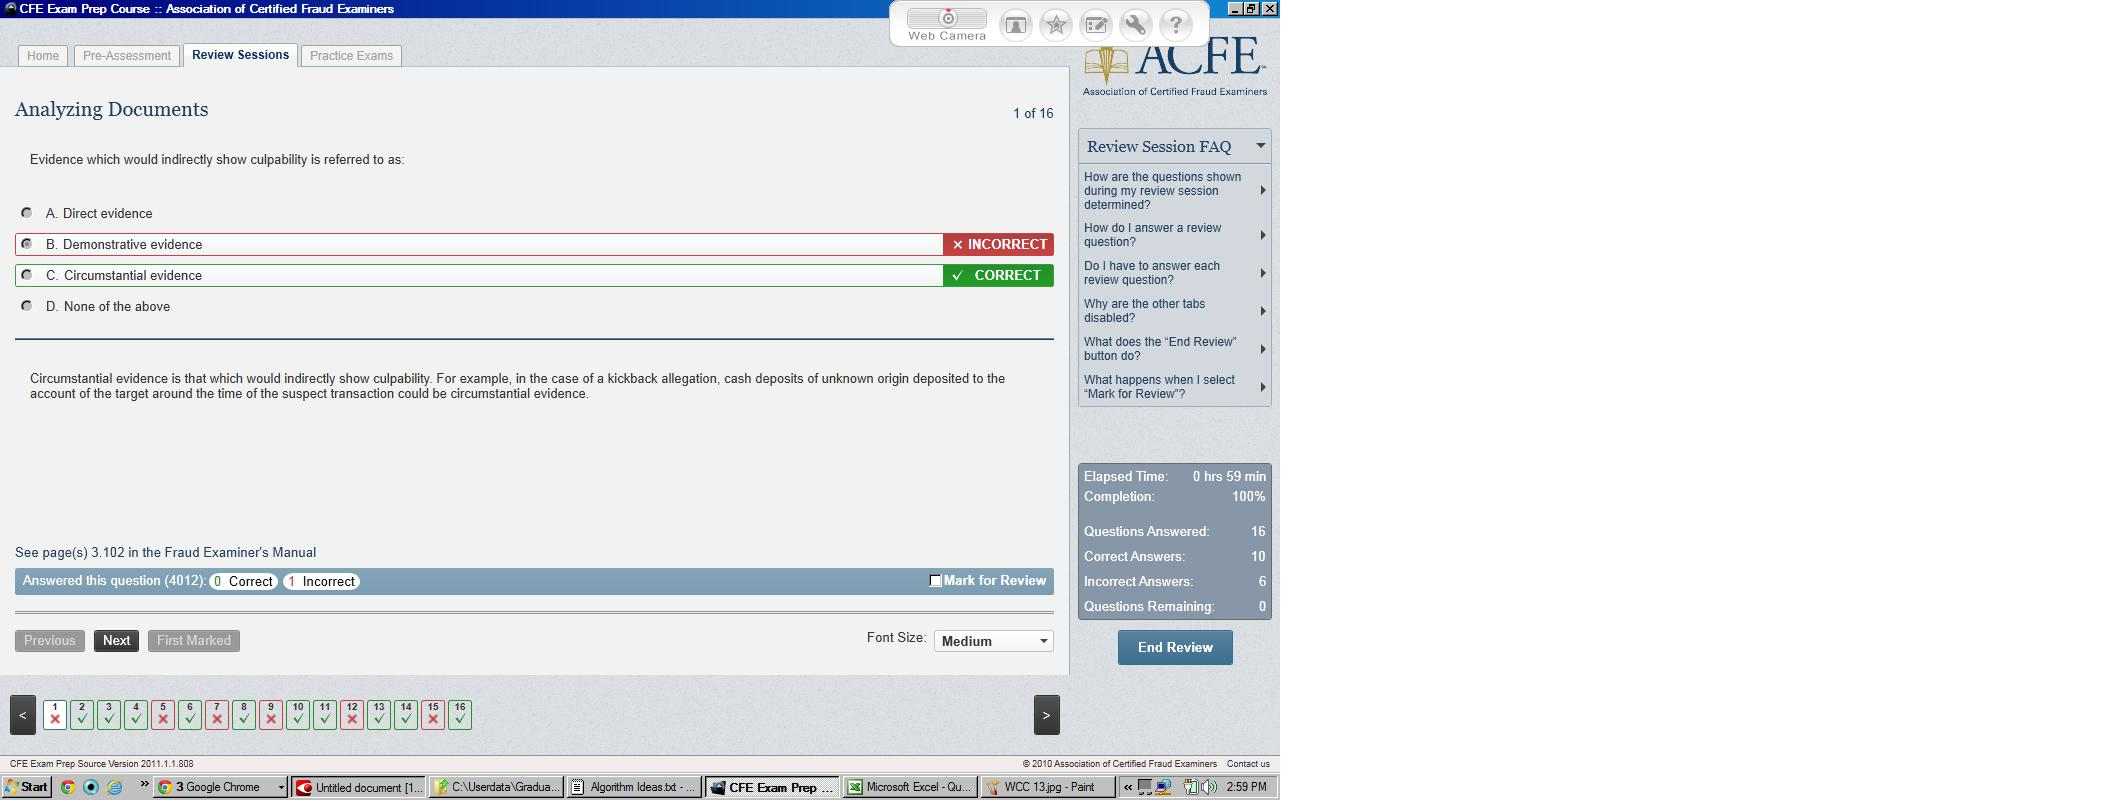
\includegraphics[width=200mm]{study_package_screen_shot.jpg}
\caption{Embedded Practice Question}
\label{fig:study_package_screen_shot}
\end{figure}

\begin{figure}
\centering
\vspace{2.0in}
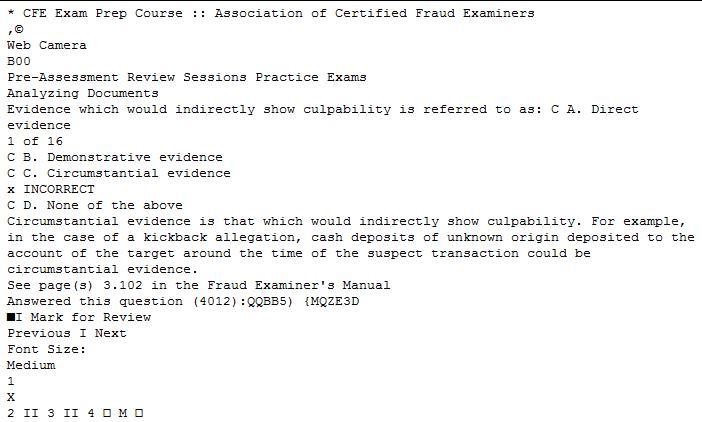
\includegraphics[scale=0.75]{study_package_unformatted_text.jpg}
\caption{Converted, Unscrubbed Practice Question}
\label{fig:study_package_unformatted_text}
\end{figure}

\begin{figure}
\centering
\vspace{2.0in}
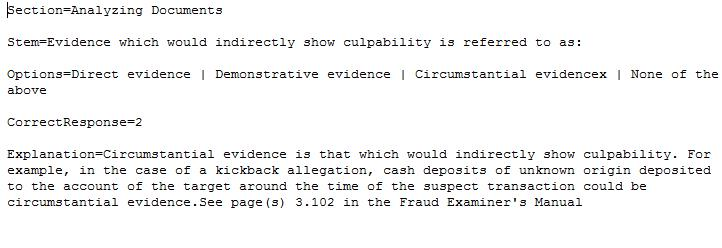
\includegraphics[scale=0.75]{study_package_formatted_text.jpg}
\caption{Scrubbed Practice Question}
\label{fig:study_package_formatted_text}
\end{figure}

The other main component of the prep package is the database of 1,500 questions embedded in the study package software.  The extraction of these questions from the software was an involved, multi-step process.  First, a screenshot file, as shown in Fig.~\ref{fig:study_package_screen_shot} \cite{acfe_study_package_2011},  was created for each question.  Second, optical character recognition (OCR) software was used to convert the graphic screen shot files into text files, as shown in Fig.~\ref{fig:study_package_unformatted_text}.  Unfortunately, the important data needed for each question was intermingled among nonsensical overhead text in each of these text files.  So, a custom program was created to parse these text files, remove the unnecessary data, and decompose each question into its component parts --- topic, question stem, options, correct answer, and explanation --- as shown in Fig.~\ref{fig:study_package_formatted_text}.  Finally, these files were manually reviewed and edited to ensure proper format for the agent.  The product of this process was a collection of 1,500 text files, one for each practice exam question, and each containing name-value pairs for the relevant question fields named above.




%\subsection{CFE Agent Design}
\section{CFE Agent Design}

The CFE Agent is an object-oriented program written in Java.  It takes as input a collection of question files and produces as output a sequence of answers which are, in turn, compared against the corresponding correct answers in order to calculate a score.  There are five principal elements to the design of the CFE Agent --- the CFE manual, the question profile, the algorithm set, algorithm profile data, and the algorithm-selection algorithm.

%\subsubsection{Question Profile}
\subsection{Question Profile}

After having reviewed the entire database of questions in the study package, it was determined that there are certain characteristics certain questions share in common.  This was thought to be a natural way of partitioning the questions according to a crude ontology each class of which could serve as a means for optimizing an algorithm for the questions of that class.  For example, one of the most obvious of these characteristics is whether the question is a true-false question or a multiple-choice question.  And if the question is true-false, does it include any of the following terms:  ``always'', ``never'', ``must'', or ``only''?  On the other hand, if a question is multiple choice, is its last option, ``All of the above''?  Some other criteria discovered that are worth noting are whether the question includes options with more than four words in it, whether the question contains the word ``except'', and whether the question's last option is ``None of the above''.

%\subsubsection{Algorithm Set}
\subsection{Algorithm Set}

Various algorithms were developed and incorporated into the model.  The system currently employs nine custom algorithms that utilize natural language processing, information retrieval, and general test-taking techniques.  Descriptions of a few example algorithms are given below:

\subsubsection{Max Joint Probability Algorithm}

This algorithm considers only the possible answers, treating each as a sequence of words whose joint probability is to be calculated.  It calculates this joint probability for each option by finding the probability of each word among the words of the manual section from which the question was drawn (indicated by topic) and by applying the simplifying assumption of independence between words.  The joint probability, then, is simply calculated as the product of the probabilities of the individual words of the option, normalized for the number of words (so that short answers are not over-weighted).  The algorithm selects the option with maximum joint probability.

\subsubsection{Max Frequency Algorithm}

The Max Frequency Algorithm simply counts up the total number of times each answer option is encountered in the manual section from which the question was drawn and selects the option whose tally is the largest.  Unlike the Max Joint Probability Algorithm, the frequencies are based on occurrences of entire phrases, not on the counts of individual words within them.

\subsubsection{False Select}

This algorithm applies only to true-false questions, simply selecting false, always.  Remarkably, this algorithm proved extremely effective for such questions that have ``must'', ``always'', ``only'', or ``never'' in the stem, achieving an astonishing 78.7\% accuracy rate on this class of questions.  The remarkable success of such a simple algorithm is an indication of the effectiveness of gaming strategies on certain questions, but also an indication of weaknesses in the way certain questions on this exam are designed.

\subsection{Algorithm Profile Data}

The algorithm profile data is a table showing accuracy each algorithm on each question question profile, tabulated from running every algorithm on every question in a training set of 1,300 question selected from the battery of 1,500 questions.  For each of these questions, a profiler component performed the following steps:  First, determine the question profile.  Second, execute each algorithm on the question, recording whether each algorithm produced the correct answer.  Finally, summarize the results.  A portion of this summary data is shown in Fig.~\ref{fig:profile_data_training_set}

\begin{figure}
\centering
\vspace{2.0in}
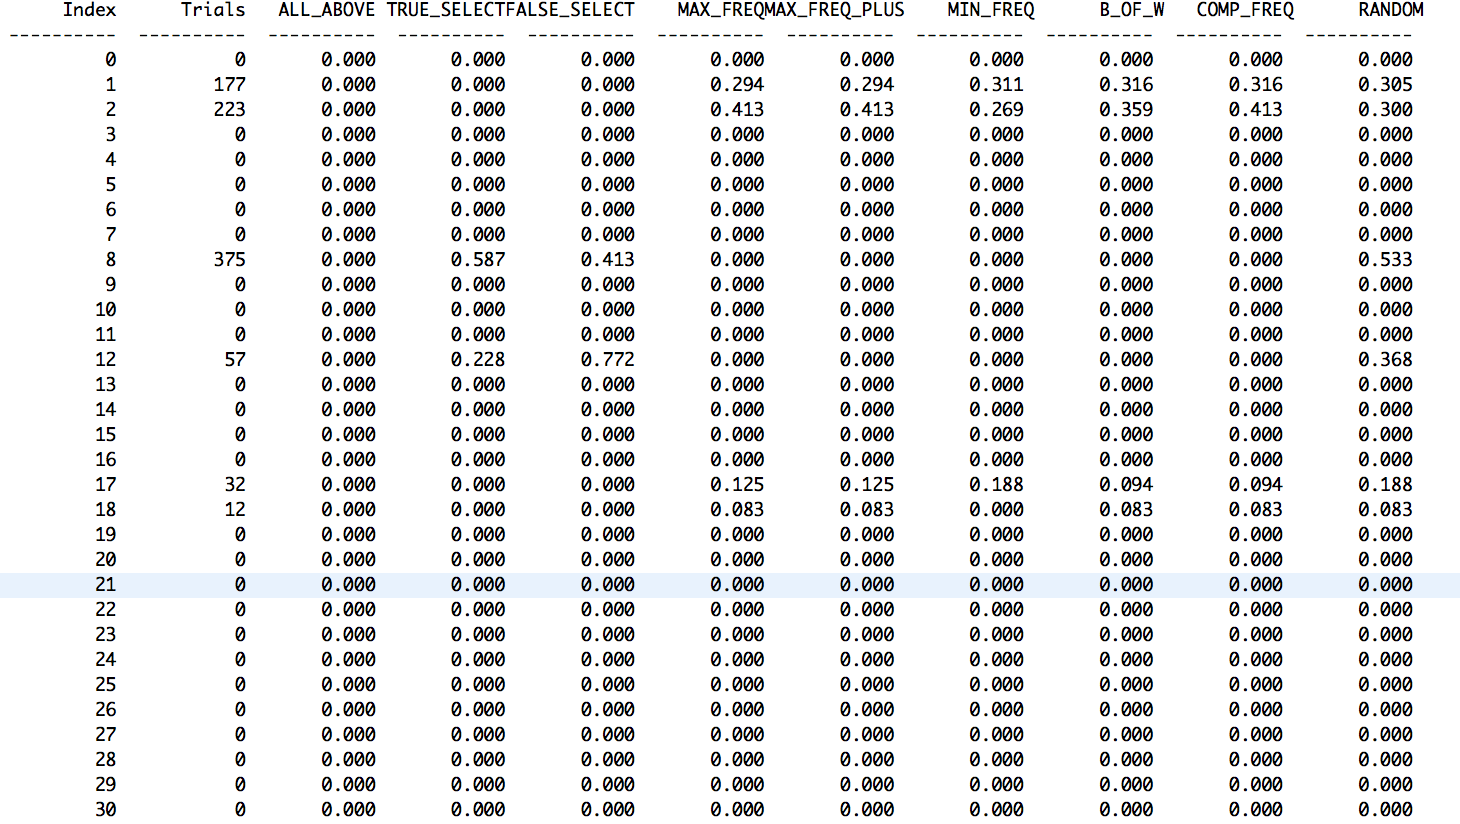
\includegraphics[scale=0.25]{profile_data_training_set.png}
\caption{Training Set Profile Data}
\label{fig:profile_data_training_set}
\end{figure}

%\subsubsection{The Selection Algorithm}
\subsection{The Selection Algorithm}

The selection algorithm is the procedure for selecting the proper algorithm to apply to a given question.  It is based on the algorithm profile data described above.  For a given question in the 200-question test set, the CFE Agent chooses the algorithm with the highest accuracy rate for questions in the training set with the same profile.

%\subsection{CFE Agent Demo}
\section{CFE Agent Demo}

This section outlines a walkthrough of the execution of the CFE Agent for a very short exam, consisting of only four questions.  Despite its short length, it should provide a good idea of the basic mechanics of the agent.  

Fig.~\ref{fig:cfe_agent_startup} shows the startup of the agent.  The name of a configuration file is passed in as a command line parameter to the program.  This file provides a number of settings for the execution environment, including the mode (interactive vs. batch), the name of the exam file, and log detail level.  In this demo, the agent is executing with full detail so that it is easier to understand what is happening under the covers for each question.

The detail logging shows that one of the first things the CFE Agent does when it starts up is construct an internal representation of the CFE Manual.  This internal representation is in the form of a graph, each of whose nodes represents a section of the document.  More specifically, the graph is a tree whose root node represents the entire manual, which in turn possesses links to child nodes each representing one of the four main sections of the manual (Financial Transactions and Fraud Schemes, Law, Investigation, and Fraud Prevention and Deterrence) each of which in turn possesses child nodes representing sub-sections to those sections, and so on.  Each node stores information about the section it represents in addition to the text itself, including a hash table for word counts, sub-subheadings, et cetera.  This information facilitates the text analytic computations the agent performs as it answers questions on the exam.  It should be noted that much of the basis of this tree data structure is based on the items listed in the manual’s table of contents, and for even finer-grained detail nodes, on text features within the corpus itself.  (That is, lines of text consisting of all capital letters terminating in carriage return generally denote a sub-section of text).  Finally, in addition to the tree data structure, the internal representation of the manual includes additional data structures mapping the text of the manual for optimizing access to particular manual subsections.

\begin{figure}
\centering
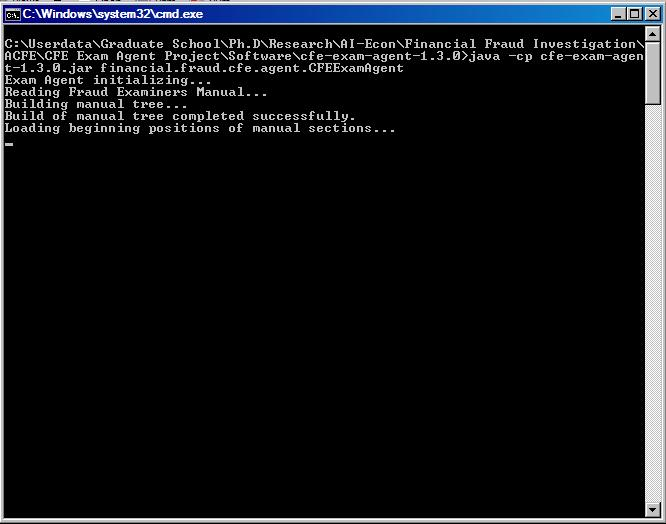
\includegraphics[scale=0.75]{screen_shot_1.jpg}
\caption{CFE Agent Startup}
\label{fig:cfe_agent_startup}
\end{figure}


In Fig.~\ref{fig:cfe_agent_startup_completed}, the screen shows the completion of the startup sequence of the CFE Agent.  First, the CFE Agent gives a line-by-line report showing the nodes loaded into the tree data structure.  Then, it shows some additional configuration information showing the exam file, execution mode, and runtime status.  At this point, the CFE Agent is ready to begin the exam.

\begin{figure}
\centering
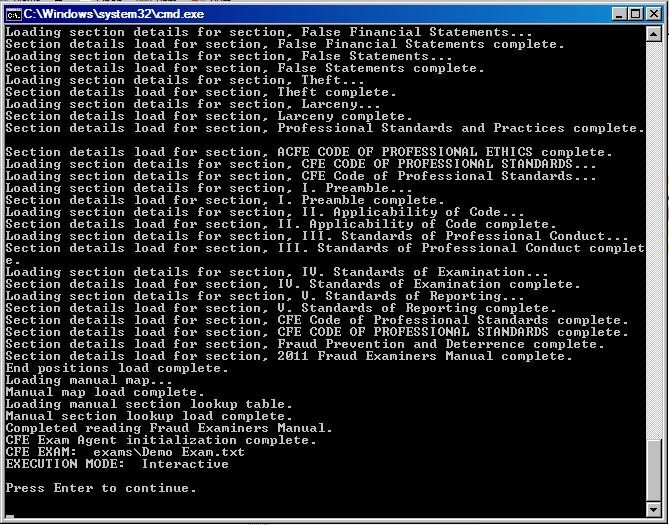
\includegraphics[scale=0.75]{screen_shot_2.jpg}
\caption{CFE Agent Startup Completed}
\label{fig:cfe_agent_startup_completed}
\end{figure}

In Fig.~\ref{fig:first_question}, the first question of the exam is shown along with four possible answers.  After the user presses return, the CFE Agent selects the optimal algorithm for that particular question and executes it.  

\begin{figure}
\centering
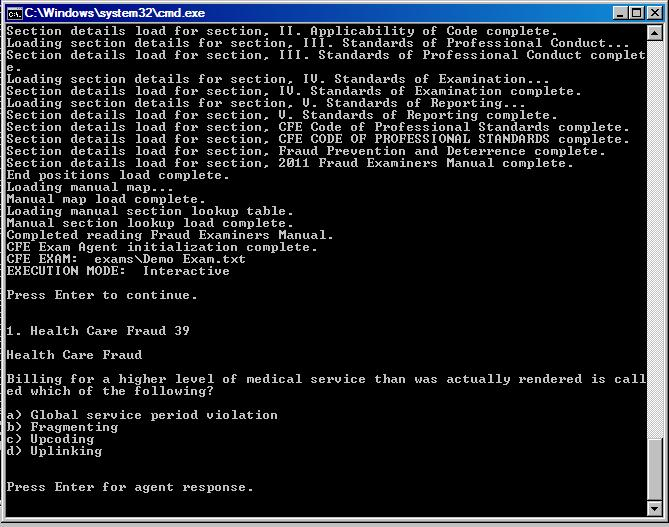
\includegraphics[scale=0.75]{screen_shot_3.jpg}
\caption{First Question}
\label{fig:first_question}
\end{figure}

Fig.~\ref{fig:first_question_completed} shows log detail for the CFE Agent as it attempts to choose the correct answer for the first question.  First, as described in the discussion of the question profile, the agent makes an assignment to a question profile category based on some key features of the question, (whether it's a true-false question, a question at least one of whose options contains more than 4 words, et cetera).  Once it assesses the question profile, it chooses an algorithm which based on prior experience exhibits maximum accuracy on questions having the same profile.  For this question, the profile assignment is category 2, meaning the question has been categorized as a ``definition'' question – essentially one which attempts to test for knowledge of domain-specific vocabulary.  The experience data of the Agent indicates the best performing algorithm is the Max Frequency algorithm, which when applied for this question results in the selection of choice c, the correct answer.

\begin{figure}
\centering
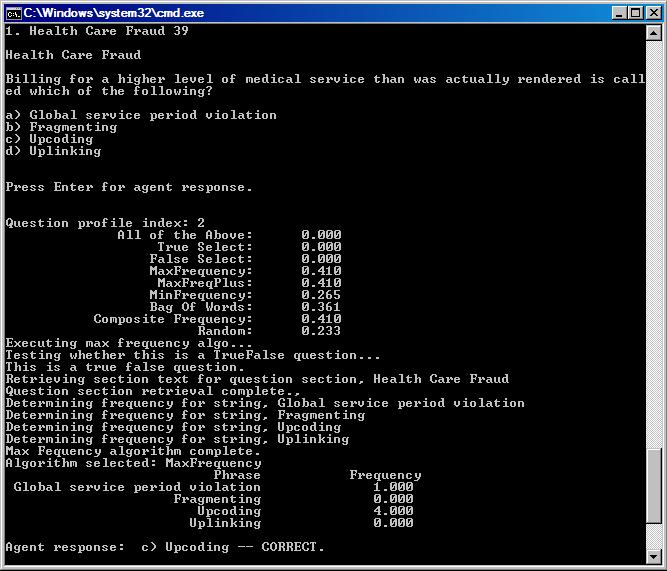
\includegraphics[scale=0.75]{screen_shot_4.jpg}
\caption{First Question Completed}
\label{fig:first_question_completed}
\end{figure}

Fig.~\ref{fig:second_question} shows the CFE Agent answer the second question.  This question appears to be similar to the first in that it also earns a category assignment of 2, meaning it is another ``definition'' question.  By the same experience-based reasoning as in the first question, the agent applies the Max Frequency algorithm and selects answer a, the correct answer.

\begin{figure}
\centering
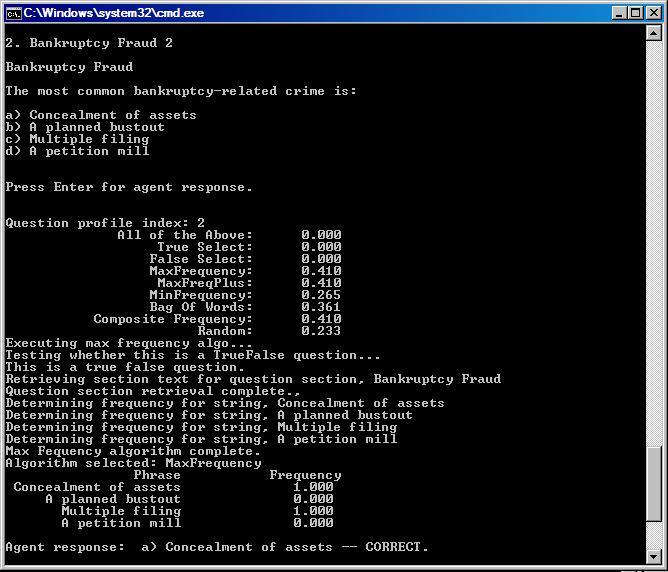
\includegraphics[scale=0.75]{screen_shot_5.jpg}
\caption{Second Question}
\label{fig:second_question}
\end{figure}

Fig.~\ref{fig:third_question} shows an attempt at the third question.  However, this time the agent is not successful at choosing the right answer.  Again, it assigns this question to the same category as the two prior questions and uses the same Max Frequency algorithm, but it is led astray by the fact that the fourth option, ``cost'' is a common word whose frequency in the section corpus is over-weighted relative to the other options for this question.  This is an example where the current level of sophistication of the agent is insufficient to correctly answer questions one of the options may consists of a word or phrase that might be over-represented in the corpus.  Further work will need to be done to develop the natural language processing algorithm to compensate for this over-weighting, while preserving its relative success on other questions in the same category.

\begin{figure}
\centering
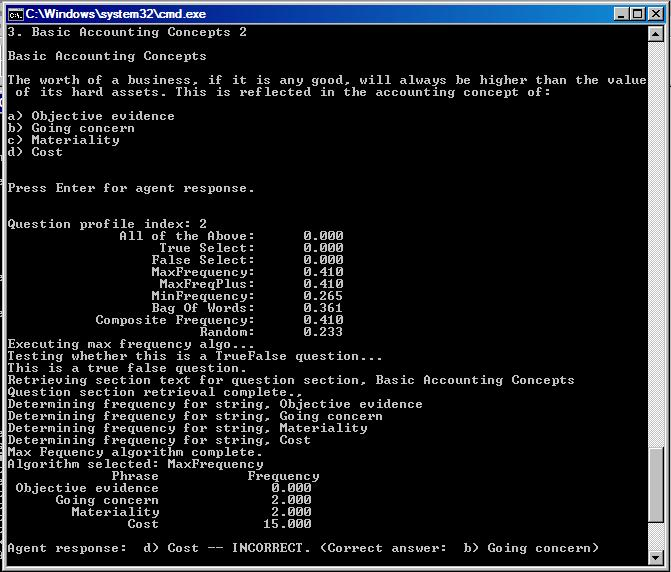
\includegraphics[scale=0.75]{screen_shot_6.jpg}
\caption{Third Question}
\label{fig:third_question}
\end{figure}

Fig.~\ref{fig:final_question_and_termination} shows the final question, which is one of a different type --- an ``All of the Above'' question.  Here, the CFE Agent chooses an algorithm appropriately called ``All of the Above'' because it simply selects ``All of the Above'' whenever its an option.  (As shown in the data table, this algorithm has a remarkable 86\% success rate, lending one to question certain aspects of the CFE Exam’s design, as mentioned earlier.)  The agent applies this algorithm and gets the answer correct.  Finally, the agent terminates.

\begin{figure}
\centering
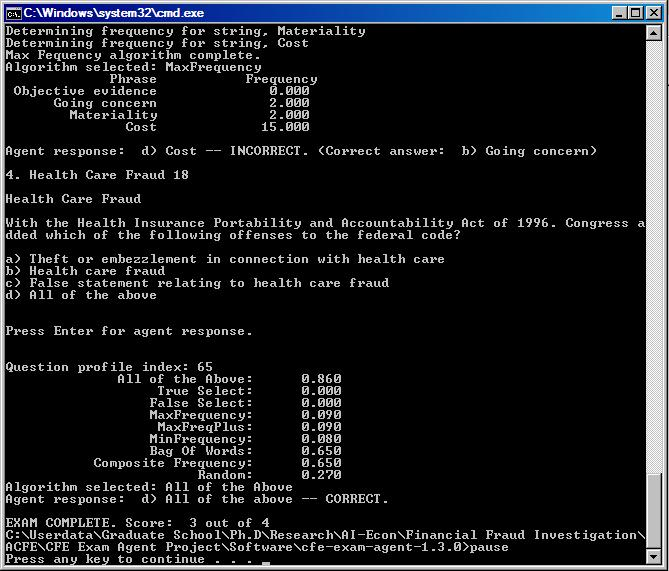
\includegraphics[scale=0.75]{screen_shot_7.jpg}
\caption{Final Question and Termination}
\label{fig:final_question_and_termination}
\end{figure}


%\subsection{CFE Agent Results - A Good Start}
\section{CFE Agent Results - A Good Start}

A detailed look at the performance of the agent on the entire battery of 1,500 questions, assuming the agent employs the most accurate algorithm for each question, given its profile, shows the agent demonstrates promising, statistically significant performance.  Consider the question of whether the agent actually performed any better than random guessing.  For true-false questions, random guessing would be expected to yield an accuracy rate on the of approximately 50\%.  (Given there are a relatively large number of true-false questions (506), it is reasonable to assume the experimental accuracy rate should be very close to this theoretical value.)  Likewise, for multiple-choice questions with four options, random guessing should yield an accuracy rate of approximately 25\%.  (Again, for the same reason as for true-false questions, the experimental accuracy should be close to the theoretical expected value.)  However, the empirical data shown in Fig.~\ref{fig:results_for_true_false_questions} and Fig.~\ref{fig:results_for_multiple_choice_questions} indicates that for true-false questions, the observed accuracy rate is over 58\% on this training set, giving a z-score of over 3.729 (the z-score for a p-value of 1\% is 2.575), and that for multiple-choice questions, the accuracy rate is just over 47.8\%, giving a z-score of 16.67.  For both classes of questions, then, the null hypothesis of performance consistent with random guessing is rejected by a large margin at the 99\% significance level.  


\begin{figure}
\centering
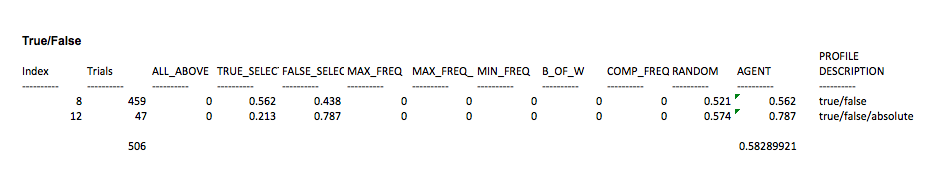
\includegraphics[width=130mm]{true_false_results_1500.png}
\caption{Results for True-False Questions}
\label{fig:results_for_true_false_questions}
\end{figure}

\begin{figure}
\centering
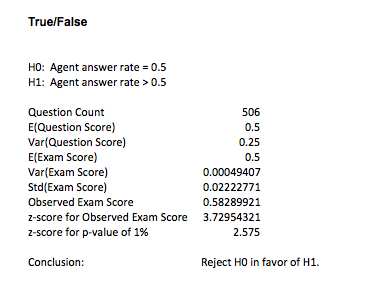
\includegraphics[scale=0.75]{true_false_hypothesis_test_1500.png}
\caption{Hypothesis Test for True-False Questions}
\label{fig:hypothesis_test_for_true_false_questions}
\end{figure}

\begin{figure}
\centering
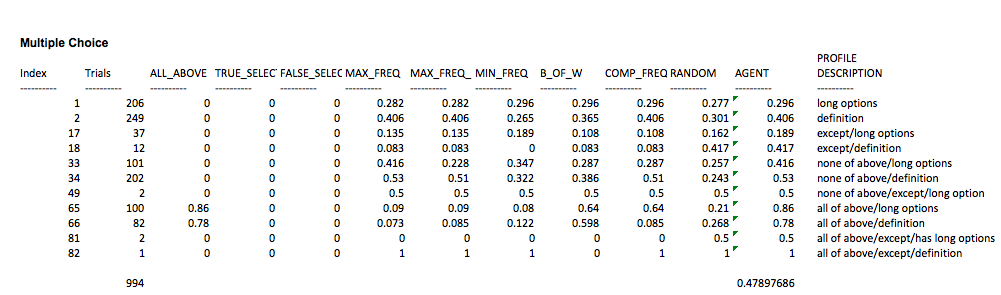
\includegraphics[width=130mm]{multiple_choice_results_1500.png}
\caption{Results for Multiple-Choice Questions}
\label{fig:results_for_multiple_choice_questions}
\end{figure}

\begin{figure}
\centering
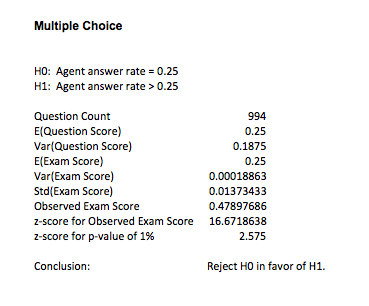
\includegraphics[scale=0.75]{multiple_choice_hypothesis_test_1500.png}
\caption{Hypothesis Test for Multiple-Choice Questions}
\label{fig:hypothesis_test_for_multiple_choice_questions}
\end{figure}
 

The above analysis covers the entire battery of 1,500 questions.  However, in developing our agent, this battery was broken into two subsets - a training set consisting of 1,300 questions and a test set consisting of 200 questions.  The idea here is to utilize the training set to determine the optimum algorithm for each profile (that is, the one whose accuracy is highest), and then to apply that knowledge on the test set by applying the best algorithm for each question, based on its profile.  The process of breaking the collection of questions up into a training set and test set was done via a programmatic procedure that selected a random, proportionate selection of questions for each CFE-exam subtopic.  Fig.~\ref{fig:version_1_training_set_results} shows the results for the training set are comparable to those for the 1,500-question battery, as should be expected.  Using this data, the CFE Agent was executed on the 200-question test set, where it answered 98 correct, or 49\%.  Although this is short of passing, it's an encouraging start, and provides a good baseline for subsequent versions of the agent.

\begin{figure}
\centering
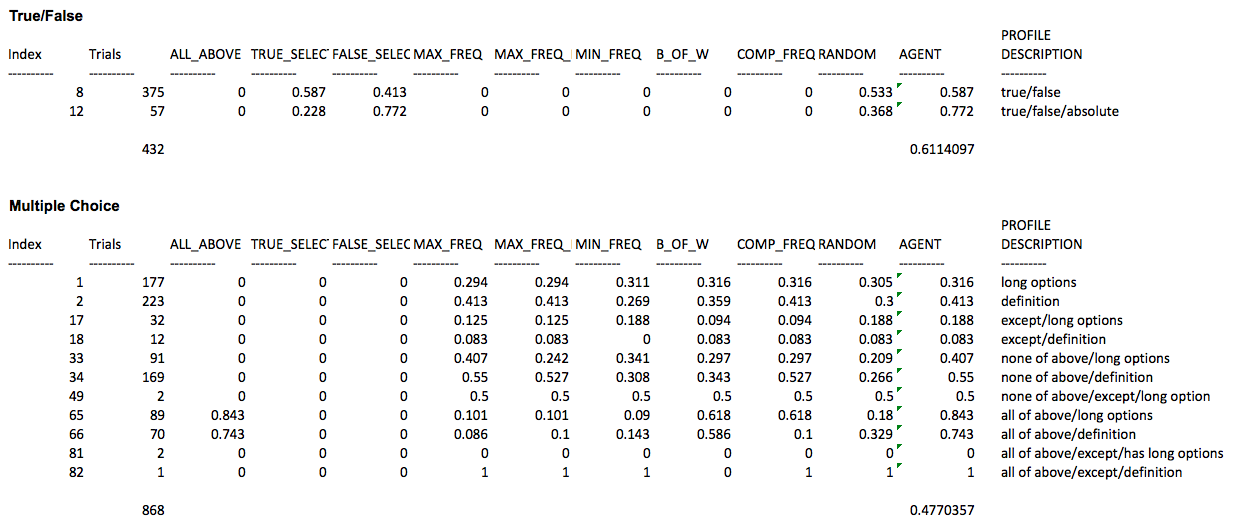
\includegraphics[width=130mm]{version_1_training_set_results.png}
\caption{Results for Multiple-Choice and True-False Questions on 1300-Question Training Set}
\label{fig:version_1_training_set_results}
\end{figure}

Finally, it should also be pointed out that during development of later versions of the agent, it was noticed that an important question feature had been overlooked in the original analysis -- the notion of a ``not'' question.  An example of a not question is:  ``Which of the following is NOT one of the major standards of generally accepted accounting principles?''.  It was found to be necessary to break out questions of this variety from other questions that were otherwise of the same type, but did not include the ``NOT'' term.  Thus, the analysis was completed once more on the training set, showing the following results in Fig.~\ref{fig:version_1_training_set_results_not}.  It should be noted from this table, for example, that among the 223 questions formerly  categorized as ``definition'' questions, 40 are now categorized as ``definition/not'' questions.  The same phenomenon occurs for other categories, as well.  

\begin{figure}
\centering
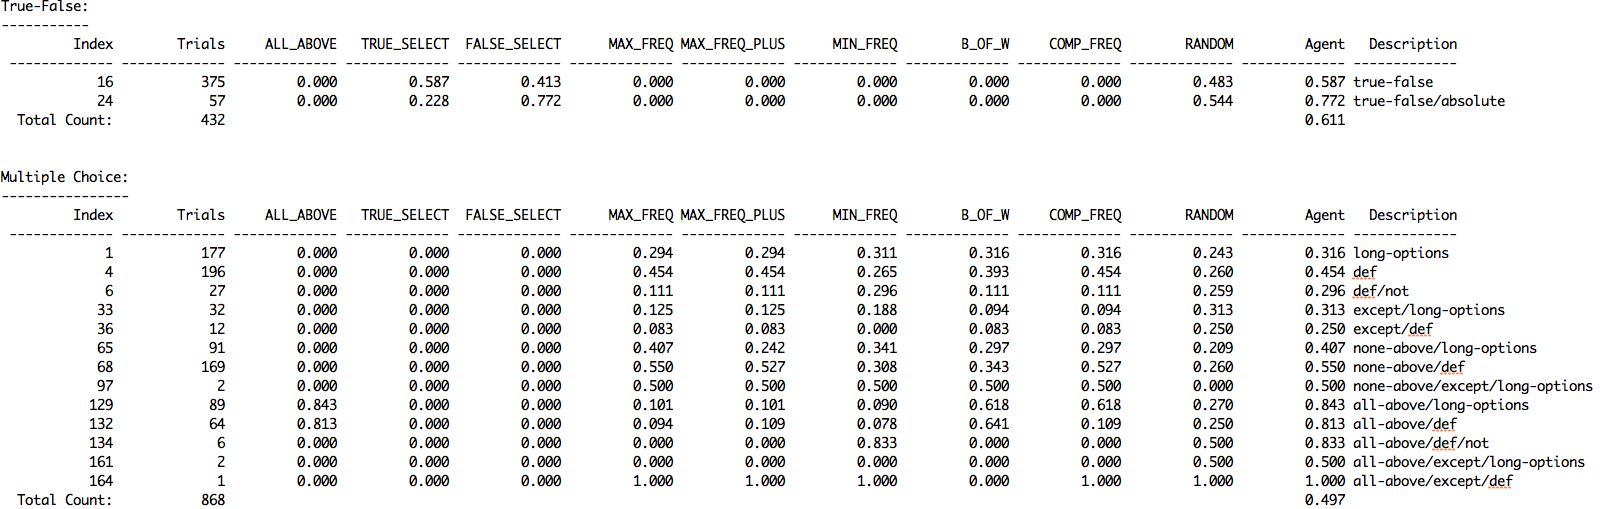
\includegraphics[width=130mm]{version_1_training_set_results_not.png}
\caption{Training Set Results with NOT Feature Breakout}
\label{fig:version_1_training_set_results_not}
\end{figure}



 % chapter 3 - Intelligent Agent - Version 1
%%%%%%%%%%%%%%%%%%%%%%%%%%%%%%%%%%%%%%%%%%%%%%%%%%%%%%%%%%%%%%%%%%% 
%                                                                 %
%                            CHAPTER FOUR   - A More Sophisticated Agent- Version 2            %
%                                                                 %
%%%%%%%%%%%%%%%%%%%%%%%%%%%%%%%%%%%%%%%%%%%%%%%%%%%%%%%%%%%%%%%%%%% 
 
\chapter{Version 2 -- A More Intelligent Agent}

In this chapter, we describe Version 2 of the CFE Agent, enhanced with improved algorithms for locating the relevant section(s) of the CFE Manual for each question.  Version 1 of the CFE Agent is limited to coarse-grained sections as defined by the question sections of the CFE Exam and Manual.  Unfortunately, these sections of the manual are effectively so large, it's difficult for the agent to drill down to the text \emph{directly} related to a given question.  For intellectual-property-theft questions, for example, the ``Theft of Intellectual Property" section of the manual is 89 pages long.  For any question on this topic, pulling the entire section of the CFE manual will assure that the answer sought lies somewhere within our target document.  But with 89 pages of text in the section, we might still get the answer wrong.  Version 2 refines the filtering algorithm to help avoid this problem.



This chapter is laid out as follows:  First, we review the basic elements of Information Retrieval, the branch of AI dealing with retrieving documents from within a large collection related to an information need.  Next, we explore the open source software, Lucene, an Apache sofware program that provides information retrieval functionality.  This package was used in the implementation of Version 2 of the CFE agent.  Then, we look at the method used to break up the CFE manual into finer-grained sections, leveraging the table of contents and text metadata as means for dividing up the text along reasonable semantic lines into a collection of documents.  And finally, we present the analysis performed of a set of algorithms implemented in Version 2 using these information retrieval tools and this document collection.

One note before proceeding:  The terms, ``training set" and ``test set" are used throughout this chapter in reference to the battery of questions against which the algorithms discussed below were applied.  Indeed, we talk repeatedly about testing our algorithms against the training set, specifically. It is important to note here that ``training set" is a term of convenience in this chapter, and not one that should be taken to suggest a set for which we've optimized parameters vis \`a vis machine learning.  In fact, the algorithms we discuss in this chapter involve no training, per se, and so, it is perfectly valid to measure or test the performance of each of these algorithms against the ``training set".   (In chapter 5, however, we \emph{do} employ machine learning, and the training set and test set are used according to their conventional definition.)  Lastly, it should be mentioned that at the end of this chapter, we use the performance of each algorithm on the questions of the training set to determine the optimal algorithm to use on each question in the test set in order to measure overall performance of Version 2 of the agent.

Finally, before moving any further, during the development of Version 2, a deeper review of the definition-type questions was in order.  Some questions were re-classified according to finer grained criteria, including the following:  Nine questions were reclassified as ``I, II, III, and IV" type.  Six questions for which ``Any of the Above" was an option were re-classified as ``All of the Above" type.  There were 26 questions whose answers weren't derived from the Fraud Examiners Manual but instead from a different text, The Corporate Fraud Handbook.  Finally, five questions were re-classified as ``NOT" questions.  After reclassifying these questions, we were left with 150 definition questions in our training set upon which to base our algorithm performance analysis, reduced from our original 196 questions used for Version 1.


\section{Information Retrieval}

Information Retrieval (IR) is the branch of AI dealing with the creation of software that retrieves documents of an unstructured nature from among a large collection of documents in response to an information need expressed as a natural language query \cite{manning_2008_introduction_ch1}.   A document is a unit of data, typically unstructured or semi-structured, and typically expressed in natural language.  (One of the fundamental questions to consider in IR is how to define a document - a sentence? a paragraph? a chapter?  The answer typically depends on the nature of the problem domain.)  A document collection is simply a collection of such documents, as defined above.  Finally, a vocabulary, $V=\{t_1,t_2,t_3,...,t_n\}$ is the set of all terms over which the contents of the documents are defined.

\subsection{Boolean Retrieval}

Boolean information retrieval is based on the idea of dividing up the document collection into two sets for each query - one set of documents which meets the requirements of the boolean query and the other set whose documents does not.  Boolean queries are structured as conjunctions of disjunctions; that is, of the form of query, $q$, where

%\begin{gather*}
%q = (W_i \lor W_k \lor ...) \land ... \land (W_j \lor W_s \lor ...) \\
%\textrm{where}\ W_i = t_i, W_k = t_k, W_j = t_j, W_s = t_s, \\
%\textrm{or}\ W_i = NON\ t_i, W_k = NON\ t_k, W_j = NON\ t_j, W_s = NON\ t_s \\
%\text{where $t_i$ means that $t_i$ exists in the document and $NON\ t_i$ means it does not}
%\end{gather*}

\begin{equation}
q = (W_i \lor W_k \lor ...) \land ... \land (W_j \lor W_s \lor ...) \\
\end{equation}
where $W_i = t_i, W_k = t_k, W_j = t_j, W_s = t_s,$ or $W_i = NON\ t_i, W_k = NON\ t_k, W_j = NON\ t_j, W_s = NON\ t_s$ and where $t_i$ means that $t_i$ exists in the document and $NON\ t_i$ means it does not \cite{wiki:boolean_retrieval}.

%q = (Wi OR Wk OR ...) AND ... AND (Wj OR Ws OR ...)
%
%where Wi=ti, Wk=tk, Wj = tj, Ws = ts, or Wi = NON ti, Wk = NON tk, or Wj = NON tj, or Ws = NON ts, 
%
%where ti indicates the term ti is present in the doucument and NON ti indicates it is not.

\subsubsection{Term-Document Incidence Matrix}

Boolean retrieval may be  implemented using a data structure called a term-document incidence matrix, $A$, where $A$ is a two-dimensional array in which the $i$th row denotes the $i$th document in the document collection and where $j$th column denotes the $j$th term in the vocabulary, and where $A[i,j] = 1$ if the term, $i$ exists in the document, $j$, and 0 otherwise.  Based on $A$, the processing of a query involves finding those documents for which there is a 1 in each of the rows corresponding to the terms of the query \cite{manning_2008_introduction_ch1}.  

A significant pitfall of this method is that it requires a vast amount of memory.  Consider an example consisting of 1 million documents and a vocabulary of 500,000 words.  Then, the size of the matrix is 50 trillion (1 million x 500,000).  This matrix is also highly sparse since any given document has on average a small number of words relative to the size of the vocabulary.  Suppose, for example, each document has 1,000 words.  Then, for each document, among the 50,000 elements in its corresponding row of the matrix, only 1,000 (2\%) are non-zero \cite{manning_2008_introduction_ch1}.	

\subsubsection{Inverted Index}

An alternative implementation for boolean retrieval utilizes an inverted Index -- a hash table in which the keys are the terms in the vocabulary and the value is a linked list of all of the identifiers for those documents in which that term appears.  This technique exploits the sparsity of the term-document matrix -- requiring memory only for those elements in which $A(i,j) = 1$ \cite{manning_2008_introduction_ch1}.


\subsection{Ranked Retrieval}

Boolean retrieval has the unfortunate drawback of returning a set of documents in response to a query as a set of equally ranked units through which the user must sift in order to find the information sought \cite{manning_2008_introduction_ch6}.  Sometimes, this sifting can be sizable task depending on the number of documents returns from the boolean query.  Ranked retrieval, on the other hand, is IR in which documents are ranked according to a score that measure the degree of similarity between the query and the terms of the document and in which documents are returned in decreasing sorted order of this score \cite{manning_2008_introduction_ch6}.  

The Vector Space model (VSM) \cite{manning_2008_introduction_ch6} is one approach to ranked retrieval, and is based on representing the documents in the collection and the query as vectors and where documents are scored according to a measure of similarity between their vector representations and that of the query.  There are a number of measures, or weights, that are typically incorporated into a vector representation as discussed below.

The log of the term frequency, $\textrm{log}_{10}(tf)$ is a measure of the number of occurences of a particular term in the document.  (The log is used as opposed to the term frequency, itself, in order to dampen the effect for each additional occurrence of a term.)  The log-frequency weight of term, $t$ in document, $d$ is given by \cite{manning_2008_introduction_ch6}:

\begin{equation}
w(t,d) = 1 + \textrm{log}_{10}(tf_d), \textrm{where}\ tf_d > 0, 0\  \textrm{otherwise}
\end{equation}

Inverse document frequency is a measure of the relative scarcity of a term in a document relative to the other documents in the collection.  A higher weight is assigned to a term that appears in relatively few documents compared with one that appears in many.  The inverse document frequency, $idf(t)$, can be calculated for each term, t, of the query as follows \cite{manning_2008_introduction_ch6}:  

\begin{equation}
idf(t)  = \textrm{log}_{10}(N/df_t),
\end{equation}

\noindent
where $N$ is the number of documents in the collection and $df_t$ is the number of documents containing term, $t$.  Again, as is the case for term frequency, the log is used here to moderate the effect of the measure.

We can combine these two measures such that for each term, $t$, in each document, $d$, we have \cite{manning_2008_introduction_ch6}:

\begin{equation}
w(t,d) = (1 + \textrm{log}_{10}(tf_d)) \times \textrm{log}_{10}(N/df_t).
\end{equation}

\noindent
The vector representation of a document, $d$, is $\vec{d}$, where

\begin{equation}
\vec{d} =  [w(t_1,d), w(t_2,d), w(t_3,d),...., w(t_n, d)], 
\end{equation}

\noindent
where, as defined above our vocabulary, $V=\{t_1,t_2, ..., t_n\}$.  Note, queries can also be vectorized in the same way.  

In order to measure the relative relevance of document, $d$, to the query, $q$, the vector representations of both $d$ and $q$, $\vec{d}$ and $\vec{q}$, are harnessed to compute a quantitative measure of the level of similarity between the two vectors using the concept of cosine similarity.  Informally, the cosine similarity of two n-dimensional vectors is a measure of the cosine of the angle between them in n-dimensional space.  Normalization of the lengths of the vectors is also incorporated into this calculation to assure that longer documents' weights do not outsize the weights of shorter (but perhaps, similar) documents, (such as the query itself, which is commonly much shorter than the document against which it is compared).  

\begin{equation}
\begin{split}
\textrm{sim}(q, d) & = \dfrac{\vec{q} \cdot \vec{d}}{|\vec{q}||\vec{d}|} \\
 & = \dfrac{\vec{q}}{|\vec{q}|} \cdot \dfrac{\vec{d}}{|\vec{d}|}
\end{split}
%	= q(arrow)/length(q(arrow)) dot d(arrow)/length(d(arrow)) = 
%	= sum(i to length(V))q(i)d(i)/(sum(i to length(V)q(i)\^2))(sum(i to length(V)d(i)\^2))
\end{equation}

\noindent
For a document, $d$ whose length-normalized-vector representation is similar to that of $q$, the angle between its vector and that of $q$ should be small (close to 0), and thus have a cosine near 1.  For those documents not similar to $q$, the cosine measure will tend toward 0, (note that all of the terms in these vector-representation vectors are greater than or equal to 0).  Under the document vectorization approach, the highest $K$ documents are returned in response to a query, $q$, in order of decreasining cosine similarity, where $K$ is an arbitrary figure intended to limit the size of the return set.




\section{Transforming the CFE Manual into a Document Collection}

The CFE Manual is structured as a text book. As such, it is structured hierarchically, as most textbooks are, complete with features embedded in the text that make this hierarchy apparent.  The most obvious feature is the table of contents (TOC) and headings embedded in the text for each of the chapters, sections, subsections, and so on.  In fact, the CFE Manual has a number of tables of contents, including a main table of contents, at the front of the manual, and a set of area-specific TOCs - one for each of the major test areas - Financial Transactions and Fraud Schemes, Law, Investigation, and Fraud Prevention and Deterrence.  Fig.~\ref{fig:cfe_manual_toc} shows a section of the TOC relating to Financial Statement Analysis, a topic contained in the are of Financial Transactions and Fraud Schemes.  The summary TOC combined with the area-specific TOCs combined with text features (capitalized sub-sub-sub section titles within the text itself) were all used to programmatically break up the manual into a hierarchical structure of documents.  Fig.~\ref{fig:document_collection} shows a portion of this document structure, where on the left we see the Bankruptcy Fraud subsection, a subtopic of Financial Transactions and Fraud Schemes, and the breakdown of documents, each of which named according to a numeric identifier and a title corresponding to a title for the subsection, along with indentation showing its level in the document tree.  On the right side, we see the contents of one of the documents covering the subtopic of Bankruptcy Court.  Notice that in each document we have not only the text of the section but also a a title field (Bankruptcy Court), a question section field (Financial Transactions and Fraud Schemes), a path giving the sequence of section titles starting from the root node of the CFE manual hierarchy to the current document, and finally, the stemmed contents of the document, using the Porter Stemmer algorithm.  All of these elements were compiled for each document as possible inputs to algorithms developed downstream for answering questions.  

\section{Lucene -- A Tool for Information Retrieval}

Lucene, \url{https://lucene.apache.org/}, is a highly popular Apache software product that implements IR using a combination of Boolean Retrieval and the VSM \cite{McCandless:2010:LAS:1893016_ch1,McCandless:2010:LAS:1893016_ch2,McCandless:2010:LAS:1893016_ch3,McCandless:2010:LAS:1893016_ch4}.  First, it narrows the document set using boolean retrieval, and then it ranks the remaining documents using VSM.  The algorithms described below were implemented using this tool.  

\begin{figure}
\centering
\vspace{1.0in}
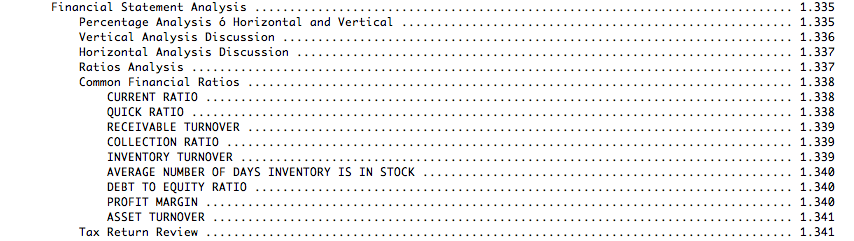
\includegraphics[width=150mm]{cfe_manual_toc.png}
\caption{A section of the table of contents from the CFE Manual}
\label{fig:cfe_manual_toc}
\end{figure}

\begin{figure}
\centering
\vspace{1.0in}
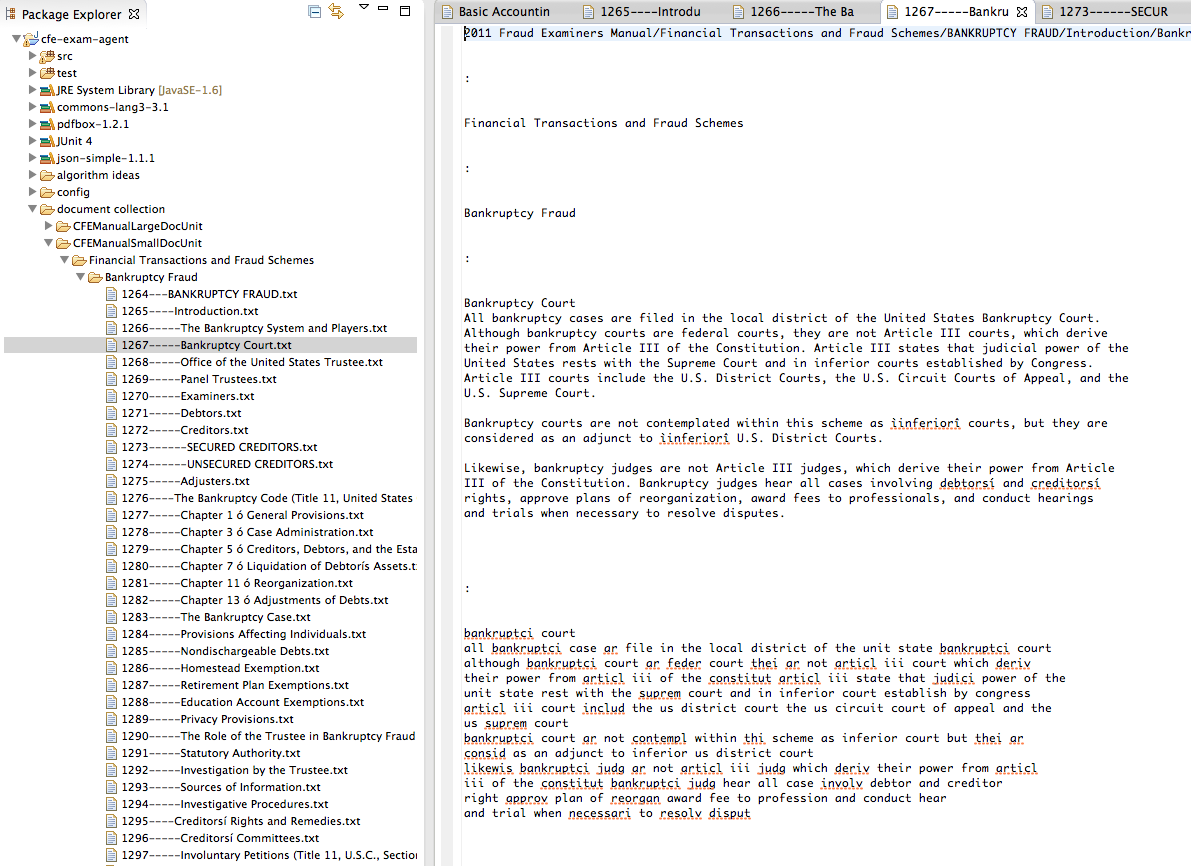
\includegraphics[width=150mm]{document_collection.png}
\caption{The CFE Manual as a Document Collection}
\label{fig:document_collection}
\end{figure}

However, before implementing any algorithms, the document collection into which the CFE manual was decomposed was indexed using the Lucene software.  Indexing is the process of essentially creating files containing the underlying data stuctures required by Lucene's combined boolean retrieval/VSM retrieval algorithm, including an inverted index for the collection and document vectorization data.  In fact, Lucene indexes were created for each question section of the manual, where each question section contains the documents from which an answer to a question pertaining to the material in that section.  When implementing the QA algorithms discussed below, the first step to any of these algorithms was locating the proper index within which to search for relevant documents, based on the exam section/question section that corresponds to the question at hand.  Fig~\ref{fig:lucene_indexes} shows a portion of the lucene indexes created by this process.  Notice that for each question section within each exam section, there are three binary files created by the lucene indexer component that contain the inverted index and document vectorization information required for the query processing component to be used in the algorithms discussed below.

One other thing of note is that as part of this process, the contents field and the title field were stemmed according to the Porter Stemmer algorithm.  Stemming is a form of semantic normalization, where words offering different senses of the same semantic unit are transformed so that they are treated as equivalent during the document scoring computation in the IR process.  For example, different words for run - run, ran, running - are all considered semantically equivalent as a result of stemming.

\begin{figure}
\centering
\vspace{1.0in}
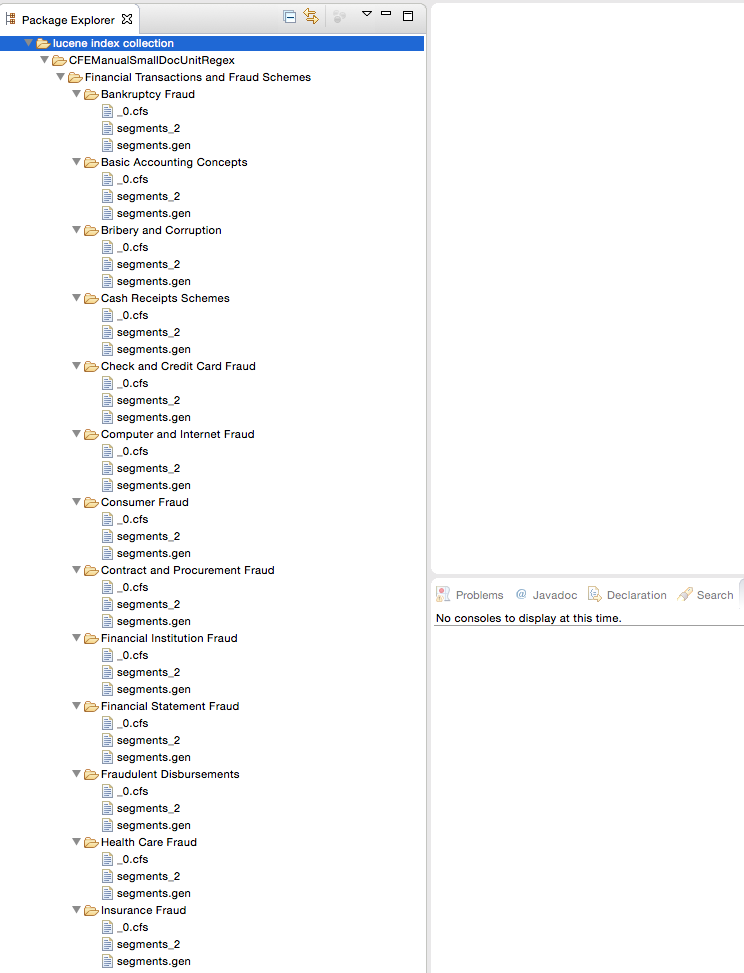
\includegraphics[width=125mm, height=200mm]{lucene_indexes.png}
\caption{Lucene Indexes for a Portion of the Question Sections}
\label{fig:lucene_indexes}
\end{figure}



\section{Analysis Tools for Algorithm Development}

As outlined in prior chapters, the goal of the CFE agent is to answer questions correctly while providing justification for those answers.  As algorithms were developed toward this end, and in particular, as we attempted to refine the accuracy of the agent by making its search functionality more fine-grained, it was determined early in the process that one of the most critical pieces of information was to understand how to target each type of question - What features for a given type of question could be exploited when searching for an answer?  Specifically, how does the answer present itself in the manual to a question of a given type?  Is it contained in a single document, or multiple documents?  Are terms found in the options commonly found in the contents of the document, or are they found in the title?  Depending on the answer, how often is that the case?  Is it always true, or only sometimes?  Tools that aided in this investigation were critical to the development of ``smarter'' algorithms.  

At a macro level, the profiler component, developed for Version 1 of the agent provided an initial analysis tool.  As discussed, it supplied a breakdown of question by macro-features, as well as the success rate of the initial algorithms created for that version.  And here in Version 2, the profiler would be used again.  However, analysis at a greater level of detail was needed.

One component, called the Question Server, was created to at least partially meet this need.  Simple in concept, it would select/pose to the agent only the questions of a particular profile, whether the desired profile be a definition question, a long answer question, and so on.  This provided a means for zero-ing on each type of question in isolation, allowing for various theories and insights to be developed about the best approach for each question.  Fig.~\ref{fig:question_server} shows output from the Question Server for definition/NOT questions, questions whose options are a small number of words (and are thus, typically relate to a definition of a conept), and contain the term, ``not" in the stem, implying the task is to identify the ``odd man out" among the options.

A second component, called the Algorithm Tester, was created on the shoulders of the Question Server, which would demonstate the behavior of each algorithm as it was applied to each question of a given type.  This, too, was instrumental in algorithm development.

\begin{figure}
\centering
\vspace{1.0in}
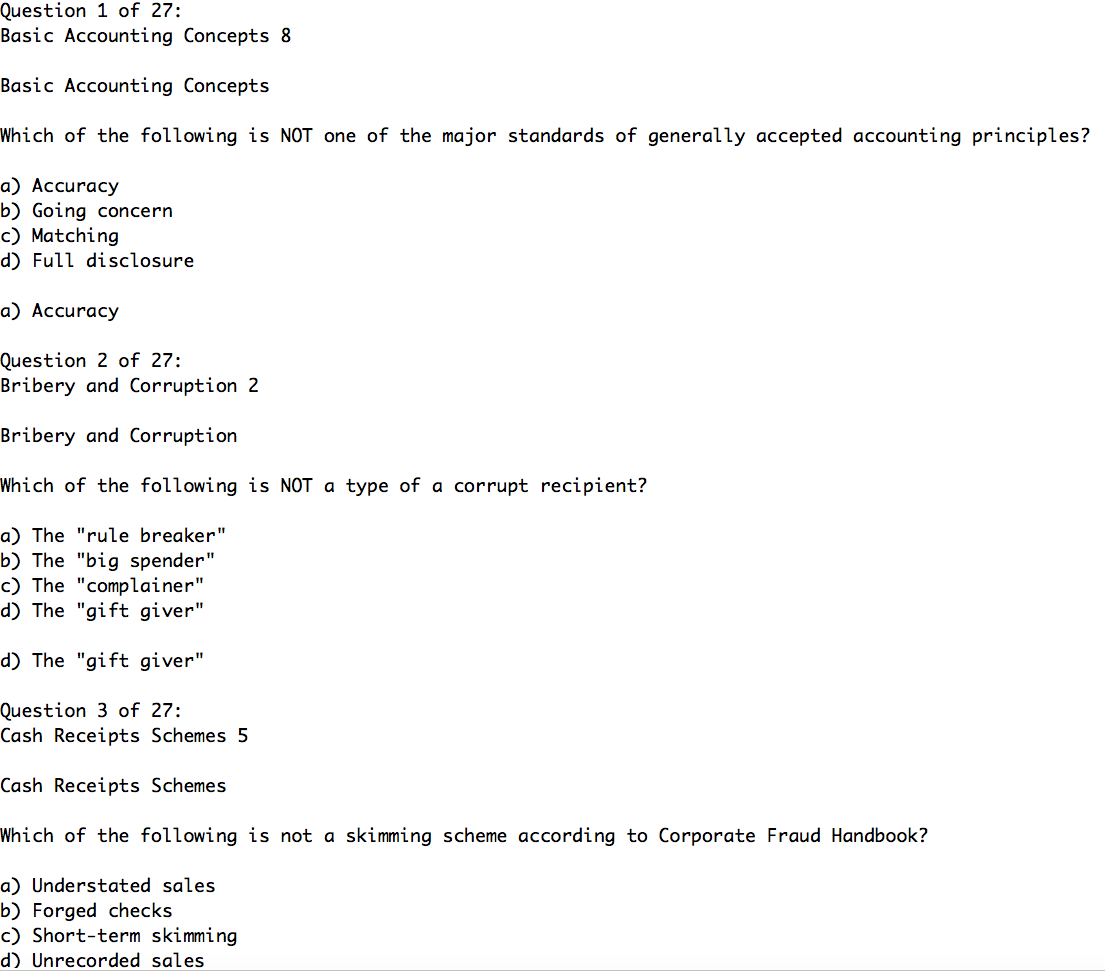
\includegraphics[width=125mm, height=125mm]{question_server.png}
\caption{Question Server Component Targeting Definition/NOT Questions}
\label{fig:question_server}
\end{figure}


\section{Algorithms for Version 2}

This section describes the algorithms implemented for Version 2 of the CFE Agent.  These algorithms rely heavily on IR, as implemented in Lucene.  They also tend to each target a particular question type, in particular, the definition questions - that is, those questions in which each of the options is only a short phrase (consisting of four words or less), and which thus are thought to be most likely the kind of question in which the stem contains a phrase that defines a given concept and the examinee must choose the correct concept from among the four options to which that phrase corresponds.  Given that a large portion of the questions in the training and test sets are some form of this type, more refined algorithms that target this type of question appeared to be a wise choice for where to focus our development efforts.

\subsection{Concept Match Version 1}

Concept Match Version 1 leverages IR on both the question stem and on each of the options in order to determine the one that fits best with the stem.  The essence of the algorithm is to first, conduct an IR query against the document collection based on the terms of the question stem, then, conduct a query based on the terms of each of the question options, and finally, select the option whose return set has the ``best overlap" with the return set for the question stem.  How do we define ``best overlap"?  For the purpose of this algorithm, a return set with ``best overlap" is the return set that includes the document that occurs in the return set of question stem query and posseses a score higher in that return set that is greater than any other document in the return sets of the other option queries.

Consider an example.  Fig.~\ref{fig:concept_match_v1_example} shows a Bankruptcy Fraud definition question.  (Although the criterion for being a definition question has only the naive requirement that all options be no more than 4 words, this example demonstrates how this criterion is often sufficient for properly categorizing this type of question, since this question really \emph{is} a definition-type question.)  The justification by the agent shows its reasoning - First, it shows the return set for each option of the four options in the question, including for each document its title, id (automatically assigned by the Lucene indexing component), and score.  (This example is particularly convenient as each option has the simplifying characteristic of at most one return document in its return set.  This is not always the case.)  Next, the agent shows return set for the query based on its stem, ``a person who holds a perfected security interest against a person filing bankruptcy".  The return set is sorted by decreasing score.  Now, the option Secured creditor option has a result set that includes the ``SECURED CREDITOR" document (it's capitalized because that's the way it appears in the text for the manual), which possesses a higher score in the question stem return set than any of the other documents in the return sets for the other options.  (In this particular case, it's also \emph{the} high scoring document in the question stem return set, although this fact is not a requirement of the algorithm.)  This means that the ``best overlap" is the ``SECURED CREDITOR" document, and as a result, the agent picks option, ``a) Secured creditor", the correct answer.

Some further details about the mechanics of this algorithm should also be mentioned here.  The algorithm conducts a query against the document collection based on the stem to return a collection of 10 documents (this number chosen arbitrarily) relating to the question.  This query is conducted against the \emph{contents} field of each document.  (Note that as alluded to previously, each document consists of four fields - a title field, a contents field, a question section field, and a path field.)  This means that when retrieving documents in response to the query, the terms in the contents field, exclusively, are used to determine the relevance of the document to that query.  The document's title and path are not considered (at least not in this algorithm).  It should also be noted that before conducting the query, functional phrases including ``is referred to as", ``are referred to as", ``which of the following", and so on, were removed from the stem as they do not offer semantic information about the nature of the question.  Also, the words of the question stem were stemmed just as the terms in the contents field of each document were during the indexing process.  This is necessary in order for the scoring to work properly.  

As for the queries based on each of the question options, they are executed against the \emph{title} field of each of the documents.  So, in order for a document to be found to match well to an option, it must have one or more terms in its \emph{title} in common with those of the option.  This greatly narrows the range of documents that produce high ranked hits, and this was by design.  It was noticed that on more than a few questions, the options map nicely to subsections whose titles align closely with the options.  Unfortunately, however, in the event the question options do not have sibling sections in the manual, this algorithm does not to perform well.


\begin{figure}
\centering
\vspace{1.0in}
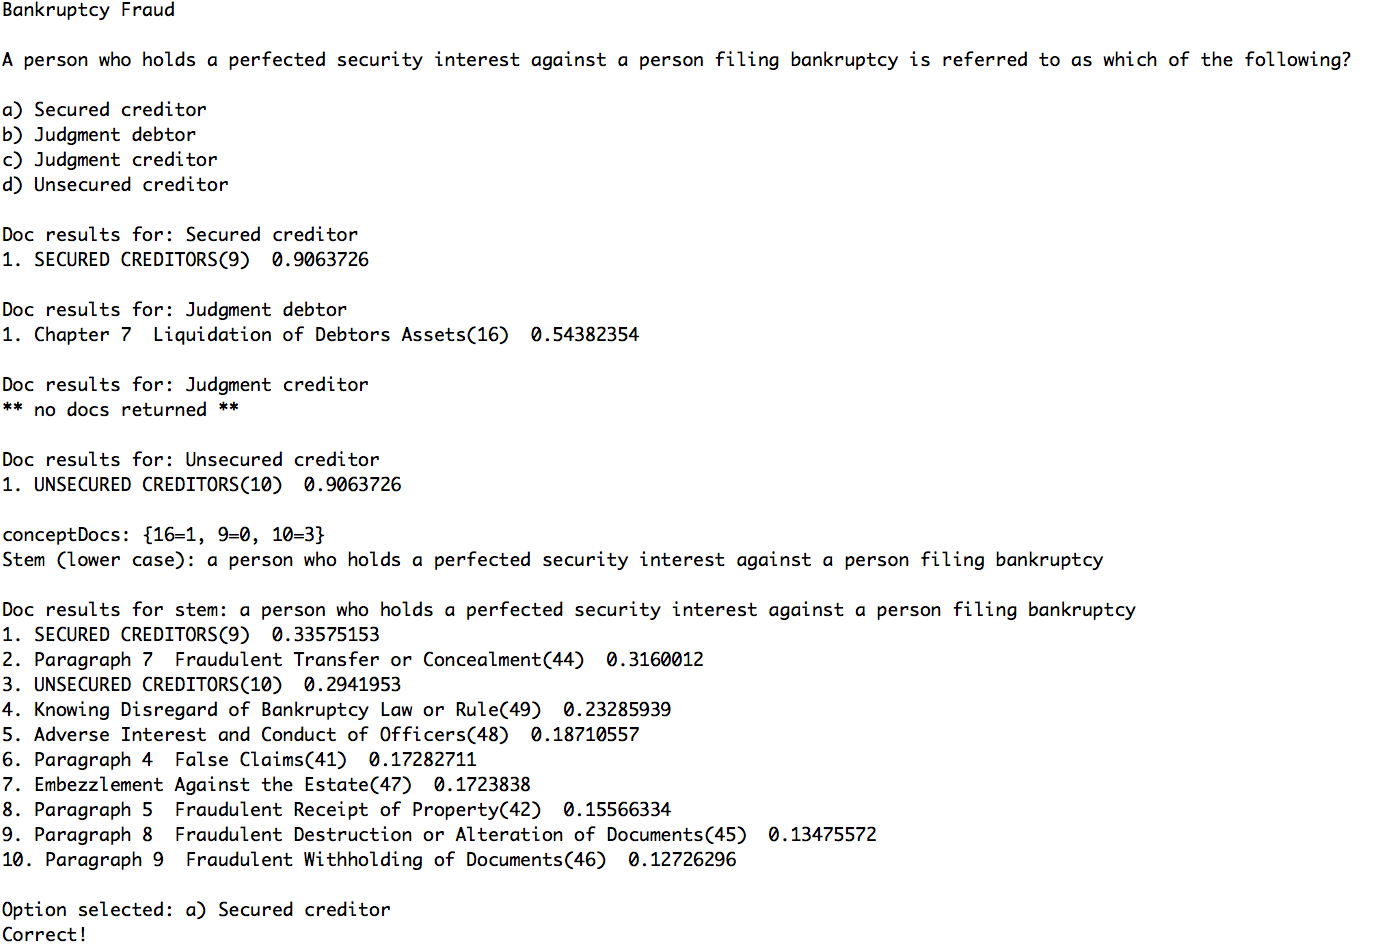
\includegraphics[width=125mm, height=125mm]{concept_match_v1_example.png}
\caption{Concept Match V1 Example}
\label{fig:concept_match_v1_example}
\end{figure}


\subsubsection{Agent Justification for Selected Answer}

Notice, in the above example, that the agent shows its reasoning for its argument.  By giving the scored return set for the question stem, and for each option, the agent provides the detail for its argument for the option it selects.  It is clear from the detailed output that among the documents in the returns set for the question stem query and among the set of documents in the return sets for the question options queries, there are two documents that appear in both - SECURED CREDITORS, (id = 9) and UNSECURED CREDITORS (id = 10).  Since the SECURED CREDITORS document earns a higher vectorization match score of 0.3375, the reasoning for selecting the Secured creditors, option a, is clear.

\subsubsection{Concept Match V1 Performance}

Finally, we look at the performance of the Concept Match Version 1 algorithm.  Fig.~\ref{fig:concept_match_v1_training_set_results_def} shows output from the algorithm tester tool described above, showing that among the 150 questions in the training set that were classified as strictly definition questions, (there were others that met the criterion for a definition question, but were classified in different but related categories, such as in the definition/not category, or definition/except category), this algorithm correctly answered 56 questions, or 37.3\% -- not an outstanding rate.  In fact it is lower than the rate of the Version 1 agent on these questions (41.3\%) using the maximum frequency algorithm based on the much shallower breakdown of the CFE manual into question sections.  However, these results also show that for 46 questions this algorithm produced no answer at all.  This was because the laser-focused question option queries against the title field of the documents in some cases returned 0 documents for \emph{all} options, thereby causing the algorithm to fail.  Fig.~\ref{fig:concept_match_v1_financial_statement_fraud_9} shows an example of this scenario.  With no documents in the set of return sets for the option queries, the algorithm has no other choice than to return -1, (for no option selected).  In the next algorithm, Concept Match V2, however, this issue is addressed.


\begin{figure}
\centering
\vspace{1.0in}
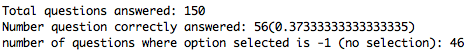
\includegraphics[width=75mm, height=15mm]{concept_match_v1_training_set_results_def.png}
\caption{Performance of Concept Match V1 on Definition Questions}
\label{fig:concept_match_v1_training_set_results_def}
\end{figure}

\begin{figure}
\centering
\vspace{1.0in}
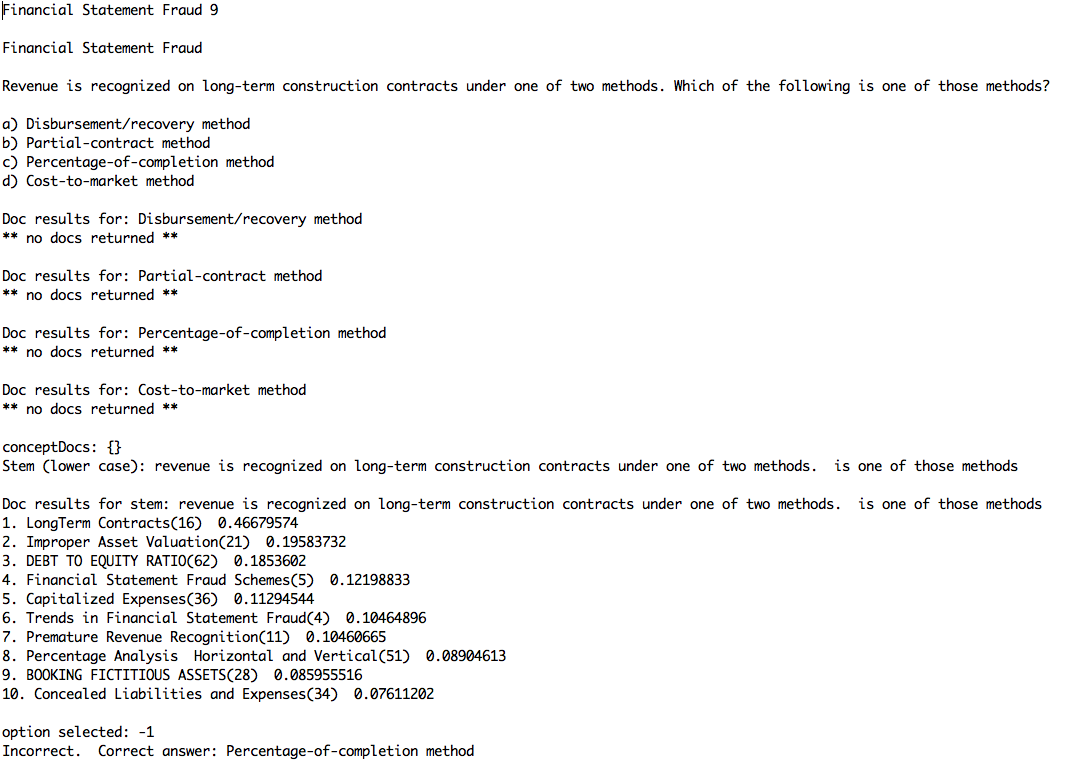
\includegraphics[width=125mm, height=125mm]{concept_match_v1_financial_statement_fraud_9.png}
\caption{Concept Match V1: An Example Where No Docs Are Returned for Options}
\label{fig:concept_match_v1_financial_statement_fraud_9}
\end{figure}


\subsection{Concept Match Version 2}

Concept Match Version 2 extends Concept Match V1 by addressing two major concerns.  The first is the situation outlined above in which for the query options no documents are returned because of the tight focus of the queries on the title field.  In Concept Match V2, if this scenario occurs, the options docs set is rebuilt, but instead of searching on the title field, the the search is performed on the contents field, thus, loosening the focus of the query resulting in a greater likelihood of documents in the return set that also occur in the question stem return set.  

The two figures, Fig.~\ref{fig:concept_match_v2_financial_statement_fraud_9_1} and Fig.~\ref{fig:concept_match_v2_financial_statement_fraud_9_2}  show the output for Concept Match V2 for the same example as  Fig.~\ref{fig:concept_match_v1_financial_statement_fraud_9} shows for Concept Match V1.  Again, this output shows the failure to return any documents or the option queries against the title field.  But whereas the V1 algorithm gives up and returns -1, V2 redoubles its efforts by re-issuing the same option queries against the contents field.  We see that in this example this form of recourse results in the algorithm producing the correct answer.

\begin{figure}
\centering
\vspace{1.0in}
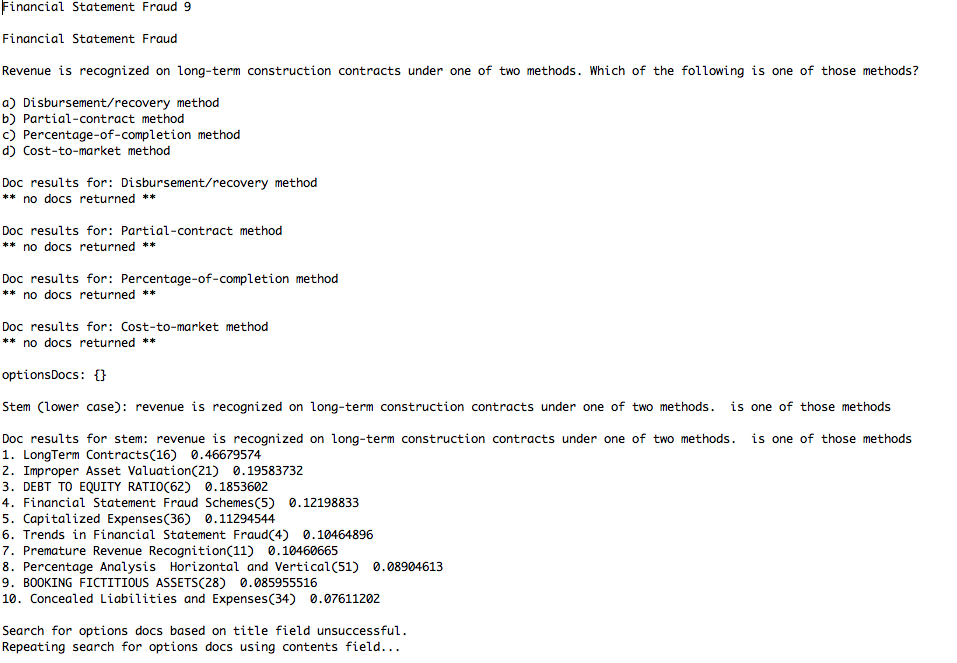
\includegraphics[width=125mm, height=125mm]{concept_match_v2_financial_statement_fraud_9_1.png}
\caption{Concept Match V2: Fixing the No Docs in Option Queries Return Sets Problem, Part 1}
\label{fig:concept_match_v2_financial_statement_fraud_9_1}
\end{figure}

\begin{figure}
\centering
\vspace{1.0in}
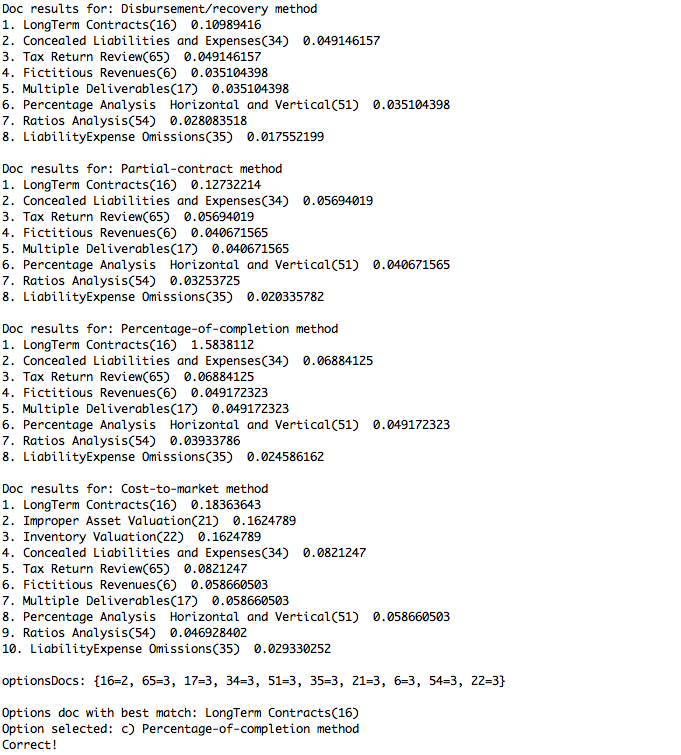
\includegraphics[width=125mm, height=125mm]{concept_match_v2_financial_statement_fraud_9_2.png}
\caption{Concept Match V2: Fixing the No Docs in Option Queries Return Sets Problem, Part 2}
\label{fig:concept_match_v2_financial_statement_fraud_9_2}
\end{figure}

The second major concern this this algorithm addresses is demonstrated by the following example shown in Fig.~\ref{fig:concept_match_v1_wrong_option_doc}.  In this case, we have a question in which the highest scoring document, (and by the way, the document which does, in fact, contain the answer to this question), ``The Business Profile Analysis", (id = 38), in the question stem return set is returned for \emph{two} options - option b, Preparing the business profile, and option c,  Preparing the vertical analysis.  Because Concept Match V1 simply loads these documents into the concept documents hash map in order by option, document 38 is \emph{initially} mapped to option b (the correct answer).  But then, this mapping is overwritten with a mapping to option c.  We can see this association in the display of the contents of the concept docs hash map, (the line in the output that starts with ``conceptDocs:"), in which we see the key/value association, 38=2, signifying that document 38 is associated with option 2 (i.e., option c; note that the option ids are 0-based, so option a is 0, option b is 1, option c is 2, and option d is 3).  As a result, the agent gets this question wrong.

\begin{figure}
\centering
\vspace{1.0in}
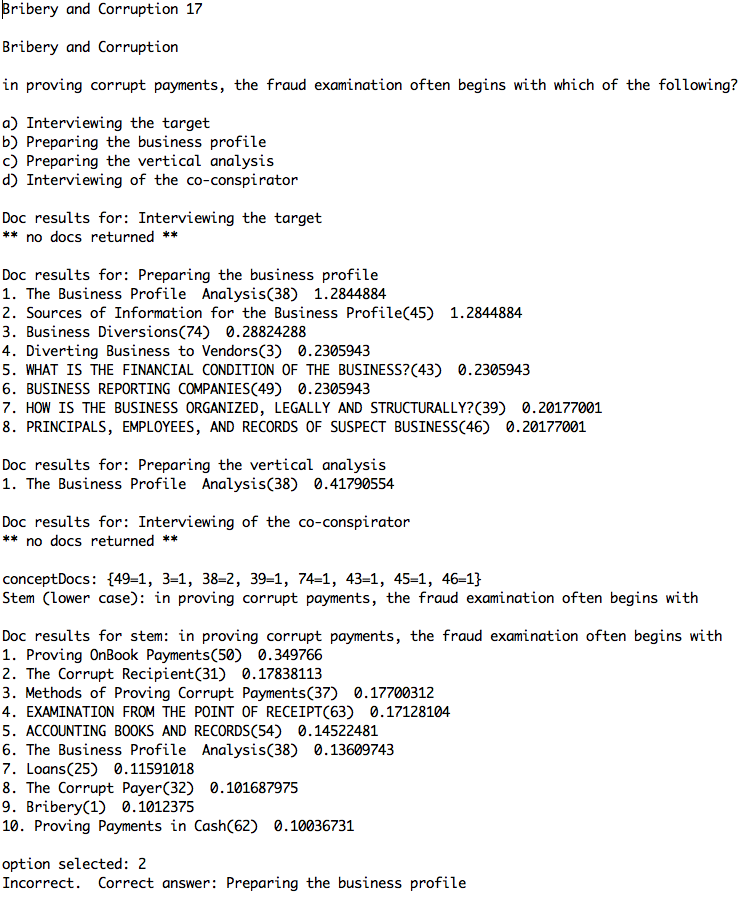
\includegraphics[width=125mm, height=125mm]{concept_match_v1_wrong_option_doc.png}
\caption{Concept Match V1: An Example Where A Document is Returned/Ranked for More than One Option}
\label{fig:concept_match_v1_wrong_option_doc}
\end{figure}

Concept Match Version 2 corrects this problem by recognizing a situation in which a document is included in multiple question-option-return-sets.  In this case, the algorithm maps the document to the option for which that document earned the highest rank score.  (Note that the lucene scoring algorithm is normalized so that scores for documents from different queries may be compared.)  Explaining this a bit more rigorously, for each concept document, $D$, with score, $S$, with respect to option $O$, if there is already an entry in the hash table for which the there is key/value pair, $D=(O',S')$, where $O'$ is a different question option and $S'$ is the score for $D$ with respect to $O'$, then scores, $S$ and $S'$ are compared, and the option whose score is maximum is chosen. If $S' > S$, then the entry with $D = (O',S')$ is left as is in the hash map. On the other hand, if $S' < S$, then the entry is overwritten with $D = (O,S)$.

For the ``Bribery and Corruption" example discussed below, we see in Fig.~\ref{fig:concept_match_v2_multiple_concept_docs} that Concept Match V2 properly associates the document, ``The Business Profile Analysis" (id = 38), with the correct option, ``b) Preparing the business profile".  The printout of the conceptDocs hash map shows the correct key/value association, 38=1, signifying that document 38 is now associated with option b, as opposed to option c.


\begin{figure}
\centering
\vspace{1.0in}
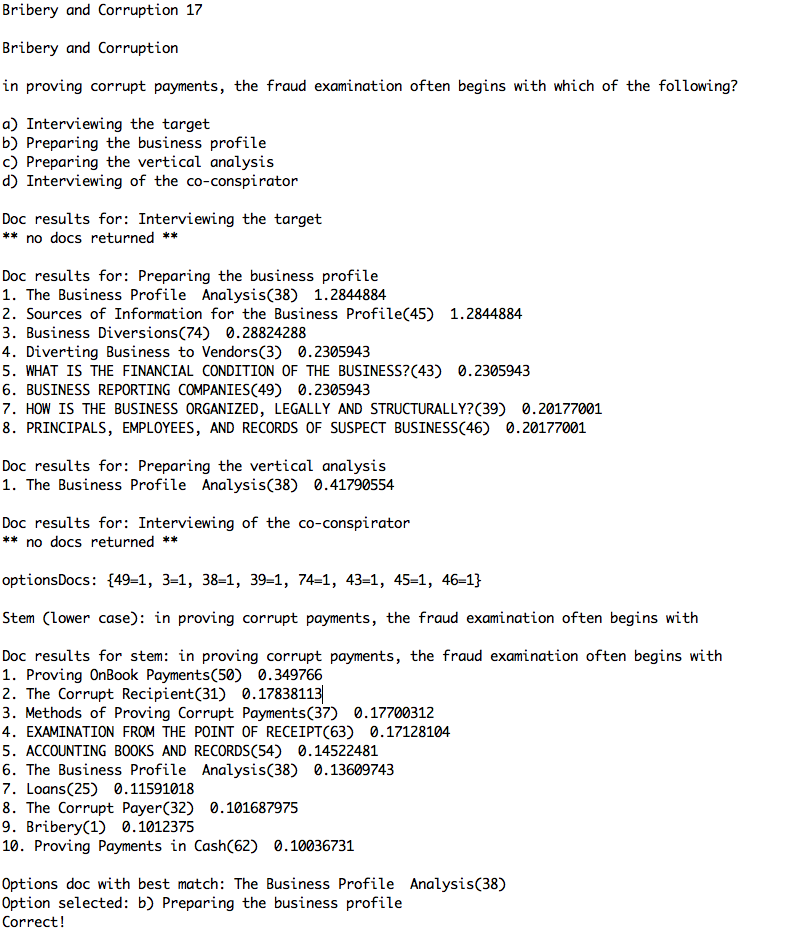
\includegraphics[width=125mm, height=125mm]{concept_match_v2_multiple_concept_docs.png}
\caption{Concept Match V2: Addressing the Problem of Multiple Options for a Document}
\label{fig:concept_match_v2_multiple_concept_docs}
\end{figure}

\subsubsection{Concept Match V2 Performance}

Next, we look at the performance of the Concept Match Version 2 algorithm on the same collection of questions which fall into the strictly defined definition-question category that were used to test Concept Match V1.  Fig.~\ref{fig:concept_match_v2_training_set_results_def} shows output from the algorithm tester shows this algorithm correctly answered 101 questions out of the collection of 150 definition questions, or 67.3\%, indicating a dramatic improvement in performance over that for Concept Match V1.  We also see that this algorithm has a much lower population of unanswered questions, (3 instead of 46), as a result of the fallback query measure incorporated into V2.



\begin{figure}
\centering
\vspace{1.0in}
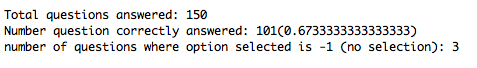
\includegraphics[width=75mm, height=15mm]{concept_match_v2_training_set_results_def.png}
\caption{Performance of Concept Match V2 on Definition Questions}
\label{fig:concept_match_v2_training_set_results_def}
\end{figure}

Fig.~\ref{fig:concept_match_v2_hypothesis_test} shows the results of a hypothesis test determining whether we can conclude a statistically significant improvement in accuracy as a result of the Concept Match V2 algorithm over that employed by Version 1 of the CFE agent, the Max Frequency algorithm, whose accuracy rate is 48.0\%.  This analysis shows that we can, in fact, draw the conclusion that Concept Match V2 offers a statistically significant improvement in performance at the 99\% confidence level.

\begin{figure}
\centering
\vspace{1.0in}
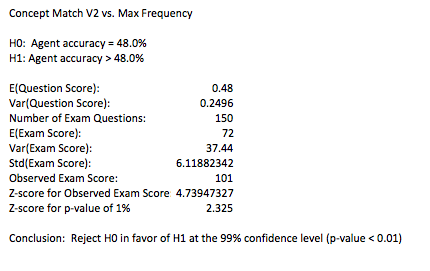
\includegraphics[width=75mm, height=60mm]{concept_match_v2_hypothesis_test.png}
\caption{Concept Match V2 vs. Max Frequency Hypothesis Test on Definition Questions}
\label{fig:concept_match_v2_hypothesis_test}
\end{figure}


\subsection{Concept Match Version 3}

Concept Match V3 attempts to build on Concept Match V2 by leveraging a behavior that was noticed in the results of the Lucene search results of the stem query.  
During development, it was noticed in a plurality of cases that  return sets for the question-stem query were headlined by a document whose score was head-and-shoulders above the rest of the docs in the return set, sometimes by a factor of three or more.  In these cases, it was commonly the case that this first-place document was, in fact, the correct document which contained the answer to the question.  So, when we have a document that hereafter will be referred to as a  ``premier document", the algorithm should focus on finding the option most closely associated with that premier document.  Concept Match V3 implements this approach by conducting queries for the options and choosing the option for which the premier document scores highest.  If no query-option queries based on the title field yield the premier document, then the algorithm repeats the query-option queries against the contents field of the document collection.  If the premier document \emph{still} does not appear in any result set, the algorithm returns -1, representing no selection.

Consider the example in Fig.~\ref{fig:concept_match_v3_example_part_1} and Fig.~\ref{fig:concept_match_v3_example_part_2}.  The question stem query for this ``Criminal Prosecutions for Fraud" question returns a result set in which the ``Arraignment" document, (id=12), with a score of 0.4654 outscores the next place document, ``Sentencing" (id=45) by a facor of more then 2.5x.  The algorithm, therefore,  categorizes this document as a premier document, and thus approaches the option selection process by attempting to find the option whose query result ranks this document higher than that for any other option.  In this example, we see that for the option queries based on the title field, the result sets are thin and there's no match to the premier document.  In this case, the algorithm re-issues the option queries, but this time casts a wider net by going aginst the contents field of each document in the collection.  In Fig.~\ref{fig:concept_match_v3_example_part_2}, we see that this approach prevails -- the result set for the correct answer, option b, the Alford plea, includes the Arraignment document.  Further, we see that although this document appears in the result sets for other options' queries, it scores highest for the Alford plea option.

\begin{figure}
\centering
\vspace{0.75in}
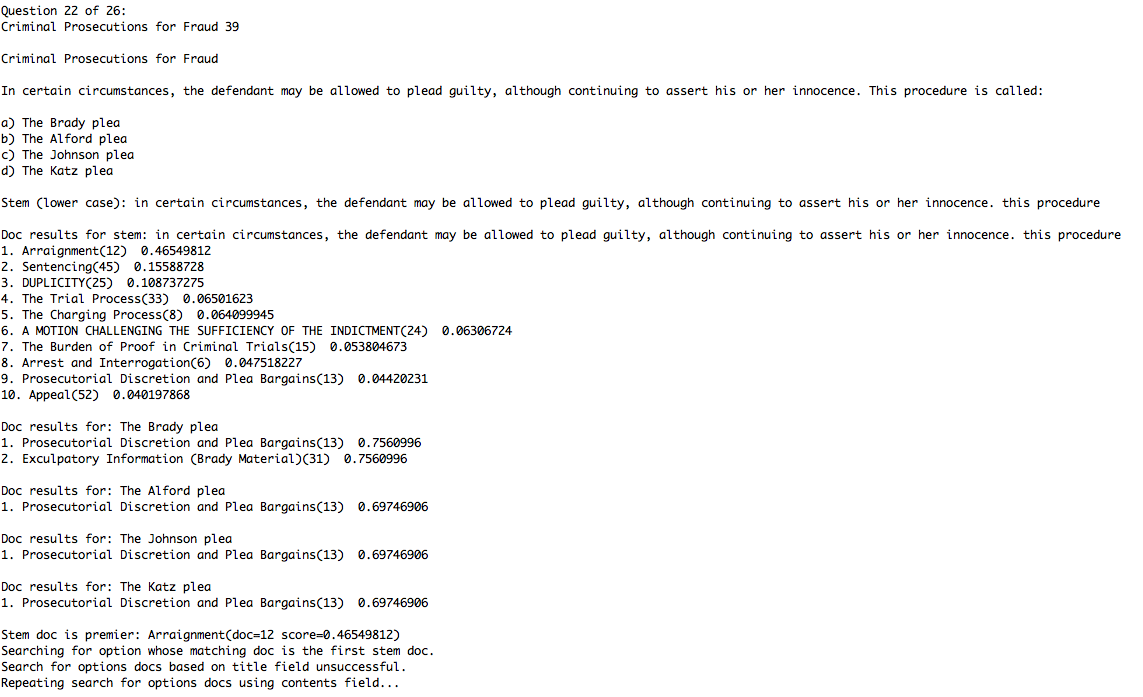
\includegraphics[width=125mm, height=125mm]{concept_match_v3_example_part_1.png}
\caption{Concept Match V3 Example - Part 1}
\label{fig:concept_match_v3_example_part_1}
\end{figure}

\begin{figure}
\centering
\vspace{0.75in}
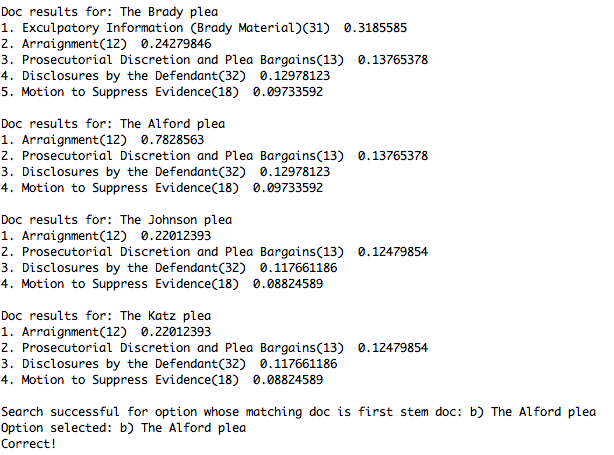
\includegraphics[width=125mm, height=125mm]{concept_match_v3_example_part_2.png}
\caption{Concept Match V3 Example - Part 2}
\label{fig:concept_match_v3_example_part_2}
\end{figure}

Fig.~\ref{fig:concept_match_v3_example_document} shows the ``Arraignment" document.  It provides a couple of key insights as to the behavior of the algorithm on this particular question.  First, we notice that the answer to the question is provided on lines 39 through 42.  The brief segment shown here concerning a description of the Alford plea suggests (and, in fact, it turns out to be the case upon further checking) that there is no document in the collection specifically dedicated to (and whose title field would be) the Alford plea.  Second, a cursory examination of this document reveals that there are number of occurrences of the term, ``plea" throughout the document which would explain why this document appears in the result set for not only the Alford plea option, but also for the Brady plea, Johnson plea, and Katz plea options.  However, the name, ``Alford" is the only one of these names mentioned in this document, and this explains why for the Alford plea option, this document scores significantly higher than for any other option.

\begin{figure}
\centering
\vspace{0.75in}
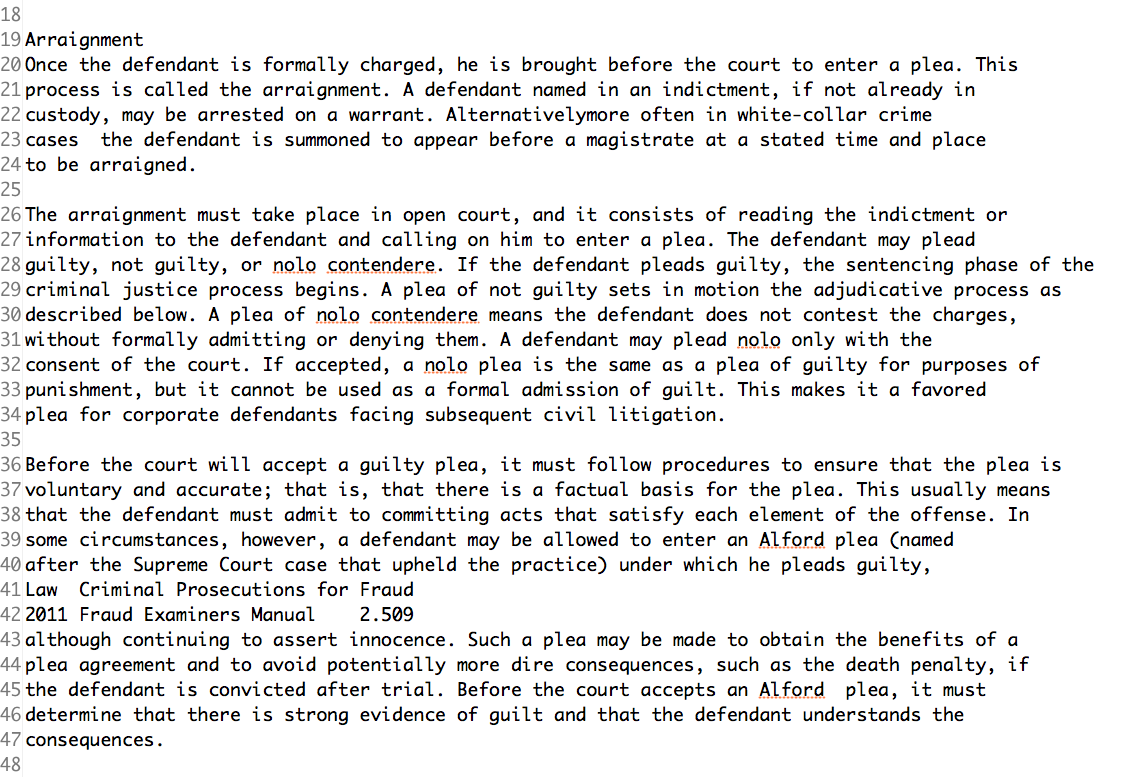
\includegraphics[width=125mm, height=125mm]{concept_match_v3_example_document.png}
\caption{The Arraignment Document}
\label{fig:concept_match_v3_example_document}
\end{figure}


\subsection{Concept Match V3 Performance}

Fig.~\ref{fig:concept_match_v3_training_set_performance} shows the performance of the Concept Match V3 algorithm on the 150 definition-type questions of the training set.  It shows that V3 improves on V2 slightly, getting 105 question correct compared with V2's 101.  However, this improvement is not significant enough to be statistically significant at the 99\% level, as the figure~\ref{fig:concept_match_v3_hypothesis_test} shows.  Nonetheless, the fact that V3 outpaces V2 means that the CFE agent will use V3 over V2 when confronted with a definition-type question, (and, as we'll see later, the agent will use this algorithm on other types of questions as well).  And finally, lest we forget, compared with Version 1 of the agent, this algorithm extends the gains we achieved with Concept Match V2 that were, themselves, found to be statistically significant relative to Version 1 of the CFE agent.

\begin{figure}
\centering
\vspace{0.75in}
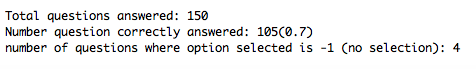
\includegraphics[width=75mm, height=15mm]{concept_match_v3_training_set_performance.png}
\caption{Performance of Concept Match V3 on Training Set}
\label{fig:concept_match_v3_training_set_performance}
\end{figure}



\begin{figure}
\centering
\vspace{0.75in}
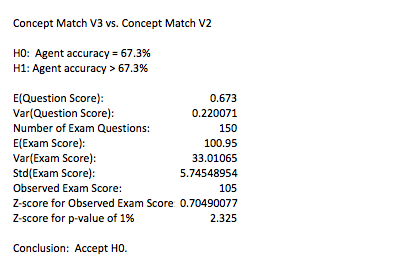
\includegraphics[width=75mm, height=60mm]{concept_match_v3_hypothesis_test.png}
\caption{Concept Match V3 vs. V2 Hypothesis Test on Definition Questions}
\label{fig:concept_match_v3_hypothesis_test}
\end{figure}



\subsection{Concept Match NOT}

Concept Match NOT extends the logic of Concept Match V3, but turns it on its head to handle questions of the type, ``Which of the following is NOT ...'', where for the phrase that follows, all options are true except for one, and of course, the agent must choose that option to correctly respond to the question.  An example of a question of this type is ``Which of the following is NOT a plea a defendant may enter at an arraignment?"
Concept Match NOT takes an approach that inverts the over-arching approach of the algorithms we've discussed above.  Instead of looking for the option for which there's the greatest affinity between option query result sets and the question stem result set, Concept Match NOT find the option whose result set has the least affinity.  

Fig.~\ref{fig:concept_match_not_example_part_1} and Fig.~\ref{fig:concept_match_not_example_part_2} show an example of this algorithm at work.  First, as we saw in the agent's justification in earlier algorithms, we see the result set for the question stem query, and then those for the option queries.  The agent then sets about attempting to map the overlap between the question stem result set and the option result sets by building two hash maps.  The first one, the ``docOptionScores" map, associates each document among the option query result sets with the the option for which that document earned the highest score.  The algorithm then utilizes this data to construct the second hash map, ``optionScoreDocs", which consists of option/document key/value pairs for which the documents are present in both the ``docOptionScores" map and in the question stem result set.  Using this data structure, the agent makes a selection; specifically, it selects the option whose document has the weakest affinity with the question stem result set.  In this case, that's option d, skimming, since this option has no representation in the optionScoreDocs data structure, implying it has no documents that overlap with the result set of the question stem.  (Looking closely, we see that whereas all of the other option queries have result sets that are non-empty, the the result set for the skimming option has no documents, and so, it's reasonable that it has the weakest affinity with the question stem.) 



\begin{figure}
\centering
\vspace{0.75in}
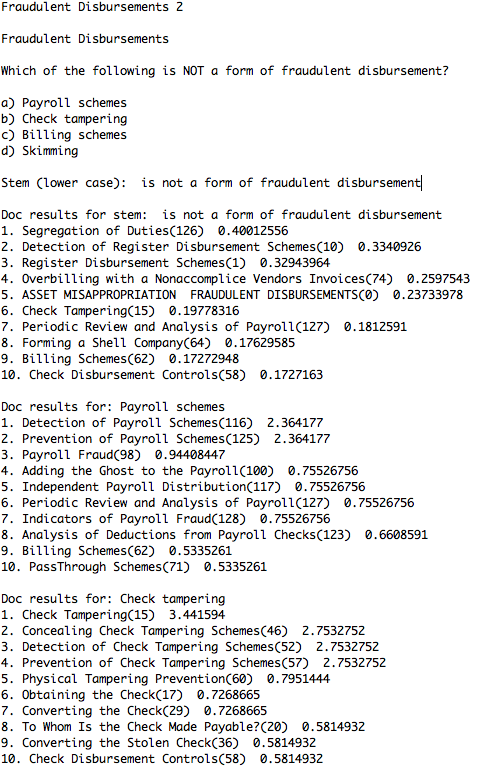
\includegraphics[width=125mm, height=125mm]{concept_match_not_example_part_1.png}
\caption{Concept Match Not Example - Part 1}
\label{fig:concept_match_not_example_part_1}
\end{figure}

\begin{figure}
\centering
\vspace{0.75in}
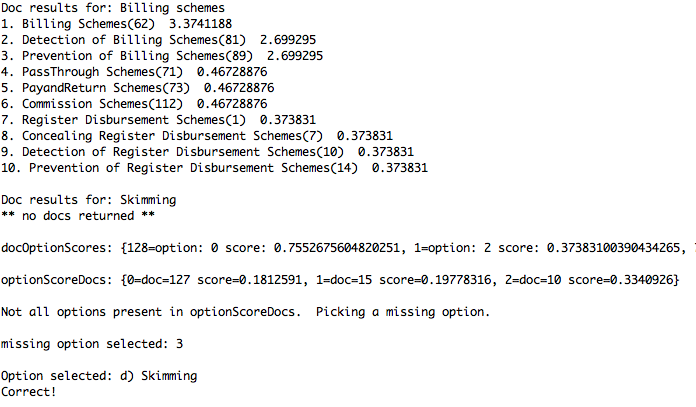
\includegraphics[width=125mm, height=90mm]{concept_match_not_example_part_2.png}
\caption{Concept Match Not Example - Part 2}
\label{fig:concept_match_not_example_part_2}
\end{figure}

\subsection{Performance of the Concept Match NOT on the Training Set - Definition/NOT Questions}

Fig.~\ref{fig:concept_match_not_training_set_performance} shows the performance of the Concept Match NOT algorithm on Definition/NOT questions in the training set - 8 out of 27 correct, or 29.6\%.  It is not unreasonable to expect that this algorithm would show weaker performance than its inverted cousin, Concept Match V3, as discovering the negative, as we are attempting to do in the case for this question type, is difficult to do.  In fact, we cannot reject the null hypothesis that this algorithm performs any better on Definition/NOT questions than random guessing, as shown in Fig.~\ref{fig:concept_match_not_hypothesis_test}.  Further investigation is required to refine this algorithm or to take a different approach with these types of questions altogether.


%However, even with that disadvantage, the Concept Match Not algorithm shows statistically significant improvement over random approach at the 99\% confidence level.  Note, we compare this algorithm to random selection because in Version 1 of the CFE Agent we observe that no algorithm actually did any better than random selection for this type of question, refer to Fig.~\ref{fig:version_1_training_set_results_not}.

\begin{figure}
\centering
\vspace{0.75in}
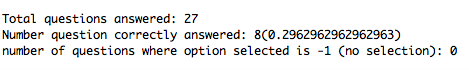
\includegraphics[width=75mm, height=13mm]{concept_match_not_training_set_performance.png}
\caption{Performance of Concept Match Not on Training Set - Definition/NOT Questions}
\label{fig:concept_match_not_training_set_performance}
\end{figure}

\begin{figure}
\centering
\vspace{0.75in}
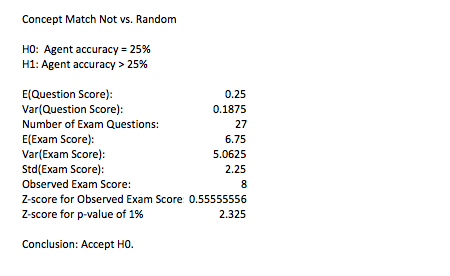
\includegraphics[width=75mm, height=60mm]{concept_match_not_hypothesis_test.png}
\caption{Concept Match Not vs. Random Hypothesis Test on Definition/Not Questions}
\label{fig:concept_match_not_hypothesis_test}
\end{figure}




\subsection{Concept Match NOTA}

Concept Match NOTA leverages the logic in Concept Match V3 for concept matching, and extends it for addressing definition questions in which the last option is ``none of the above''.  Hereafter, we'll refer to such questions as NOTA questions.

The first concern to investigate in developing this algorithm was the frequency with which the ``none of the above" option was actually the correct response in NOTA questions.  In order to determine this, we developed a trivial algorithm, called the None Of the Above Algorithm, which simply selects the last option, that is, the ``none of the above" option, always.  Then, we ran this algorithm on all 162 NOTA questions in the training set.  The ratio of the correctly answered questions for this algorithm gave us our answer.  Fig.~\ref{fig:nota_training_set_performance} shows the performance results.  We see that the ``none of the above" option is under-represented as a correct answer, serving as the correct answer only 7.4\% of the time.  Whereas we'd expect that it should be the correct answer 25\% of the time, it is, in fact, drastically under-represented as the correct answer.  This served as the inspiration for the simplistic but strategic approach of this algorithm - simply remove the ``none of the above option" as one of the possible options and select from the remaining three options (using the logic of Concept Match V3).

\begin{figure}
\centering
\vspace{0.75in}
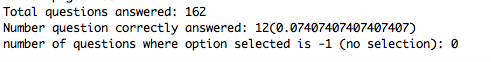
\includegraphics[width=75mm, height=13mm]{nota_training_set_performance.png}
\caption{Performance of NOTA Algorithm on NOTA Questions}
\label{fig:nota_training_set_performance}
\end{figure}


Fig.~\ref{fig:concept_match_nota_example} shows an example of the execution of this algorithm.  The agent collects the result set for the question stem query, notices that this question is a NOTA question and thus, removes the ``none of the above" option from its set of options, infers from the score of the ``Quiet Rooms" document (id=171) relative to that of the second place document that its a premier document, and picks the option for whose query scores the ``Quiet Rooms" document higher than any other option.  This leads to the correct selection of a) Quiet Rooms.


\begin{figure}
\centering
\vspace{0.75in}
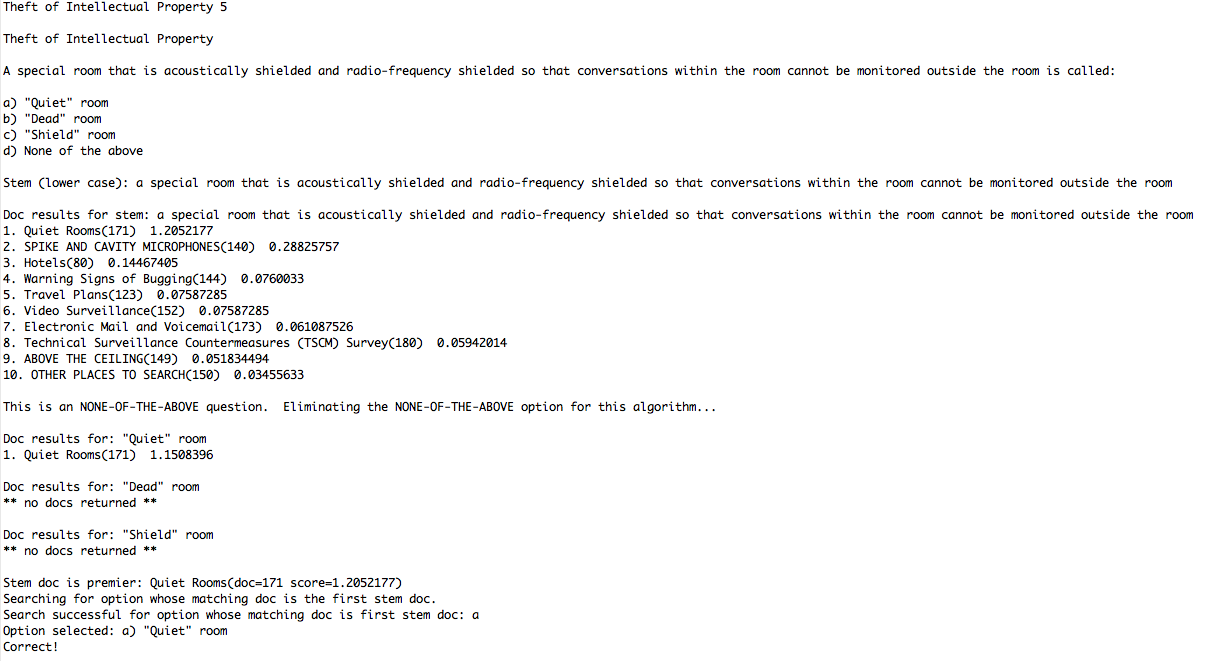
\includegraphics[width=125mm, height=100mm]{concept_match_nota_example.png}
\caption{Concept Match NOTA Example}
\label{fig:concept_match_nota_example}
\end{figure}

\subsection{Performance of Concept Match NOTA}

Fig.~\ref{fig:concept_match_nota_training_set_performance} shows the performance of this algorithm on the Definition/NOTA questions at 65.4\% accuracy.  Fig.~\ref{fig:concept_match_nota_hypothesis_test} shows a hypothesis test of this algorithm against the Max Frequency algorithm which had the best results in the CFE Agent Version 1.  Since Max Frequency showed results of 56.5\% on 162 questions, the results of Concept Match NOTA were \emph{just short} of showing statistically significant improvement at the 99\% confidence level.  However, notice that the improvement posted by this algorithm \emph{is} significant at the 98\% confidence level.  Given this, we incorporate this algorithm into the agent as part of its enhanced suite of tools of Version 2.

\begin{figure}
\centering
\vspace{0.75in}
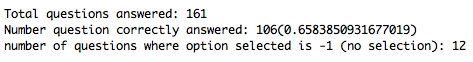
\includegraphics[width=75mm, height=13mm]{concept_match_nota_training_set_performance.png}
\caption{Performance of Concept Match NOTA on Training Set - Definition/NOTA Questions}
\label{fig:concept_match_nota_training_set_performance}
\end{figure}



\begin{figure}
\centering
\vspace{0.75in}
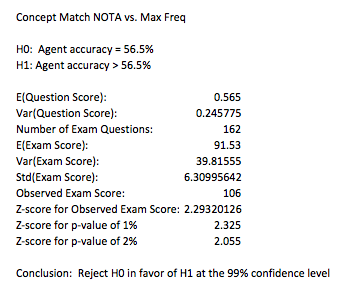
\includegraphics[width=100mm, height=75mm]{concept_match_nota_hypothesis_test.png}
\caption{Concept Match NOTA vs. Max Frequency Hypothesis Test on Definition/NOTA  Questions}
\label{fig:concept_match_nota_hypothesis_test}
\end{figure}





\section{CFE Agent Version 2 Results}

Fig.~\ref{fig:version_2_training_set_performance} summarizes the performance of the CFE Agent Version 2.  It shows that with a 70.0\% accuracy rate on definition questions, Concept Match V3 is the preferred algorithm for that question type.  And Concept Match NOT is the preferred algorithm for definition/NOT questions, even with the disappointing accuracy rate of only  29.6\%.  This algorithm also emerges as the favorite for definition/EXCEPT questions (``All of the following are .... EXCEPT ....") as well, with an accuracy rate of 46.7\%.  This is not surprising as this type of question is semantically equivalent to the Definition/NOT question, so it is reasonable for this algorithm to be the top performer for this type as well.  Finally, Concept Match NOTA is the preferred algorithm for NOTA questions, with an accuracy of 65.8\%.

%\begin{figure}
%\centering
%\vspace{0.75in}
%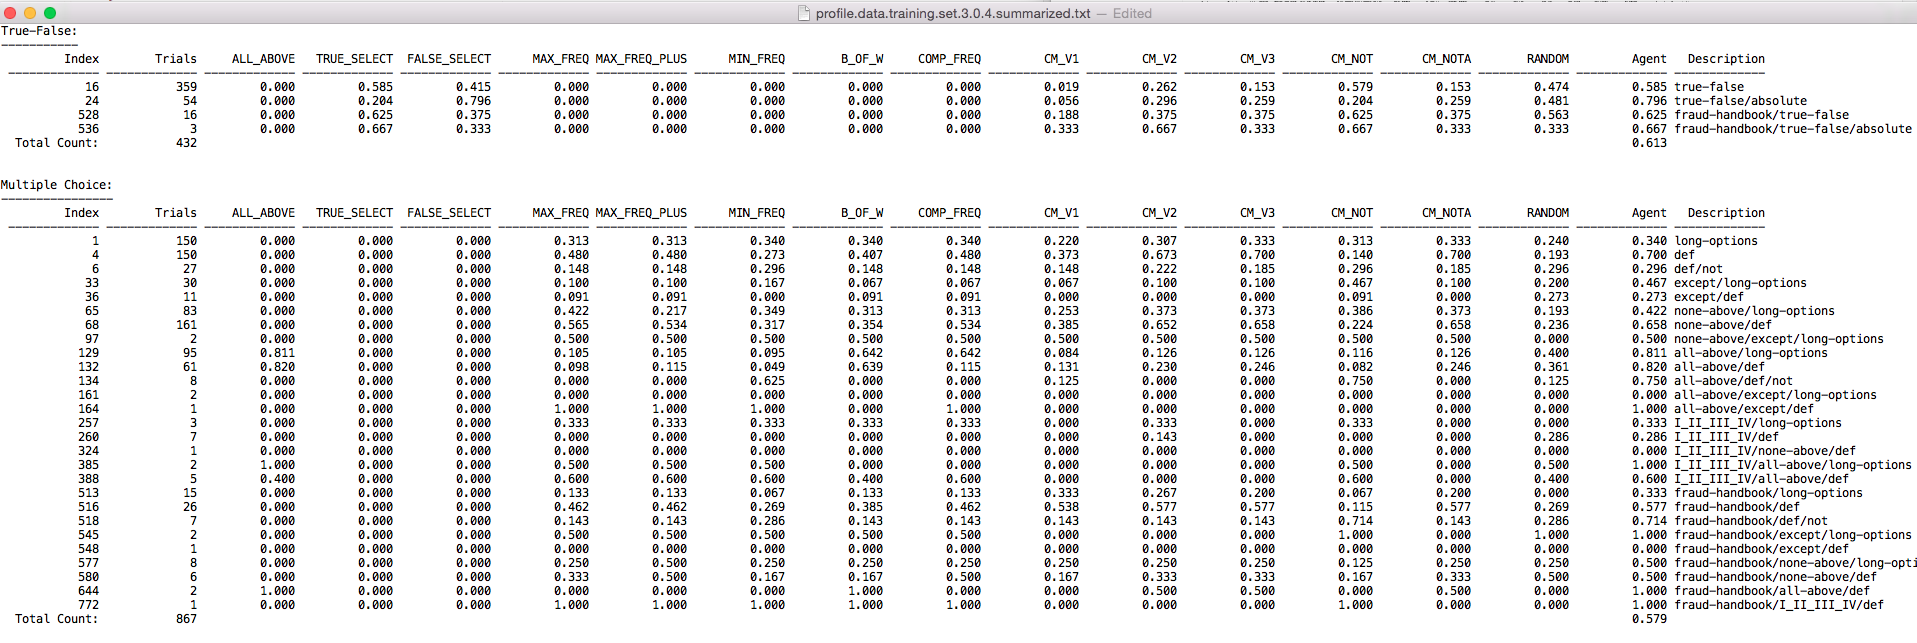
\includegraphics[width=125mm, height=100mm, angle=90]{version_2_training_set_performance.png}
%\caption{Performance of CFE Agent Version 2 on Training Set}
%\label{fig:version_2_training_set_performance}
%\end{figure}

\begin{sidewaysfigure}
\centering
\vspace{0.25in}
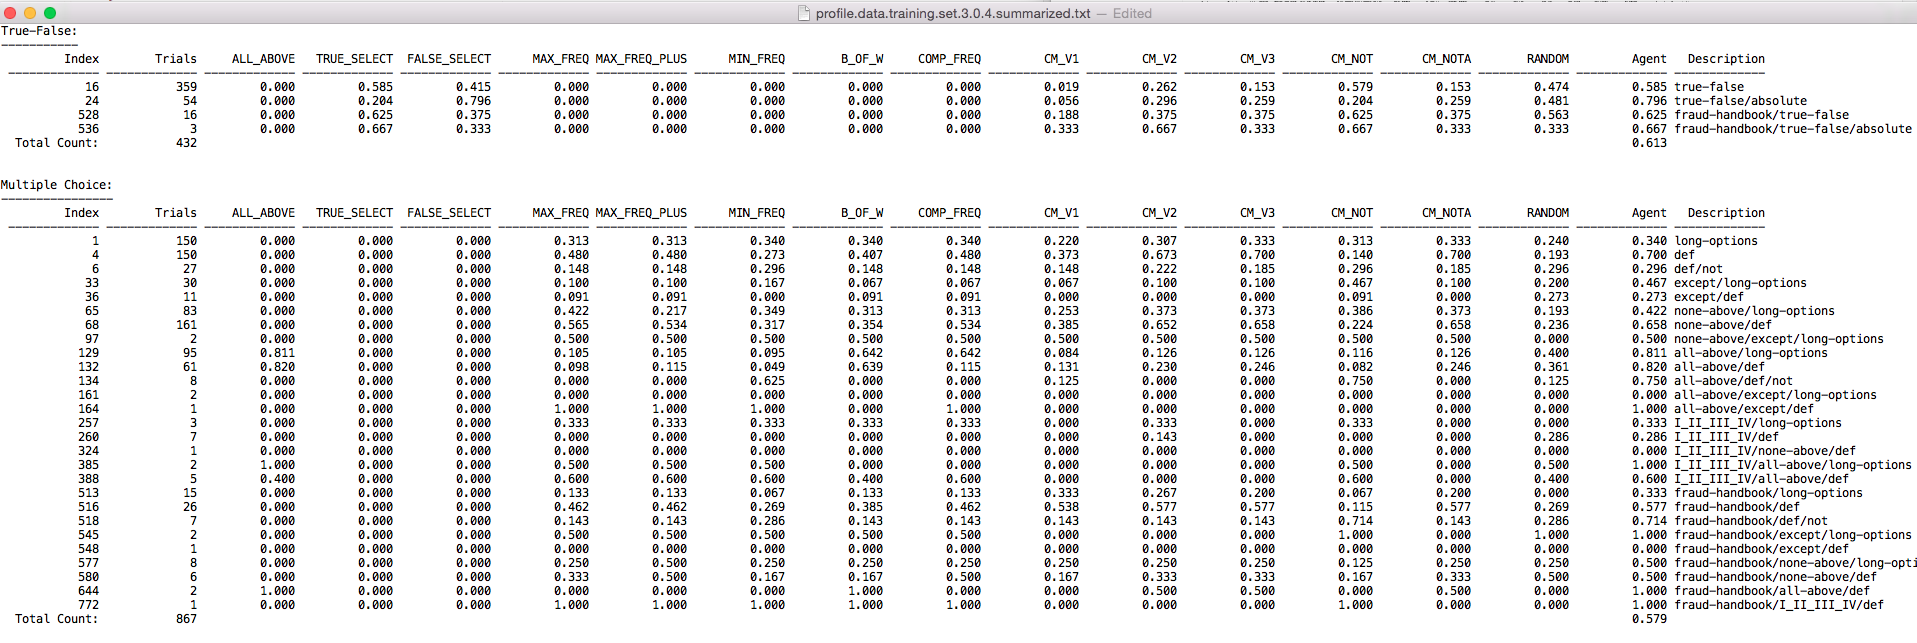
\includegraphics[width=\textwidth]{version_2_training_set_performance.png}
\caption{Performance of CFE Agent Version 2 on Training Set}
\label{fig:version_2_training_set_performance}
\end{sidewaysfigure}

Fig.~\ref{fig:version_2_multiple_choice_hypothesis_test} shows the results of a hypothesis test of the performance of the CFE Agent Version 2 on the entire battery of training set questions relative to that of Version 1.  The analysis shows the improvement for Version 2 over Version 1 to be statistically significant at the 99\% level.  This should not be surprising since the question types for which we've targeted our new algorithms, namely Definition, Definition/NOT, and Definition/NOTA , constitute a large portion of the question battery (338 of the 867 questions), as indicated by the Trials column of the table in Fig.~\ref{fig:version_2_training_set_performance}.

\begin{figure}
\centering
\vspace{0.75in}
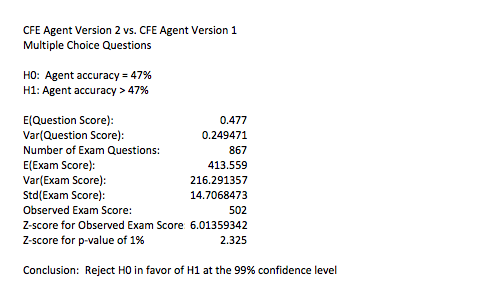
\includegraphics[width=75mm, height=60mm]{version_2_multiple_choice_hypothesis_test.png}
\caption{CFE Agent Version 2 vs. CFE Agent Version 1 Hypothesis Test on Multiple Choice Questions}
\label{fig:version_2_multiple_choice_hypothesis_test}
\end{figure}

Running the CFE Agent on the test set of 200 questions yields a score of 119 out of 200, or 59.5\%, a dramatic improvement over the 49\% of Version 1.

















 % chapter 4 - Intelligent Agent - Version 2
%%%%%%%%%%%%%%%%%%%%%%%%%%%%%%%%%%%%%%%%%%%%%%%%%%%%%%%%%%%%%%%%%%% 
%                                                                 %
%                            CHAPTER FIVE   - A Learning Agent - Version 3            %
%                                                                 %
%%%%%%%%%%%%%%%%%%%%%%%%%%%%%%%%%%%%%%%%%%%%%%%%%%%%%%%%%%%%%%%%%%% 
 
\chapter{Version 3 -- A Learning Agent}

In this chapter, we describe Version 3 of the CFE Agent and its development.  In Version 3, the agent attempts to isolate the passage from which each question is drawn at an even finer level of detail than in Version 2.  To review, Version 1 of the agent attempts to answer question using a very course-grained filter in which text is isolated only at the relatively high level of question section within the CFE Manual.  Version 2 attempts to improve on this by decomposing the large sections of the manual into documents according to table-of-contents entries and specific text features, such as, capitalized sub-headings.  In Version 3, the agent breaks up the text even further dividing each document into passages, and attempts to isolate the single passage most relevant to the question.  It should be noted, however, that Version 3 focuses exclusively on definition-type questions, unlike Versions 1 and 2, for which performance was analyzed and discussed on many or all question types in the preceding chapters in detail.  Given the narrow focus on a single passage for each question, it was thought that this approach is most appropriate for definition questions.  However, extending this approach to other question types is an area for further research.

The general approach for Version 3 is the application of supervised machine learning  \cite{alpaydin_2014_introduction_ch1}, in conjunction with information retrieval for selecting the ``most correct" passage for each question.  The machine learning model uses logisitic regression for discriminating a correct passage from an incorrect one, based on a prescribed set of features by assigning a probability of relevance to each passage.  After sorting these passages in descending order of probability, the agent selects a number of passages from the top of this list and uses a separate algorithm that selects an answer from among the four answer options.  By employing machine learning, however, we must concede that justifications for answers are more opaque, as it becomes more difficult to explain the coefficients that the agent uses in the logistic regression model.  Doing so would require a low level explanation connecting the questions and their passages in the training set to the learned coefficients of the model, which is not practical.  Thus the justifications for the agent's answers exclude this aspect of the algorithm.

%During development of Version 3, a number of considerations needed to be addressed, including the the decision of what should constitute a passage (a paragraph? a sentence? a phrase?), the features for the passage selection model, the selection of questions for the training set and test set, the manual curation of the training set and test set, the development of the model from the training set, and its application to the test set.  These issues are discussed in the sections below.  

This rest of this chapter is laid out as follows:  First, we discuss the preparation of the training and test sets, and in so doing explicitly describe how each of the issues mentioned above were handled, in detail.  Next, we describe the development of the logistic regression model for classifying passages as either relevant or irrelevant.  Third, we discuss the application of the model to the test set and discuss its performance.  And finally, we discuss two answer selection algorithms and their performance.

%\section{Machine Learning}

% describe machine learning in more detail here, much like we described information
% retrieval in chapter 04.

	%\subsection{Linear Regression}

	%\subsection{Logistic Regression}

\section{Development of the Training Set}

This section discusses the development of the training set for the passage classification model, describing in detail the questions selected for the training set and test set, and the up-front activities that were necessary to develop the model.


\subsection{Targeted Questions}

%As mentioned above, Version 3 of the agent is intended to further refine the text body upon which it answers each question.  As was the case in Version 2, the primary target for its algorithms are the definition questions.  Thus, the clear place to start for the training set was the pool of questions classified as definition questions.  Performance reports in Chapter 3 show that for the training set, there are 196 definition questions (profile 4).  

Given the the exclusive focus on definition questions, we included only the definition questions (profile 4 in Fig.~\ref{fig:version_2_training_set_performance}) in the training and test sets for Version 3. Fig.~\ref{fig:version_2_training_set_performance} indicates there are 150 such definition questions, (with a profile equal to 4), in the training set.  Furthermore, it was found that among these 150 questions, 133 of them had natural language explanations from which it was easy enough to programmatically extract the page number on which the relevant passage appeared for the question using regular expressions.  So, ultimately, the training set was whittled down to 133 definition questions.  Using the same approach, 16 definition questions were selected from among the 200 questions in the test set.  Certainly, it would have been desirable to have more questions in the test set, but it does reflect a selection percentage, 16 / 200 = 8\% that is roughly similar to the selection percentage from the training set, 133 / 1300 = 10\%.

\subsection{Passage Training Set}

Next, we set about the task of developing the training set of passages upon which the passage classification model is based.  The approach for accomplishing this can be described as follows:

\begin{enumerate}
\item Determine the proper unit for breaking up the documents into passages.  The choice here was to simply break up the passages along the lines of paragraphs.  The rationale for this was twofold.  First, paragraphs generally can be thought to contain a collection of units of meaning that make up a single larger unit, so there's a semantic rationale.  Second, the practical reason -- it's relatively simple to break up text by paragraph.

\item Determine the relevant passage for each question, manually.  This process, of course, required simply looking through the CFE Manual to find the right paragraph.  As mentioned above, using the page numbers programmatically extracted from the explanations for the questions was a huge help, here.  Still, this step constituted the most tedious part of the process.

\item Use Lucene to identify the relevant documents for each question.  This step utilized Lucene in the same way it was employed for Version 2.  That is, elements of the stem were isolated and used as the basis for the formation of a query which was then executed against the document collection for the applicable question section.  The 20 top-scoring documents were selected as the ones assumed to provide adequate coverage of the relevant passage.  That is, it was presumed likely that one of the top 20 documents contained the relevant passage determined in the last step.  The decision to use the number, 20, was arbitrary.  However, this number proved to be sufficient in all but 8 out of the 133 training set questions.  

\item Create the training set of passages.  This was accomplished by extracting each passage for each of the documents from the IR step, and correctly labeling it as relevant/irrelevant.  Note that for each question, the assumption was made that exactly one passage was relevant.  Again, as mentioned above, for all but 8 questions in the training set, there was one passage marked relevant.  All others were marked as irrelevant.  For the 133 definition questions of the training set, we generated 9419 passage records from the related documents.

\item Identify and determine the features for each passage.  There were a number of features used here as inputs to the logistic regression model.  Not surprisingly, we used the document search rank.  The higher the rank of the containing document, the more likely it would seem that the passage would be the relevant passage for the question.  Two other features were also used:  the number of distinct words in common between the question stem and the passage, and the length of the longest common sequence of words between the question stem and the passage.
\end{enumerate}

Note that the process of identifying the correct passage and of generating the passages was also applied to the test set.  For the 16 questions in the test set, we generated 971 passage records from the related documents.


\section{Development of the Passage Classification Model}

Fig~\ref{fig:logistic_model_summary} shows the output of the program written in R \cite{james_2013_introduction_ch4} for constructing the passage selection classification model.  As mentioned above, this model uses logistic regression to arrive at the constant coefficients shown in the figure.  Some clarification of the names of the input and output variables is needed here:  

\begin{enumerate}
\item dr -- (short for ``document rank") -- is an input variable containing Lucene's rank of the document containing the given passage using the question stem as the query string.
\item nwic -- (short for ``number words in common"") is an input variable containing the number of distinct words in common between the passage and the question stem
\item llcs -- (short for ``length longest common sequence") is an input variable giving the length of the longest sequence of words in common between the passage and the question stem.  
\item icp -- (short for ``is correct passage"), is the variable indicating whether the passage is the relevant passage, 1 if it is the correct passage, 0 otherwise.  All of the input variables show a significant relationship with the output variable as evidened by their respective z-scores, all of which indicate significance at the 99\% level of confidence.
\end{enumerate}

As for the coefficients, themselves, the coefficient for the document rank variable, has a negative sign.  This indicates, not surprisingly, a negative relationship with the output variable.  That is, the lower the value of document rank variable, (i.e., the closer it is to the value of 1), the higher the likelihood the passage is assigned the value 1, as opposed to 0.  The other two variables, nwic and llcs, both have positive coefficients, indicating a positive relationship with the output variables, as one would expect.

\begin{figure}
\centering
\vspace{1.0in}
\framebox{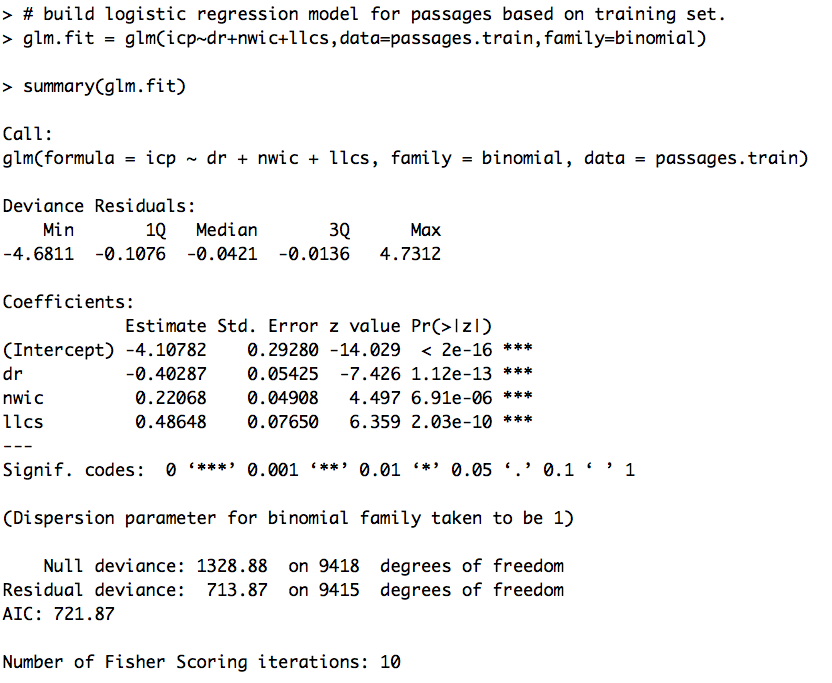
\includegraphics[width=125mm, height=125mm]{logit_model_summary.png}}
\caption{Passage Classification Model Summary}
\label{fig:logistic_model_summary}
\end{figure}


\section{Application to the Test Set}

The application of the classification model to the passage test set yields favorable results.  Fig.~\ref{fig:logit_model_test_set_top} shows an extract of the data, where each record corresponds to a passage (whose text is not shown).  The fields show the question id to which the passage applies, the input variables, including dr, nwic, and llcs, and the output variable, icp.  On the far right is the relevance probability assigned by the model.  In this case, we're not so much interested in whether this value is less than or greater than 0.5, as is commonly the case in a logistic model, but instead, its relative magnitude compared with the probabilities of the other passages for the same question.  Fig.~\ref{fig:logit_model_test_set_top} shows the records for the top seven passages for five exam questions, ranked in order of decreasing probability for each question.  The reader will notice that for each question, the passage assigned the highest relevance probability is also, in fact, the correct passage, (icp = 1), with the exception of the first question.  In fact, the classification model correctly assigns the highest probability to the correct passage for 12 of the 16 questions.  And it omits the correct passage from its top seven passages (this number determined as reasonable from observation of the training set) for only one out of the collection of 16 test questions, as evidenced in Fig.~\ref{fig:test_set_correct_passage_count}.  In other words, its recall is 93\% using a capture size of seven.


\begin{figure}
\centering
\vspace{1.0in}
\framebox{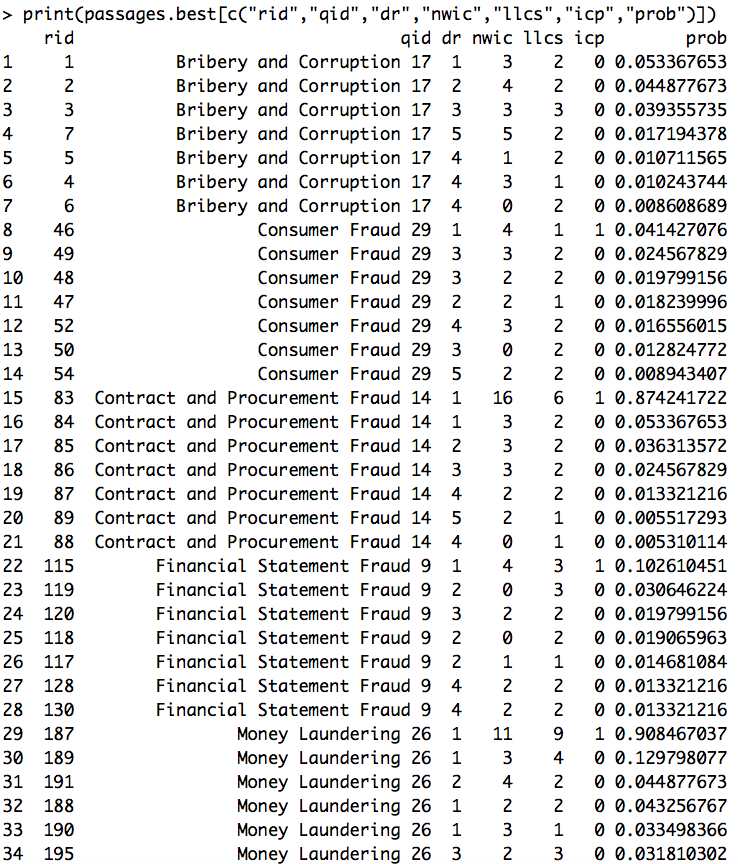
\includegraphics[width=125mm, height=125mm]{logit_model_test_set_top.png}}
\caption{Application of the Passage Classification Model to the Test Set}
\label{fig:logit_model_test_set_top}
\end{figure}

\begin{figure}
\centering
\vspace{1.0in}
\framebox{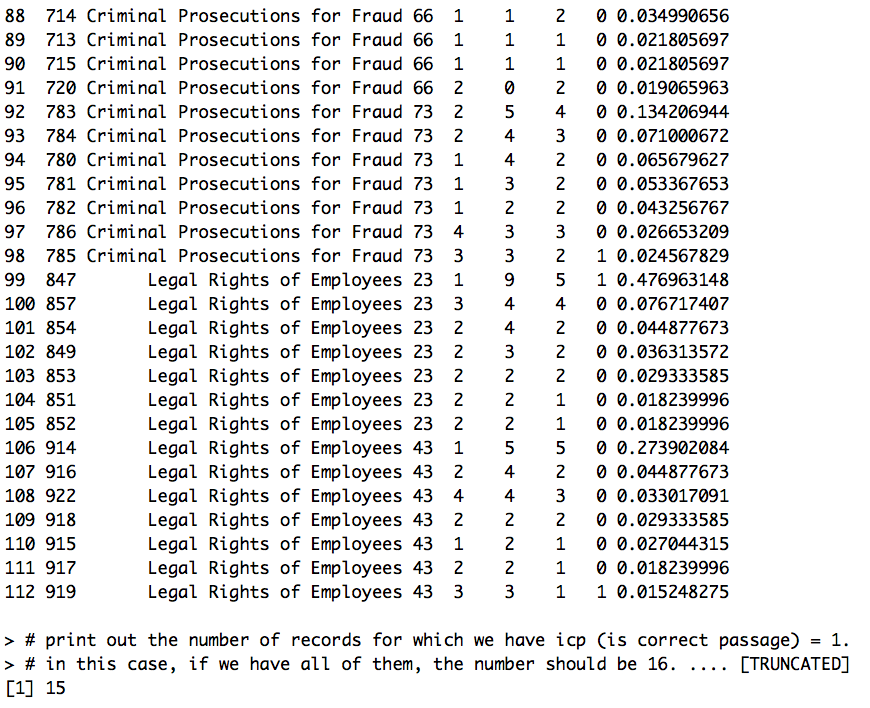
\includegraphics[width=125mm, height=125mm]{logit_model_test_set_bottom.png}}
\caption{Test Set - Count of Correct Passages Retrieved By Classification Model}
\label{fig:test_set_correct_passage_count}
\end{figure}




\section{Answer Processing Algorithms for Version 3}

The answer processing algorithms discussed in this section leverage the top seven passages extracted using the passage classification logistic regression model.  Both of these algorithms are relatively straight-forward in nature and utilize the refined text body in a significant way.  

	% \subsection{Application of the Passage Selection Logit Model}



		% using lucene, as in chapter 04, to get likely documents, and 
		% the passages within 
		% them.
		
		% apply the logit model to determine the probability of being 
		% the correct passage for each passage among the likely documents.
		% rank the passages in order of decreasing probability.
		% select the top 7 passages.

		% \subsubsection{Performance of Passage Selection Logit Model}
		
\subsection{MLPassage1}

MLPassage1 essentially uses the same Max Joint Probability algorithm used in Version 1.  That is, this algorithm calculates the geometric mean frequency of the words in each answer option within the text body for the question.  Except this time, of course, the text body is much more refined to the question.  We see an example of MLPassage1 in Fig.~\ref{fig:mlpassage1_test_case_correct}, where this algorithm successfully selects the correct answer.  We also see its justification for its selection by virtue of the computations of the geometric mean and its selection of the option with the highest value.  However, we are also reminded in this justification that the text body on which it is performing these calculation results from a logistic regression model whose justification is, at best, opaque.  



\begin{figure}
\centering
\vspace{1.0in}
\framebox{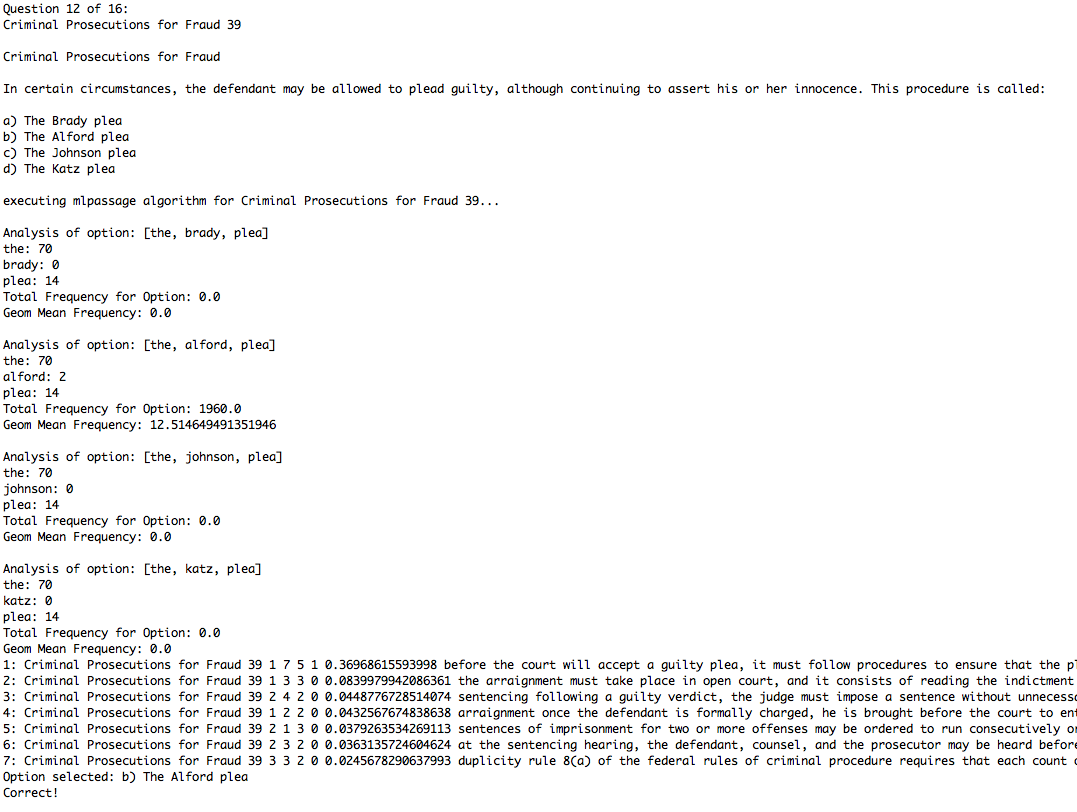
\includegraphics[width=125mm, height=125mm]{mlpassage1_test_case_correct.png}}
\caption{MLPassage1 Algorithm - Test Case 1}
\label{fig:mlpassage1_test_case_correct}
\end{figure}

\subsubsection{MLPassage1 Performance}

For the test set of 16 questions, this algorithm answered 8 questions correctly, 50\%.  Despite the refined approach to selecting passages, this algorithm did not perform up to expectations.  Reasons for this are discussed below.


For a number of other questions in the test set, the algorithm failed to select the correct answer, as shown in the Fig.~\ref{fig:mlpassage1_test_case_incorrect}.  As shown in the answer justification, the problem here stems from the fact that because there is no smoothing (such as, Laplace smoothing) of word frequencies, those options with at least one word that does not occur in the narrowly focused text body are assigned a score of zero.  In the case of the example shown here, the word, ``scam" does not appear anywhere in the text body, and thus all options are assigned a score of zero since all of them include the word ``scam".  Other problems are made apparent in the test set, as well.  MLPassage1 also includes no stemming of the words in order to account for word transformations between the options and the text body.  

Finally, we must remember that only one of the passages is actually considered the correct passage among the seven passages extracted by the passage classification model.  The other six are not relevant.  To the extent MLPassage1 includes all of the passages in its text body for each question, these other six may have a deleterious effect on the performance of the algorithm.  The next algorithm takes this phenomenon into account by using only the first passage among the seven (that is, the passage with highest probability of relevance).

\begin{figure}
\centering
\vspace{1.0in}
\framebox{\includegraphics[width=160mm, height=170mm]{mlpassage1_test_case_incorrect.png}}
\caption{MLPassage1 Algorithm - Test Case 2}
\label{fig:mlpassage1_test_case_incorrect}
\end{figure}


\subsection{MLPassage2}

MLPassage2 addresses two of the problems cited with MLPassage1, namely the stemming problem and the passage selection problem.  An implementation of the Porter Stemmer algorithm was incorporated into this algorithm to address the first issue.  As for the second, this algorithm includes only the first text passage out of the seven.  As noted above, the passage classification algorithm has good precision.  So, reducing the text body to only the first passage would appear to be a prudent decision.  The results bear this out -- With these modifications, the MLPassage2 algorithm shows improved performance of 11 of 16 correct (68.75\%), as shown in Fig.~\ref{fig:mlpassage2_performance}.  

The performance of MLPassage2 is comparable to that seen in Version 2 of the agent on definition questions.  In other words, we see, here, that more complexity doesn't necessarily translate to better accuracy.   After all, we've incorporated another step, using machine learning, which performs its function quite well.  Yet, that alone is not enough to translate to a better score on the exam questions.  There is more room for enhancements and modifications to MLPassage2, however, which should result in better performance with further research.  

\begin{figure}
\centering
\vspace{1.0in}
\framebox{\includegraphics[width=100mm, height=15mm]{mlpassage2_performance.png}}
\caption{MLPassage2 Algorithm Performance}
\label{fig:mlpassage2_performance}
\end{figure}





















 % chapter 5 - Intelligent Agent - Version 3
%%%%%%%%%%%%%%%%%%%%%%%%%%%%%%%%%%%%%%%%%%%%%%%%%%%%%%%%%%%%%%%%%%% 
%                                                                 %
%                            CHAPTER SIX  - Toward a Model for Fraud            %
%                                                                 %
%%%%%%%%%%%%%%%%%%%%%%%%%%%%%%%%%%%%%%%%%%%%%%%%%%%%%%%%%%%%%%%%%%% 
 
\chapter{Version 4 -- Toward a Formal Model for Fraud Detection}

\blfootnote{Portions of this chapter previously appeared as: \bibentry{johnson2014three}} 

In this chapter, we attempt to lay the groundwork for the rigorous study of fraud detection.  Our goal is to not to build an agent in the same sense as Versions 1, 2, and 3 of the CFE Agent whose performance is to be evaluated against CFE exam questions in the spirit of psychometric AI, but instead to build a model that demonstrates a formalized approach to the domain of fraud detection, whereby through formal reasoning, we can answer questions with logico-deductive proof-based justifications.  Furthermore, our ambition in this chapter is not to create a \emph{comprehensive} formal model, but to demonstrate the technique on an examplar subdomain - the detection of doctor shopping.

%% need to attribute these two paragraphs below - taken from the bounded rationality
%% paper.
Included in this chapter is an analysis of the doctor shopping fraud activity in which we present a computational model of doctor shopping in terms of a formal description of the behavior of the perpetrator and the doctors he targets in perpetrating this fraud activity using the $\mathcal{DCEC}^\ast$ \cite{mgmmm_ptai_sb,ka_sb_scc_seqcalc}.  The $\mathcal{DCEC}^\ast$ provides a framework for modeling the interactions of agents in multi-agent systems with respect to their knowledge, beliefs, perceptions, plans, and natural-language capacity.  The syntax and inference rules of the $\mathcal{DCEC}^\ast$ are described in detail in \cite{mgmmm_ptai_sb,ka_sb_scc_seqcalc}; this machinery will be used heavily here.  We specifically use the version of the $\mathcal{DCEC}^\ast$ described in \cite{ka_sb_scc_seqcalc}.

The modeling is done in the Slate \cite{Slate_at_CMNA08} graphical proof-construction environment, where proof verification and proof discovery can be accomplished in an easy-to-use modality.  Slate is based on natural deduction, and includes support for constructing proofs in propositional logic, first-order logic ($\mathcal{FOL}$), and several modal logics.  Slate also has the ability to automatically discover proofs via resolution, by calling ATPs; for example, SNARK \cite{snarksri}.  This feature allows one to utilize Slate in a hybrid mode to construct proofs that are semi-automated.  Slate is ultimately based on a mathematical model of computation and reasoning that is a generalization and extension of Kolmogorov-Uspenskii machines \cite{kolmogorov1958definition,bringsjord_sundar_g_unprov_ct}.


\section{An Example Subdomain - Doctor Shopping}

Doctor shopping is the illegal activity of procurring multiple prescriptions from multiple doctors for the purpose of abuse or illicit profit.  In some cases, the doctors are unaware that the patient has procurred the same prescriptions being sought from other doctors.  In other cases, doctors are co-conspirators.  In this example, we focus on the case in which the patient is the sole perpetrator and the doctors are unaware of his illicit activity.  The CFE Manual describes doctor shopping briefly as follows:

\blockquote{Doctor/ER Shopping: 
Excessive drug claims for controlled substance drugs. Patient “shops” for controlled 
substance drugs. One physician does not know that the other has prescribed the drug. In 
addition, the patient may shop for drugs in emergency rooms complaining of soft tissue 
injuries, sprains, and strains.\cite{acfe_manual_2011_doctorshopping}}

In the development of our formal model for this subdomain, our perspective is that of a fraud examiner; that is, an agent whose purpose is to detect doctor shopping, and to provide justification for its reasoning.  Formal reasoning models provide transparent justifications in the form of applications of inference rules from axioms and declarations pertaining to the problem domain.  We present axioms for the doctor shopping subdomain, and follow them with declarations for a particular example related to this subdomain, below.

Before presenting the formal axioms, though, we need to make note that any formal definition of fraud must include the notion of intent.  It is not sufficient to define fraud in terms of a sequence of actions or events.  For example, it's possible that an patient innocently seeks a prescription from a second doctor simply because he decided he did not like the first doctor he saw for a particular ailment and also, lost the script the first doctor gave him, (pretending for the moment, we're in the pre-modern age of say, 10 years ago when electronic communication of prescriptions was not ubiquitous).  Fraud inherently involves the intent of one party to deceive another for the purpose of personal gain.  And intent implies knowledge.  Thus, the definition of any fraud must inherently involve assertions about cognitive states concerning knowledge and belief on the part of the actors involved.  This is where the use of the $\mathcal{DCEC}^\ast$ comes in handy, as we'll see in the following axioms.

\subsection{Doctor Shopping Axioms}

The first axiom poses a definition of doctor shopping as follows:  Any person, $x$, is guilty of doctor shopping if and only if there exist two doctors, $d1$ and $d2$, such that $x$ knows he gets a prescription, $r$, for duration, $dur$, from $d2$ at time $t2$ while he knows he was already given the same prescription by doctor, $d1$, at time, $t1$, where $t1$ is prior to $t2$ and where the time between $t1$ and $t2$ is short relative the duration of the prescriptions.  (In this case, we arbitrarily specify ``short" as less than 10\% of the prescription duration).  The spirit of this definition is to capture those activities in which the perpetrator is extracting relatively large prescriptions in short order from multiple doctors.  It does not, however, attempt to cover, say, addicts who shop from doctor to doctor looking for prescriptions of short duration simply to support their addiction - (this sort of behavior is emph{also} sometimes referred to as doctor shopping.)  A formal expression of the first axiom is as follows:

%% Axiom1
%% A person, x, is guilty of doctor shopping iff there exists two doctors, d1 and d2 
%% such that x knows he gets an rx from d2 at time t2 while he knows he was 
%% already given an rx from d1 at time t1 (t1 prior to t2) for a
%% where the time between t1 and t2 is small relative the duration of the rx's.

\begin{footnotesize}
\begin{align*}
[A1] \ \forall x . \ &(guilty(x, \Doctorshopping)) \Leftrightarrow \\
	& \exists r, \done, \dtwo, dur, \tone, \ttwo . \ (\knows(x,\happens(\action(x, \getrx(r, \done, dur)), \tone)) \\
	& \wedge \knows(x,\happens(\action(x,\getrx(r,\dtwo,dur)),\ttwo)) \\
	& \wedge \believes(x,\neg\knows(\dtwo,\happens(action(x,\getrx(r,\done,dur)),\tone))) \\
	& \wedge \prior(\tone, \ttwo) \\
	& \wedge \duration(\tone, \ttwo) < dur \times 0.10
\end{align*}
\end{footnotesize}


Our first axiom provides a narrow but fine-grained definition of doctor shopping not only in terms of action but also in terms of the cognitive states of our perpetrator and his unwitting accomplices.  However, for our fraud examiner agent, detecting mental states can be problematic as the data presented, whether it be from a medical claims database or a scenario described in natural language text, often does not provide that level of detailed information.  This leaves our agent having to make some assumptions about the mental state of our perpetrator.  So, our agent makes a general assumption of sound mind -- that is, if an actor commits an act, she is aware, or knows, she is committing that act.  Hence, we have the second axiom given below, that states that if a person, x, gets a prescription of of duration, r, from doctor, d, at time t, he knows he's getting that prescription.

%% Axiom2
%% if x gets a prescription at t, then x knows x gets a prescription at t.

\begin{footnotesize}
\begin{align*}
[A2] \ \forall x, r, d, dur, t . \ &(\happens(\action(x, \getrx(r, d, dur)), t) \Rightarrow \\
& \knows(x,(\happens(\action(x,\getrx(r,d,dur)), t))))
\end{align*}
\end{footnotesize}

In keeping with the general assumption of sound mind, we pose the third axiom, which states that if a patient does not tell a second doctor, $d2$, at time $t2$, that he already received a prescription, $r$, from doctor, $d1$, at time, $t1$, where $t1$ is prior to $t2$, then he knows does not do so.  To emphasize, we're making the assumption, here, that such behavior doesn't arise by accident due to sheer absent-mindedness, but instead due to a deliberate attempt to deceive.

%% Axiom3
%% if x does not tell a doctor that he was already given an rx from another doctor, then he
%% knows he does not tell that doctor that he was already given an rx from another doctor. 

\begin{footnotesize}
\begin{align*}
[A3] \ \forall x, r, &\done, \dtwo, dur, \tone, \ttwo . \ \neg \happens(\action(x,\tells(\dtwo,\happens(\action(x,\getrx(r,\done,dur)),\tone))),\ttwo) \\
& \wedge \prior(\tone,\ttwo) \wedge \done \neq \dtwo \Rightarrow \\
& \knows(x, \neg \happens(\action(x,\tells(\dtwo,\happens(\action(x,\getrx(r,\done,dur)),\tone))),\ttwo))
\end{align*}
\end{footnotesize}


\subsection{Doctor Shopping - An Example}

Suppose we have the following scenario:
\blockquote{Blue gets a prescription from Dr. White on Wednesday for 90 day supply of escitalopram (lexapro) 10mg.  Blue gets a second prescription from Dr. Black on Friday of the same week for the same medication.  Blue does not tell Dr. Black he received the prescription from Dr. White.  Blue believes that if he does not tell Dr. Black about the prescription from Dr. White, then Dr. Black does not know about the prescription from Dr. White.  Is Blue guilty of doctor shopping?}

We'd like the agent to utilize its formal model for doctor shopping to determine the answer to this question.  It should be noted, however, that this kind of question is one that Versions 1, 2, and 3 of the CFE Agent are not designed to handle particularly well since the stem of the question cannot be traced back to a yes or no answer to this question (with any meaningful justification) by referring to the CFE manual.  A formal representation of this problem, in conjunction with the axioms for doctor shopping allow our agent to reason on a semantic level not provided for in our prior versions of the agent, however.  Of course, getting from a natural language representation of the problem domain to a formal representation continues to be an outstanding problem for research, as will be discussed in Chapter 7.  For now, however, we simply move forward with assuming this bridge has been crossed, by simply asserting the formal declarations that represent the semantics of the problem using the $\mathcal{DCEC}^\ast$.

This first declaration deals with Blue getting a 90-day prescription for Lexapro from Dr. White on Wednesday: 

%% Declaration1
%% Blue gets a 90-day prescription for Lexapro from Dr. White on Wednesday
\begin{footnotesize}
\begin{align*}
[D1] \ \happens(\action(\Blue,\getrx(\Lexapro,\DrWhite,90)),\Wednesday)
\end{align*}
\end{footnotesize}

\noindent Next, we have a similar declaration for Blue getting a 90-day prescription for Lexapro from Dr. Black on Friday:
%% Declaration2
%% Blue gets a 90-day prescription for Lexapro from Dr. Black on Friday
\begin{footnotesize}
\begin{align*}
[D2] \ \happens(\action(\Blue,\getrx(\Lexapro,\DrBlack,90)),\Friday)
\end{align*}
\end{footnotesize}

\noindent For our third declaration, we formally represent the assertion that Blue does not tell Dr. Black on Friday that he received a 90-day prescription for Lexapro from Dr. White on the prior Wednesday.
%% Declaration3
%% Blue does not tell Dr. Black on Friday that he received a 90-day prescription 
%% for Lexapro on the prior Wednesday.
\begin{footnotesize}
\begin{align*}
[D3] \ \neg\happens(&\action(\Blue,\tells(\DrBlack, \\
	& \happens(\action(\Blue,\getrx(\Lexapro,\DrWhite,90)),\Wednesday))),\Friday)
\end{align*}
\end{footnotesize}

\noindent And finally, we have a declaration that asserts Blue believes that if he does not tell Dr. Black about the prescription from Dr. White during his visit with Dr. Black on Friday, then Dr. Black does not know Blue received the prescription from Dr. White the preceding Wednesday.
%% Declaration4
%% Blue believes that if he does not tell Dr. Black about the prescription from Dr. White
%% that Dr.Black does not know about the prescription from Dr. White.
\begin{footnotesize}
\begin{align*}
[D4] \ \believes(\Blue,(\neg&\happens(\action(\Blue,\tells(\DrBlack,\\
	& \happens(\action(\Blue,\getrx(\Lexapro,\DrWhite,90)),\Wednesday))),\Friday) \Rightarrow \\
	& \neg\knows(\DrBlack,\happens(\action(\Blue,\getrx(\Lexapro,\DrWhite,90)),\Wednesday))
\end{align*}
\end{footnotesize}

\subsection{Doctor Shopping Proof}

These declarations and the axioms for doctor shopping are sufficient for our agent to prove (and provide justification for its reasoning) that Blue is indeed guilty of doctor shopping.  We walk through the proof in the following paragraphs, step by step.


%% Conclusions

First, the agent uses [$A2$] and [$D1$] to prove that Blue knows he was given a prescription by Dr. White on Wednesday, as shown in Fig.~\ref{fig:proof_of_c1}.  Formally, this conclusion is stated as follows:
%% Conclusion1
%% Blue knows he gets a 90-day prescription for Lexapro from Dr. White on Wednesday
\begin{footnotesize}
\begin{align*}
[C1] \ \knows(\Blue,\happens(\action(\Blue,\getrx(\Lexapro,\DrWhite,90)),\Wednesday))
\end{align*}
\end{footnotesize}

%%++++++++++++++++++++++++++++++++++++++++++++++++++++++++++++++++++++
\begin{figure}[h!] 
\vspace{6pt}
\centering
\framebox{\includegraphics[width=1.0\textwidth]{c1_proof.png}}
\caption{Proof of $C1$ -- Blue knows he was given a prescription by Dr. White on 
Wednesday.}
\label{fig:proof_of_c1}
\end{figure}
%%++++++++++++++++++++++++++++++++++++++++++++++++++++++++++++++++++++

\noindent Next, the agent uses [$A2$] and [$D2$] to prove Blue also knows he was given a prescription by Dr. Black on Friday, as shown in Fig.~\ref{fig:proof_of_c2}, which stated formally, is as follows:
%% Conclusion2
%% Blue knows he gets a 90-day prescription for Lexapro from Dr. Black on Friday
\begin{footnotesize}
\begin{align*}
[C2] \ \knows(\Blue,\happens(\action(\Blue,\getrx(\Lexapro,\DrBlack,90)),\Friday))
\end{align*}
\end{footnotesize}

%%++++++++++++++++++++++++++++++++++++++++++++++++++++++++++++++++++++
\begin{figure}[h!] 
\vspace{6pt}
\centering
\framebox{\includegraphics[width=1.0\textwidth]{c2_proof.png}}
\caption{Proof of $C2$ -- Blue knows he was given a prescription by Dr. Black on 
Friday.}
\label{fig:proof_of_c2}
\end{figure}
%%++++++++++++++++++++++++++++++++++++++++++++++++++++++++++++++++++++

\noindent Next, the agent uses [$A3$] to prove the conditional statement that if Blue does not tell Dr. Black about the prescription he received from Dr. White, then he \emph{knows} he does not tell him, stated formally in [C3] below.  The proof is shown in Fig.~\ref{fig:proof_of_c3}.

%% Conclusion3
%% If Blue doesn't tell Dr. Black on Friday that he received a prescription for 90 days Lexapro
%% from Dr. White on Wednesday, then he **knows** he didn't tell him this.
\begin{footnotesize}
\begin{align*}
[C3] \ \neg \happens&(\action(\Blue,\tells(\DrBlack,\\
& \happens(\action(\Blue,\getrx(\Lexapro,\DrWhite,90)),\Wednesday))),\Friday) \\
& \wedge \prior(\Wednesday,\Friday) \wedge \DrWhite \neq \DrBlack \Rightarrow \\
& \knows(\Blue, \neg \happens(\action(\Blue,\tells(\DrBlack,\\ 
& \happens(\action(\Blue,\getrx(\Lexapro,\DrWhite,90)),\Wednesday))),\Friday))
\end{align*}
\end{footnotesize}

%%++++++++++++++++++++++++++++++++++++++++++++++++++++++++++++++++++++
\begin{figure}[h!] 
\vspace{6pt}
\centering
\framebox{\includegraphics[width=1.0\textwidth]{c3_proof.png}}
\caption{Proof of $C3$ -- If Blue does not tell Dr. Black about the prescription he received from Dr. White then Blue knows he does not tell him.}
\label{fig:proof_of_c3}
\end{figure}
%%++++++++++++++++++++++++++++++++++++++++++++++++++++++++++++++++++++



\noindent Next, the agent uses [$C3$], [$D3$], and [$D4$] to prove the assertion that Blue believes that Dr. Black does not know about the fact he reeived a prescription from Dr. White on Wednesday, as represented formally by [$C4$], shown below.  This proof is shown in Fig.~\ref{fig:proof_of_c4}.  Also required by this proof are two supporting declations -- one about the order of occurence of Wednesday and Friday in a given week and another that asserts that $DrBlack$ and $DrWhite$ are constants referencing different objects (doctors, actually) in the problem domain.

%% Conclusion4
%% Blue believes Dr. Black does not know that Blue received a 90-day prescription for 
%% Lexapro on Wednesday
\begin{footnotesize}
\begin{align*}
[C4] \ \believes(\Blue, \neg \knows(\DrBlack,\happens(\action(\Blue,\getrx(\Lexapro,\DrWhite,90)),\Wednesday)))
\end{align*}
\end{footnotesize}

%%++++++++++++++++++++++++++++++++++++++++++++++++++++++++++++++++++++
\begin{figure}[h!] 
\vspace{6pt}
\centering
\framebox{\includegraphics[width=1.0\textwidth]{c4_proof.png}}
\caption{Proof of $C4$ -- Blue believes that Dr. Black does not know he received a prescription from Dr. White on Wednesday.}
\label{fig:proof_of_c4}
\end{figure}
%%++++++++++++++++++++++++++++++++++++++++++++++++++++++++++++++++++++


\noindent Finally, using [$A1$], [$C1$], [$C2$], and [$C4$], the agent proves Blue is guilty of doctor shopping.  As was the case for the proof of [$C4$], the proof also requires supporting declarations related to time and the number of days between Wednesday and Friday relative to 10\% of the prescription duration.  This proof is shown in Fig.~\ref{fig:proof_of_c5}.
%% Conclusion5
%% Blue is guilty of doctor shopping.
\begin{footnotesize}
\begin{align*}
[C5] \ \guilty(\Blue,\Doctorshopping)
\end{align*}
\end{footnotesize}


%%++++++++++++++++++++++++++++++++++++++++++++++++++++++++++++++++++++
\begin{figure}[h!] 
\vspace{6pt}
\centering
\framebox{\includegraphics[width=1.0\textwidth]{c5_proof.png}}
\caption{Proof of $C5$ -- Blue is guilty of doctor shopping.}
\label{fig:proof_of_c5}
\end{figure}
%%++++++++++++++++++++++++++++++++++++++++++++++++++++++++++++++++++++

Taken together, these proofs add up to a completely transparent justification of the agent's reasoning for its ultimate conclusion that Blue is guilty of doctor shopping.  As mentioned earlier, this level of transparency is a feature of this formal, semantic approach that the approaches of Versions 1, 2, and 3 do not offer.  However, there are costs to this approach as well, as the reader may have noted during the walk through of the proof.  First, natural language assertions must be translated into a formal language, as mentioned earlier.  And second, the model must be constructed such that it is comprehensive enough for the agent to make the necessary inferences it needs to complete the proof.  Niether of these is an easy task.  Often, assertions must be constructed based on common-sense-based real world knowledge, and are not explicitly stated in the text of supporting documentation or the scenario description.  Further discussion of these issues as well as the merits and pitfalls of the approaches we've seen to this point in the development of the CFE agent will be continued in Chapter 7.


%% notes 06/09/2016

%1.  any formal definition of fraud must include the notion of intent.  It is not sufficient to define fraud in terms of a sequence of events in which resources are transferred from one party to another.  Fraud inherently involves the intent of one party to deceive another party for the purpose of gaining advantage or resources.  Intent 
%
%2.  intent implies knowledge.  thus, the definition in terms of cognitive states of fraud are steeped in assertions about knowledge.
%
%3.  if knowledge on the part of the suspected fraudster is not known, it is possible that the suspect simply engaged in a sequence of actions that might appear to be fraud but don't amount to fraud.  For example, what if, on the second attempt to procure an rx, the suspect, for whatever reason, was unaware that he already was given the rx.  For example, consider a situation in which the suspect gets a script for an rx, takes it home, but then loses it because his wife mistakenly throws it in the garbage.  Because he's traveling on business, he quickly goes to an out-of-town doctor who does not know the first doctor, and gets the same rx in order to replace the lost script.  This is clearly not fraud, but the fact that he goes to two doctors in quick succession to get the same rx would appear to be fraud.
%
%4.  However, how can a machine imbued with these extremely fine-grained definitions of fraud in relation to fine-grained mental states detect the mental states of all parties involved, most importantly the fraudster?  It can't.  Thus we need to make assumptions about mental states.  Specifically, we assume that the suspect, if he gets an rx, knows he's getting it, and doesn't forget that he got it when he gets the second one.  In other words, we assume the worst for the suspect, even though there are plausible circustances in which the suspect would not know, as discussed above.


%%\section{A First Example - The Law Related to Fraud 39}
%%
%%Fig.~\ref{fig:law_related_to_fraud_39_question} shows the first example we consider.  This question qualifies as a definition-type question, centering on the concept of larceny.  In order get this question correct, one must recognize that larceny is essentially synonymous with theft, or, pertinent to this question, stealing.  From this fact we make the following assertion regarding committing larceny in terms of stealing:
%%
%%\begin{footnotesize}
%%\begin{align*}
%%%%[A1] \ \forall t, a, x. \ & \happens(action(a, \bids(x+1), t+1)) \\ 
%%%%	& \Rightarrow \holds(highbid(x), t) \wedge \neg \holds(highbidder(a), t))
%%\end{align*}
%%\end{footnotesize}

%\begin{figure}
%\centering
%\vspace{1.0in}
%\includegraphics[width=100mm, height=50mm]{law_related_to_fraud_39_question.png}
%\caption{Law Related to Fraud 39}
%\label{fig:law_related_to_fraud_39_question}
%\end{figure}
%
%
%\begin{figure}
%\centering
%\vspace{1.0in}
%\includegraphics[width=50mm, height=60mm]{law_related_to_fraud_39_1.png}
%\caption{Law Related to Fraud 39 - Proof of Correct Answer (Larceny)}
%\label{fig:law_related_to_fraud_39_1}
%\end{figure}
%
%\begin{figure}
%\centering
%\vspace{1.0in}
%\includegraphics[width=50mm, height=100mm]{law_related_to_fraud_39_2.png}
%\caption{Law Related to Fraud 39 - Proof of Incorrect Answer (Embezzlement)}
%\label{fig:law_related_to_fraud_39_2}
%\end{figure}






















 % chapter 6 - Toward a Formal Model for Fraud
%%%%%%%%%%%%%%%%%%%%%%%%%%%%%%%%%%%%%%%%%%%%%%%%%%%%%%%%%%%%%%%%%%% 
%                                                                 %
%                            CHAPTER SEVEN  - Conclusion and Future Work            %
%                                                                 %
%%%%%%%%%%%%%%%%%%%%%%%%%%%%%%%%%%%%%%%%%%%%%%%%%%%%%%%%%%%%%%%%%%% 
 

\chapter{Conclusion and Future Work}

This chapter summarizes the work we’ve covered in this dissertation and offers areas for further investigation.

\section{Summary of Work}

The research in this dissertation began with developing a battery of multiple choice questions from the CFE exam materials and the preparation of the CFE Manual text for test processing by an automated agent. Next, we presented Version 1 of the CFE agent which used very primitive rule-based algorithms to answer questions but which were nonetheless quite effective relative to random guessing, and the results proved statistically significant at the 99\% level. Unfortunately, justifications for the agent’s answers left much to be desired - offering no more justification than that for choosing a particular algorithm based on optimal performance in the training set.  

In Version 2 of the agent, more sophisticated algorithms were brought to bear on the problem using information retrieval for which we saw marked improvement in accuracy (a jump from roughly 49\% accuracy to 59.5\%, and in particular, a 70\% accuracy rate for ConceptMatchV3 on definition questions) and a more (but not completely) transparent justification for the agent’s answers. Here, though, the justifications in the agent’s answers were still not completely transparent as the coefficients upon which the cosine similarity computations were based were derived from digesting term counts within the documents of the document collection. And so, justifications were limited to demonstrating how coefficients determined at the aggregate level were applied to arrive at the answer for each individual question.

Version 3 of the agent used machine learning to isolate the passages (paragraphs) from among the documents in the document collection relevant to each definition question. This technique provided 93\% probability that the correct passage was within the selection of top seven passages as ranked by the logistic regression
algorithm in the test set. Although the relatively simplistic answer extraction algorithms that utilized the results of the passage selection algorithm yielded roughly 69\% accuracy on the definition questions in the test set, we believe further work to refine these answer extraction algorithms will result in significant accuracy gains, surpassing those of Version 2 at a statistically significant level. However, as we saw with Version 2, this approach offered only limited transparency into the reasoning by the agent, limited to the application of opaquely determined coefficients at the aggregate level to each individual problem.

Finally, in Version 4 of the agent, we looked at utilizing semantic reasoning in the agent. This approach offered the benefit of completely transparent reasoning based on natural deduction using the $\mathcal{DCEC}^\ast$.  However, our work here highlighted an important issue with this approach -- the problem of translating assertions expressed in natural language into a formal language, (in our case, again, the language of choice was the $\mathcal{DCEC}^\ast$).  This problem exists for both translating assertions in the information source (the CFE Manual, in our example), and for translating declaration germane to the problem at hand. In the example we covered in Chapter 6, these were the assertions associated with Blue and his interactions with Dr. White and Dr. Black.

\section{Future Work}

Certainly, as alluded to in the above paragraphs, the incorporation of machine learning into passage selection offered considerable promise for refining the algorithms of the CFE agent. So, continuing along this path, further refinement of the answer extraction algorithms would also likely deliver improved overall accuracy, as discussed above. Specifically, perhaps incorporation of machine learning in the answer extraction algorithm as well as the passage selection algorithm may prove beneficial. This is a tact that will be pursued in future work.

Now, consider the following problem from the CFE test set:

\blockquote{True or False: Green, an agent for the White Corporation, acting within the scope of his duties and for the benefit of White, committed an act of fraud. According to the Sentencing Guidelines effective in 1991, White cannot be held criminally liable for Green’s actions.}

This is a true/false question, a type that was not specifically targeted in any of the first three versions of the CFE agent. The reason for that is obvious – this is a tough problem for the CFE Agent using the algorithms of Versions 1, 2, and 3 where the algorithms are looking for the juxtaposition of key words of the question stem and those of the various answer options within the CFE Manual. In a true/false problem, however, answer options are of no help, leaving the agent with only the question stem from which it must discern whether the statement is valid.  Proximity of key words will likely not work here as it is likely that such questions rich with keywords from a given section are as likely to be invalid as valid. (This statement is merely conjecture at this point. Further work needs to be done here to verify this assertion scientifically.)

An algorithm that is based on a semantic understanding of the problem would certainly appear useful, here. But for that, we'd need the tools for translating natural language assertions to ones expressed in a formal language, where in our case, we'd recommend the $\mathcal{DCEC}^\ast$ due to its built-in support for modeling the cognitive states and interactions typical of agents in financial fraud scenarios. There are two possible approaches for tackling this task. The first approach to the translation problem is a computational semantics approach based on Blackburn and Bos \cite{blackburn_2005_representation_ch2}, wherein the authors explain an approach to the representation of natural language assertions in first-order logic ($\mathcal{FOL}$) using the lambda calculus. In the approach we propose here, however, the target representation language would be the $\mathcal{DCEC}^\ast$, not $\mathcal{FOL}$.  A second approach would involve parsing the sentences first, using a probabilistic parser \cite{martin_2000_speech_ch14}, such as OpenNLP (https://opennlp.apache.org) or the Stanford Parser (http://nlp.stanford.edu/software/lex-parser.shtml),  and then translating the parse structures into assertions expressedin the $\mathcal{DCEC}^\ast$.  The idea here is that both the natural language utterances and the parse structures serve as inputs to the computational semantics \cite{blackburn_2005_representation_ch2} model that produces the output assertions in the $\mathcal{DCEC}^\ast$.  Having parse structures as inputs may be helpful in better capturing the semantics of the utterance in the semantics model. 

As a final thought, we believe that any comprehensive QA system that provides both answers with a high degree of accuracy along with justifications, a holistic approach would be required – one that leverages extended versions of the machine learning/information retrieval approaches in Versions 2 and 3 of the agent as well as the semantic approach of Version 4. How might that be accomplished? Depending on the type of question, this holistic approach could take on different forms. For true/false questions, as we have seen, machine learning approaches may be of limited use, and thus an approach more centered around semantic computation is required.  However, for definition questions, a high level approach might be to leverage the machine learning approach to arrive at an answer, and then use that answer to engineer the justification using a semantic approach.  The idea here is to utilize the machine learning approaches for finding the answers and the semantic computational approach for explaining them. For other types of questions, still yet a different blend of these approaches may be required. % chapter 7 - Conclusion and Future Work
%%%%%%%%%%%%%%%%%%%%%%%%%%%%%%%%%%%%%%%%%%%%%%%%%%%%%%%%%%%%%%%%%%% 
%                                                                 %
%                           BIBLIOGRAPHY                          %
%                                                                 %
%%%%%%%%%%%%%%%%%%%%%%%%%%%%%%%%%%%%%%%%%%%%%%%%%%%%%%%%%%%%%%%%%%% 
 
%This method produces a numbered bibliography where the numbers
%correspond to the \cite commands in the text. See the LaTeX manual.
%
\specialhead{REFERENCES}
\bibliographystyle{ieeetr}
\begin{singlespace}
\bibliography{joebib,main72,naveen}
\end{singlespace}


%\begin{singlespace}
%\begin{thebibliography}{99}
%\bibitem{thisbook} This is the first item in the Bibliography.
%Let's make it very long so it takes more than one line.
%Let's make it very long so it takes more than one line.
%Let's make it very long so it takes more than one line.
%Let's make it very long so it takes more than one line. 
%\bibitem{anotherbook} The second item in the Bibliography.
%\bibitem{yetanotherbook} Another item in the Bibliography.
%\end{thebibliography}
%\end{singlespace}

% Note that, if you wish, you can use BibTeX to create your bibliography
% from a database. See section 5.6.2 of Memo RPI.110 for information. 
%%% Local Variables: 
%%% mode: latex
%%% TeX-master: t
%%% End: 
 % bibliography
%%%%%%%%%%%%%%%%%%%%%%%%%%%%%%%%%%%%%%%%%%%%%%%%%%%%%%%%%%%%%%%%%%%
%                                                                 %
%                            APPENDICES                           %
%                                                                 %
%%%%%%%%%%%%%%%%%%%%%%%%%%%%%%%%%%%%%%%%%%%%%%%%%%%%%%%%%%%%%%%%%%%
 
\appendix    % This command is used only once!
%\addcontentsline{toc}{chapter}{APPENDICES}             %toc entry  or:
\addtocontents{toc}{\parindent0pt\vskip12pt APPENDICES} %toc entry, no page #

\chapter{Brief Overview of Information Retrieval}
\label{app:information_retrieval}

Information Retrieval (IR) \cite{manning_2008_introduction_ch1} is the branch of AI dealing with the creation of software that retrieves documents of an unstructured nature from among a large collection of documents in response to an information need expressed as a natural language query.   A document is a unit of data, typically unstructured or semi-structured, and typically expressed in natural language.  (One of the fundamental questions to consider in IR is how to define a document - a sentence? a paragraph? a chapter?  The answer typically depends on the nature of the problem domain.)  A document collection is simply a collection of such documents, as defined above.  Finally, a vocabulary, $V=\{t_1,t_2,t_3,...,t_n\}$ is the set of all terms over which the contents of the documents are defined.

\section{Boolean Retrieval}

Boolean information retrieval is based on the idea of dividing up the document collection into two sets for each query - one set of documents which meets the requirements of the boolean query and the other set whose documents does not.  Boolean queries are structured as conjunctions of disjunctions; that is, of the form of query, $q$, where

%\begin{gather*}
%q = (W_i \lor W_k \lor ...) \land ... \land (W_j \lor W_s \lor ...) \\
%\textrm{where}\ W_i = t_i, W_k = t_k, W_j = t_j, W_s = t_s, \\
%\textrm{or}\ W_i = NON\ t_i, W_k = NON\ t_k, W_j = NON\ t_j, W_s = NON\ t_s \\
%\text{where $t_i$ means that $t_i$ exists in the document and $NON\ t_i$ means it does not}
%\end{gather*}

\begin{equation}
q = (W_i \lor W_k \lor ...) \land ... \land (W_j \lor W_s \lor ...) \\
\end{equation}
where $W_i = t_i, W_k = t_k, W_j = t_j, W_s = t_s,$ or $W_i = NON\ t_i, W_k = NON\ t_k, W_j = NON\ t_j, W_s = NON\ t_s$ and where $t_i$ means that $t_i$ exists in the document and $NON\ t_i$ means it does not \cite{wiki:boolean_retrieval}.

%q = (Wi OR Wk OR ...) AND ... AND (Wj OR Ws OR ...)
%
%where Wi=ti, Wk=tk, Wj = tj, Ws = ts, or Wi = NON ti, Wk = NON tk, or Wj = NON tj, or Ws = NON ts, 
%
%where ti indicates the term ti is present in the doucument and NON ti indicates it is not.

\subsection{Term-Document Incidence Matrix}

Boolean retrieval may be  implemented using a data structure called a term-document incidence matrix, $A$, where $A$ is a two-dimensional array in which the $i$th row denotes the $i$th document in the document collection and where $j$th column denotes the $j$th term in the vocabulary, and where $A[i,j] = 1$ if the term, $i$ exists in the document, $j$, and 0 otherwise.  Based on $A$, the processing of a query involves finding those documents for which there is a 1 in each of the rows corresponding to the terms of the query \cite{manning_2008_introduction_ch1}.  

A significant pitfall of this method is that it requires a vast amount of memory.  Consider an example consisting of 1 million documents and a vocabulary of 500,000 words.  Then, the size of the matrix is 50 trillion (1 million x 500,000).  This matrix is also highly sparse since any given document has on average a small number of words relative to the size of the vocabulary.  Suppose, for example, each document has 1,000 words.  Then, for each document, among the 50,000 elements in its corresponding row of the matrix, only 1,000 (2\%) are non-zero \cite{manning_2008_introduction_ch1}.	

\subsection{Inverted Index}

An alternative implementation for boolean retrieval utilizes an inverted Index -- a hash table in which the keys are the terms in the vocabulary and the value is a linked list of all of the identifiers for those documents in which that term appears.  This technique exploits the sparsity of the term-document matrix -- requiring memory only for those elements in which $A(i,j) = 1$ \cite{manning_2008_introduction_ch1}.


\section{Ranked Retrieval}

Boolean retrieval has the unfortunate drawback of returning a set of documents in response to a query as a set of equally ranked units through which the user must sift in order to find the information sought \cite{manning_2008_introduction_ch6}.  Sometimes, this sifting can be a sizable task depending on the number of documents returns from the boolean query.  Ranked retrieval, on the other hand, is IR in which documents are ranked according to a score that measure the degree of similarity between the query and the terms of the document and in which documents are returned in decreasing sorted order of this score \cite{manning_2008_introduction_ch6}.  

The Vector Space model (VSM) \cite{manning_2008_introduction_ch6} is one approach to ranked retrieval, and is based on representing the documents in the collection and the query as vectors and where documents are scored according to a measure of similarity between their vector representations and that of the query.  There are a number of measures, or weights, that are typically incorporated into a vector representation as discussed below.

The log of the term frequency, $\textrm{log}_{10}(tf)$ is a measure of the number of occurences of a particular term in the document.  (The log is used as opposed to the term frequency, itself, in order to dampen the effect for each additional occurrence of a term.)  The log-frequency weight of term, $t$ in document, $d$ is given by \cite{manning_2008_introduction_ch6}:

\begin{equation}
w(t,d) = 1 + \textrm{log}_{10}(tf_d), \textrm{where}\ tf_d > 0, 0\  \textrm{otherwise}
\end{equation}

Inverse document frequency is a measure of the relative scarcity of a term in a document relative to the other documents in the collection.  A higher weight is assigned to a term that appears in relatively few documents compared with one that appears in many.  The inverse document frequency, $idf(t)$, can be calculated for each term, t, of the query as follows \cite{manning_2008_introduction_ch6}:  

\begin{equation}
idf(t)  = \textrm{log}_{10}(N/df_t),
\end{equation}

\noindent
where $N$ is the number of documents in the collection and $df_t$ is the number of documents containing term, $t$.  Again, as is the case for term frequency, the log is used here to moderate the effect of the measure.

We can combine these two measures such that for each term, $t$, in each document, $d$, we have \cite{manning_2008_introduction_ch6}:

\begin{equation}
w(t,d) = (1 + \textrm{log}_{10}(tf_d)) \times \textrm{log}_{10}(N/df_t).
\end{equation}

\noindent
The vector representation of a document, $d$, is $\vec{d}$, where

\begin{equation}
\vec{d} =  [w(t_1,d), w(t_2,d), w(t_3,d),...., w(t_n, d)], 
\end{equation}

\noindent
where, as defined above our vocabulary, $V=\{t_1,t_2, ..., t_n\}$.  Note, queries can also be vectorized in the same way.  

In order to measure the relative relevance of document, $d$, to the query, $q$, the vector representations of both $d$ and $q$, $\vec{d}$ and $\vec{q}$, are harnessed to compute a quantitative measure of the level of similarity between the two vectors using the concept of cosine similarity.  Informally, the cosine similarity of two n-dimensional vectors is a measure of the cosine of the angle between them in n-dimensional space.  Normalization of the lengths of the vectors is also incorporated into this calculation to assure that longer documents' weights do not outsize the weights of shorter (but perhaps, similar) documents, (such as the query itself, which is commonly much shorter than the document against which it is compared).  

\begin{equation}
\begin{split}
\textrm{sim}(q, d) & = \dfrac{\vec{q} \cdot \vec{d}}{|\vec{q}||\vec{d}|} \\
 & = \dfrac{\vec{q}}{|\vec{q}|} \cdot \dfrac{\vec{d}}{|\vec{d}|}
\end{split}
%	= q(arrow)/length(q(arrow)) dot d(arrow)/length(d(arrow)) = 
%	= sum(i to length(V))q(i)d(i)/(sum(i to length(V)q(i)\^2))(sum(i to length(V)d(i)\^2))
\end{equation}

\noindent
For a document, $d$ whose length-normalized-vector representation is similar to that of $q$, the angle between its vector and that of $q$ should be small (close to 0), and thus have a cosine near 1.  For those documents not similar to $q$, the cosine measure will tend toward 0, (note that all of the terms in these vector-representation vectors are greater than or equal to 0).  Under the document vectorization approach, the highest $K$ documents are returned in response to a query, $q$, in order of decreasing cosine similarity, where $K$ is an arbitrary figure intended to limit the size of the return set.





 % appendix - information retrieval
%\bibliographystyle{agsm}
%\begin{footnotesize}
%\bibliography{joebib}
%\end{footnotesize}
%%%%%%%%%%%%%%%%%%%%%%%%%%%%%%%%%%%%%%%%%%%%%%%%%%%%%%%%%%%%%%%%%%%%
%                                                                 %
%                            APPENDICES                           %
%                                                                 %
%%%%%%%%%%%%%%%%%%%%%%%%%%%%%%%%%%%%%%%%%%%%%%%%%%%%%%%%%%%%%%%%%%%
 
\appendix    % This command is used only once!
%\addcontentsline{toc}{chapter}{APPENDICES}             %toc entry  or:
\addtocontents{toc}{\parindent0pt\vskip12pt APPENDICES} %toc entry, no page #

\chapter{Brief Overview of Information Retrieval}
\label{app:information_retrieval}

Information Retrieval (IR) \cite{manning_2008_introduction_ch1} is the branch of AI dealing with the creation of software that retrieves documents of an unstructured nature from among a large collection of documents in response to an information need expressed as a natural language query.   A document is a unit of data, typically unstructured or semi-structured, and typically expressed in natural language.  (One of the fundamental questions to consider in IR is how to define a document - a sentence? a paragraph? a chapter?  The answer typically depends on the nature of the problem domain.)  A document collection is simply a collection of such documents, as defined above.  Finally, a vocabulary, $V=\{t_1,t_2,t_3,...,t_n\}$ is the set of all terms over which the contents of the documents are defined.

\section{Boolean Retrieval}

Boolean information retrieval is based on the idea of dividing up the document collection into two sets for each query - one set of documents which meets the requirements of the boolean query and the other set whose documents does not.  Boolean queries are structured as conjunctions of disjunctions; that is, of the form of query, $q$, where

%\begin{gather*}
%q = (W_i \lor W_k \lor ...) \land ... \land (W_j \lor W_s \lor ...) \\
%\textrm{where}\ W_i = t_i, W_k = t_k, W_j = t_j, W_s = t_s, \\
%\textrm{or}\ W_i = NON\ t_i, W_k = NON\ t_k, W_j = NON\ t_j, W_s = NON\ t_s \\
%\text{where $t_i$ means that $t_i$ exists in the document and $NON\ t_i$ means it does not}
%\end{gather*}

\begin{equation}
q = (W_i \lor W_k \lor ...) \land ... \land (W_j \lor W_s \lor ...) \\
\end{equation}
where $W_i = t_i, W_k = t_k, W_j = t_j, W_s = t_s,$ or $W_i = NON\ t_i, W_k = NON\ t_k, W_j = NON\ t_j, W_s = NON\ t_s$ and where $t_i$ means that $t_i$ exists in the document and $NON\ t_i$ means it does not \cite{wiki:boolean_retrieval}.

%q = (Wi OR Wk OR ...) AND ... AND (Wj OR Ws OR ...)
%
%where Wi=ti, Wk=tk, Wj = tj, Ws = ts, or Wi = NON ti, Wk = NON tk, or Wj = NON tj, or Ws = NON ts, 
%
%where ti indicates the term ti is present in the doucument and NON ti indicates it is not.

\subsection{Term-Document Incidence Matrix}

Boolean retrieval may be  implemented using a data structure called a term-document incidence matrix, $A$, where $A$ is a two-dimensional array in which the $i$th row denotes the $i$th document in the document collection and where $j$th column denotes the $j$th term in the vocabulary, and where $A[i,j] = 1$ if the term, $i$ exists in the document, $j$, and 0 otherwise.  Based on $A$, the processing of a query involves finding those documents for which there is a 1 in each of the rows corresponding to the terms of the query \cite{manning_2008_introduction_ch1}.  

A significant pitfall of this method is that it requires a vast amount of memory.  Consider an example consisting of 1 million documents and a vocabulary of 500,000 words.  Then, the size of the matrix is 50 trillion (1 million x 500,000).  This matrix is also highly sparse since any given document has on average a small number of words relative to the size of the vocabulary.  Suppose, for example, each document has 1,000 words.  Then, for each document, among the 50,000 elements in its corresponding row of the matrix, only 1,000 (2\%) are non-zero \cite{manning_2008_introduction_ch1}.	

\subsection{Inverted Index}

An alternative implementation for boolean retrieval utilizes an inverted Index -- a hash table in which the keys are the terms in the vocabulary and the value is a linked list of all of the identifiers for those documents in which that term appears.  This technique exploits the sparsity of the term-document matrix -- requiring memory only for those elements in which $A(i,j) = 1$ \cite{manning_2008_introduction_ch1}.


\section{Ranked Retrieval}

Boolean retrieval has the unfortunate drawback of returning a set of documents in response to a query as a set of equally ranked units through which the user must sift in order to find the information sought \cite{manning_2008_introduction_ch6}.  Sometimes, this sifting can be a sizable task depending on the number of documents returns from the boolean query.  Ranked retrieval, on the other hand, is IR in which documents are ranked according to a score that measure the degree of similarity between the query and the terms of the document and in which documents are returned in decreasing sorted order of this score \cite{manning_2008_introduction_ch6}.  

The Vector Space model (VSM) \cite{manning_2008_introduction_ch6} is one approach to ranked retrieval, and is based on representing the documents in the collection and the query as vectors and where documents are scored according to a measure of similarity between their vector representations and that of the query.  There are a number of measures, or weights, that are typically incorporated into a vector representation as discussed below.

The log of the term frequency, $\textrm{log}_{10}(tf)$ is a measure of the number of occurences of a particular term in the document.  (The log is used as opposed to the term frequency, itself, in order to dampen the effect for each additional occurrence of a term.)  The log-frequency weight of term, $t$ in document, $d$ is given by \cite{manning_2008_introduction_ch6}:

\begin{equation}
w(t,d) = 1 + \textrm{log}_{10}(tf_d), \textrm{where}\ tf_d > 0, 0\  \textrm{otherwise}
\end{equation}

Inverse document frequency is a measure of the relative scarcity of a term in a document relative to the other documents in the collection.  A higher weight is assigned to a term that appears in relatively few documents compared with one that appears in many.  The inverse document frequency, $idf(t)$, can be calculated for each term, t, of the query as follows \cite{manning_2008_introduction_ch6}:  

\begin{equation}
idf(t)  = \textrm{log}_{10}(N/df_t),
\end{equation}

\noindent
where $N$ is the number of documents in the collection and $df_t$ is the number of documents containing term, $t$.  Again, as is the case for term frequency, the log is used here to moderate the effect of the measure.

We can combine these two measures such that for each term, $t$, in each document, $d$, we have \cite{manning_2008_introduction_ch6}:

\begin{equation}
w(t,d) = (1 + \textrm{log}_{10}(tf_d)) \times \textrm{log}_{10}(N/df_t).
\end{equation}

\noindent
The vector representation of a document, $d$, is $\vec{d}$, where

\begin{equation}
\vec{d} =  [w(t_1,d), w(t_2,d), w(t_3,d),...., w(t_n, d)], 
\end{equation}

\noindent
where, as defined above our vocabulary, $V=\{t_1,t_2, ..., t_n\}$.  Note, queries can also be vectorized in the same way.  

In order to measure the relative relevance of document, $d$, to the query, $q$, the vector representations of both $d$ and $q$, $\vec{d}$ and $\vec{q}$, are harnessed to compute a quantitative measure of the level of similarity between the two vectors using the concept of cosine similarity.  Informally, the cosine similarity of two n-dimensional vectors is a measure of the cosine of the angle between them in n-dimensional space.  Normalization of the lengths of the vectors is also incorporated into this calculation to assure that longer documents' weights do not outsize the weights of shorter (but perhaps, similar) documents, (such as the query itself, which is commonly much shorter than the document against which it is compared).  

\begin{equation}
\begin{split}
\textrm{sim}(q, d) & = \dfrac{\vec{q} \cdot \vec{d}}{|\vec{q}||\vec{d}|} \\
 & = \dfrac{\vec{q}}{|\vec{q}|} \cdot \dfrac{\vec{d}}{|\vec{d}|}
\end{split}
%	= q(arrow)/length(q(arrow)) dot d(arrow)/length(d(arrow)) = 
%	= sum(i to length(V))q(i)d(i)/(sum(i to length(V)q(i)\^2))(sum(i to length(V)d(i)\^2))
\end{equation}

\noindent
For a document, $d$ whose length-normalized-vector representation is similar to that of $q$, the angle between its vector and that of $q$ should be small (close to 0), and thus have a cosine near 1.  For those documents not similar to $q$, the cosine measure will tend toward 0, (note that all of the terms in these vector-representation vectors are greater than or equal to 0).  Under the document vectorization approach, the highest $K$ documents are returned in response to a query, $q$, in order of decreasing cosine similarity, where $K$ is an arbitrary figure intended to limit the size of the return set.





 % appendix
 
\end{document}
